\addcontentsline{toc}{section}{Appendix} % Add the appendix text to the document TOC
\part{Appendix} % Start the appendix part
\parttoc % Insert the appendix TOC

\section{Additional Experiments}
\label{appendix:additional_experiments}

We present an extensive set of additional experiments that showcase A2Perf's capabilities in evaluating autonomous agents across various domains and tasks. The results encompass a wide range of metrics, including data cost, reliability, system performance, and application performance, providing a holistic view of the strengths and limitations of different algorithmic approaches.

The circuit training domain experiments (Appendix~\ref{appendix:circuit_training}) reveal interesting trade-offs between behavioral cloning, DDQN, and PPO in terms of data efficiency, computational requirements, and performance consistency. Moving to the quadruped locomotion domain (Appendix~\ref{appendix:quadruped_locomotion}), we observe how the reliability metrics shed light on the robustness and worst-case behavior of the agents during both training and inference phases. The web navigation domain (Appendix~\ref{appendix:quadruped_locomotion}) introduces an additional layer of complexity, with websites of varying difficulty levels. Here, the system performance metrics highlight the substantial computational demands, particularly in terms of memory usage, associated with training web navigation agents. To further facilitate a clear and intuitive comparison of the algorithms' performance across all domains and tasks, we have included graphical visualizations (Appendix~\ref{appendix:radar_plots}) that summarize the key metrics along different evaluation dimensions.

These experiments show A2Perf's versatility in providing a comprehensive and nuanced evaluation of autonomous agents operating in diverse and realistic settings. By considering multiple performance aspects and presenting the results in both tabular and graphical formats, A2Perf enables researchers and practitioners to gain valuable insights into the behavior and limitations of different algorithmic choices, ultimately guiding the development of more robust and efficient autonomous agents.

\subsection{Circuit Training}
\label{appendix:circuit_training}

This section shows the full set of metrics for the toy macro standard cell and Ariane netlists in the circuit training domain. The results highlight the differences in data cost, reliability, system performance, and application performance between behavioral cloning (BC), DDQN, and PPO.

\begin{table}[!htbp]
\centering
\resizebox{0.9\textwidth}{!}{%
\begin{tabular}{|l|l|c|c|c|}
\toprule
\multicolumn{5}{|c|}{\textbf{Toy Macro Standard Cell (Training)}} \\

 &  & \textbf{BC} & \textbf{DDQN} & \textbf{PPO} \\
\textbf{Category} & \textbf{Metric Name} &  &  &  \\
\midrule
\multirow[t]{1}{*}{Data Cost} & Training Sample Cost (kWh) & 4.44 & 0 & 0 \\
\midrule
\multirow[t]{2}{*}{Application} & Generalization (100 eps. [all tasks]) & -2.19 & -2.20 & -2.13 \\
 & Returns (100 eps.) & -0.97 $\pm$ \num{2.27e-03} & -1.05 $\pm$ 0.04 & -0.97 $\pm$ \num{8.09e-03} \\
\cline{1-5}
\multirow[t]{5}{*}{Reliability} & Dispersion Across Runs (IQR) & N/A & 0.01 $\pm$ 0.01 & 9.07e-03 $\pm$ \num{6.43e-03} \\
 & Dispersion Within Runs (IQR) & N/A & \num{8.80e-03} $\pm$ 0.01 & \num{2.51e-03} $\pm$ \num{3.61e-03} \\
 & Long Term Risk (CVaR) & N/A & 1.10 & 0.04 \\
 & Risk Across Runs (CVaR) & N/A & -1.08 & -0.99 \\
 & Short Term Risk (CVaR) & N/A & 0.03 & \num{9.89e-03} \\
\cline{1-5}
\multirow[t]{4}{*}{System} & Energy Consumed (kWh) & 0.02 $\pm$ \num{1.97e-04} & 5.55 $\pm$ 2.03 & 15.37 $\pm$ 3.79 \\
 & GPU Power Usage (W) & 188.20 $\pm$ 21.98 & 448.00 $\pm$ 200.41 & 307.05 $\pm$ 69.75 \\
 & Peak RAM Usage (GB) & 4.71 $\pm$ 0.02 & 525.99 $\pm$ 205.64 & 675.26 $\pm$ 45.30 \\
 & Wall Clock Time (Hours) & 0.10 $\pm$ \num{1.36e-03} & 0.29 $\pm$ 0.57 & 1.79 $\pm$ 2.16 \\
\cline{1-5}
\midrule
\multicolumn{5}{|c|}{\textbf{Toy Macro Standard Cell (Inference)}} \\
\multirow[t]{2}{*}{Reliability} & Dispersion Across Rollouts (IQR) & \num{1.68e-03} & 0.09 & \num{2.43e-03} \\
 & Risk Across Rollouts (CVaR) & -0.97 & -1.10 & -0.99 \\
\cline{1-5}
\multirow[t]{4}{*}{System} & GPU Power Usage (W) & 104.97 $\pm$ 22.85 & 59.45 $\pm$ 1.43 & 58.97 $\pm$ 1.14 \\
 % & Inference Time (ms) & 8.93e-03 $\pm$ 5.12e-04 & 0.02 $\pm$ 2.69e-03 & 0.02 $\pm$ 2.67e-03 \\
 & Inference Time (ms) & 8.93 $\pm$ 0.51 & 20 $\pm$ 2.69 & 20 $\pm$ 2.67 \\
 & Mean RAM Usage (GB) & 1.92 $\pm$ 0.42 & 1.45 $\pm$ 0.48 & 1.99 $\pm$ 0.30 \\
 & Peak RAM Usage (GB) & 2.14 $\pm$ 0.03 & 2.10 $\pm$ 0.05 & 2.16 $\pm$ 0.07 \\
\bottomrule
\end{tabular}
}

\caption{Metrics for the "Toy Macro" netlist task of CircuitTraining-v0. All metrics are averaged over ten random seeds. Note that the training reliability metrics for BC are marked as ``N/A'' since BC does not perform online rollouts in the environment.}
\label{tab:appendix_metrics_circuit_training_toy_macro_stdcell}
\end{table}


\begin{table}[H]
\resizebox{0.9\textwidth}{!}{%
\begin{tabular}{|l|l|c|c|c|}

\toprule
\multicolumn{5}{|c|}{\textbf{Ariane (Training)}} \\
 &  & \textbf{BC} & \textbf{DDQN} & \textbf{PPO} \\
\textbf{Category} & \textbf{Metric Name} &  &  &  \\
\midrule
\multirow[t]{1}{*}{Data Cost} & Training Sample Cost & 48.28 & 0 & 0 \\
\midrule
\multirow[t]{2}{*}{Application} & Generalization (100 eps. [all tasks]) & -2.18 & -2.19 & -2.05 \\
 & Returns (100 eps.) & -1.10 $\pm$ 0.04 & -1.13 $\pm$ 0.04 & -0.99 $\pm$ \num{7.25e-03} \\
\cline{1-5}
\multirow[t]{5}{*}{Reliability} & Dispersion Across Runs (IQR) & N/A & 0.03 $\pm$ 0.03 & 0.04 $\pm$ 0.02 \\
 & Dispersion Within Runs (IQR) & N/A & 0.02 $\pm$ 0.03 & \num{4.77e-03} $\pm$ \num{4.92e-03} \\
 & Long Term Risk (CVaR) & N/A & 1.20 & 0.03 \\
 & Risk Across Runs (CVaR) & N/A & -1.17 & -1.03 \\
 & Short Term Risk (CVaR) & N/A & 0.07 & 0.01 \\
\cline{1-5}
\multirow[t]{5}{*}{System} & Energy Consumed (kWh) & 0.11 $\pm$ \num{6.45e-04} & 108.20 $\pm$ 4.29 & 120.53 $\pm$ 2.78 \\

 & GPU Power Usage (W) & 211.35 $\pm$ 16.76 & 585.98 $\pm$ 172.50 & 692.94 $\pm$ 120.08 \\
 & Mean RAM Usage (GB) & 4.72 $\pm$ 0.53 & 849.37 $\pm$ 64.85 & 834.05 $\pm$ 55.90 \\
 & Peak RAM Usage (GB) & 5.25 $\pm$ 0.07 & 889.56 $\pm$ 23.44 & 906.45 $\pm$ 68.01 \\
 & Wall Clock Time (Hours) & 0.48 $\pm$ 2.61e-03 & 21.94 $\pm$ 0.90 & 23.95 $\pm$ 0.54 \\
\cline{1-5}
\midrule
\multicolumn{5}{|c|}{\textbf{Ariane (Inference)}} \\
\multirow[t]{2}{*}{Reliability} & Dispersion Across Rollouts (IQR) & 0.01 & 0.05 & 0.01 \\
 & Risk Across Rollouts (CVaR) & -1.23 & -1.25 & -1.01 \\
\cline{1-5}
\multirow[t]{4}{*}{System} & GPU Power Usage (W) & 136.91 $\pm$ 21.48 & 69.50 $\pm$ 4.60 & 49.43 $\pm$ 30.29 \\
 % & Inference Time (ms) & 0.01 $\pm$ 4.62e-04 & 0.02 $\pm$ 2.69e-03 & 0.02 $\pm$ 2.68e-03 \\
 & Inference Time (ms) & 10.0 $\pm$ 0.46 & 20.0 $\pm$ 2.69 & 20.0 $\pm$ 2.68 \\
 & Mean RAM Usage (GB) & 2.19 $\pm$ 0.21 & 2.15 $\pm$ 0.30 & 2.51 $\pm$ 0.49 \\
 & Peak RAM Usage (GB) & 2.29 $\pm$ 0.01 & 2.28 $\pm$ 0.13 & 2.71 $\pm$ 0.62 \\
\cline{1-5}
\bottomrule
\end{tabular}
}
% \vspace{0.5em}
\caption{Metrics for the Ariane Netlist task of CircuitTraining-v0. All metrics are averaged over ten random seeds. Note that the training reliability metrics for BC are marked as ``N/A'' since BC does not perform online rollouts in the environment.}
\label{tab:appendix_metrics_circuit_training_ariane}
\end{table}




\subsection{Quadruped Locomotion}
\label{appendix:quadruped_locomotion}

This section reports the metrics for the dog pace, trot, and spin gaits in the quadruped locomotion domain. The reliability metrics provide insights into the stability and worst-case performance of the algorithms during training and inference.

\begin{table}[H]
\resizebox{0.9\textwidth}{!}{%
\begin{tabular}{|l|l|c|c|c|}
\toprule
\multicolumn{5}{|c|}{\textbf{Dog Pace (Training)}} \\
 &  & \textbf{BC} & \textbf{PPO} & \textbf{SAC} \\
\textbf{Category} & \textbf{Metric Name} &  &  &  \\
\midrule
\multirow[t]{1}{*}{Data Cost} & Training Sample Cost (kWh) & 22.53 & 0 & 0 \\
\midrule
\multirow[t]{2}{*}{Application} & Generalization (100 eps. [all tasks]) & 3.99 & 3.36 & 5.03 \\
 & Returns (100 eps.) & 7.00 $\pm$ 4.68 & 9.94 $\pm$ 15.59 & 6.96 $\pm$ 6.72 \\
\cline{1-5}
\multirow[t]{5}{*}{Reliability} & Dispersion Across Runs (IQR) & N/A & 9.63 $\pm$ 7.27 & 3.61 $\pm$ 3.88 \\
 & Dispersion Within Runs (IQR) & N/A & 2.22 $\pm$ 1.97 & 2.98 $\pm$ 3.64 \\
 & Long Term Risk (CVaR) & N/A & 13.00 & 25.82 \\
 & Risk Across Runs (CVaR) & N/A & 13.74 & 8.55 \\
 & Short Term Risk (CVaR) & N/A & 5.81 & 10.19 \\
\cline{1-5}
\multirow[t]{5}{*}{System} & Energy Consumed (kWh) & 0.11 $\pm$ 0.02 & 32.46 $\pm$ 0.26 & 36.22 $\pm$ 2.33 \\
 & GPU Power Usage (W) & 240.64 $\pm$ 5.41 & 280.12 $\pm$ 23.69 & 266.37 $\pm$ 9.54 \\
 & Mean RAM Usage (GB) & 3.21 $\pm$ 0.24 & 532.93 $\pm$ 14.28 & 516.24 $\pm$ 75.03 \\
 & Peak RAM Usage (GB) & 3.25 $\pm$ 0.01 & 534.26 $\pm$ 2.04 & 545.16 $\pm$ 0.50 \\
 & Wall Clock Time (Hours) & 0.46 $\pm$ 0.07 & 18.73 $\pm$ 0.19 & 19.41 $\pm$ 2.74 \\
\cline{1-5}
\midrule
\multicolumn{5}{|c|}{\textbf{Dog Pace (Inference)}} \\
\multirow[t]{2}{*}{Reliability} & Dispersion Across Rollouts (IQR) & 0.52 & 8.76 & 4.80 \\
 & Risk Across Rollouts (CVaR) & 0.33 & 0.46 & 1.69 \\
\cline{1-5}
\multirow[t]{4}{*}{System} & GPU Power Usage (W) & 60.37 $\pm$ 1.78 & 59.11 $\pm$ 1.31 & 61.41 $\pm$ 1.96 \\
 % & Inference Time (ms) & 2.33e-03 $\pm$ 5.38e-04 & 2.56e-03 $\pm$ 3.92e-04 & 2.52e-03 $\pm$ 7.35e-04 \\
 & Inference Time (ms) & 2.33 $\pm$ 0.54 & 2.56 $\pm$ 0.39 & 2.52 $\pm$ 0.74 \\

 & Mean RAM Usage (GB) & 1.69 $\pm$ 0.31 & 1.81 $\pm$ 0.14 & 1.71 $\pm$ 0.30 \\
 & Peak RAM Usage (GB) & 1.82 $\pm$ 0.03 & 1.84 $\pm$ 9.05e-03 & 1.85 $\pm$ 0.04 \\
\bottomrule
\end{tabular}
}
% \vspace{0.5em}
\caption{Metrics for the "dog pace" gait of QuadrupedLocomotion-v0. All metrics are averaged over ten random seeds. Note that the training reliability metrics for BC are marked as ``N/A'' since BC does not perform online rollouts in the environment.}
\label{tab:appendix_locomotion_dog_pace}
\end{table}


\begin{table}[!htbp]
\resizebox{0.95\linewidth}{!}{%
\begin{tabular}{|l|l|c|c|c|}
\toprule
\multicolumn{5}{|c|}{\textbf{Dog Trot (Training)}} \\
 &  & \textbf{BC} & \textbf{PPO} & \textbf{SAC} \\
\textbf{Category} & \textbf{Metric Name} &  &  &  \\
\midrule
\multirow[t]{1}{*}{Data Cost} & Training Sample Cost (kWh) & 15.77 & 0 & 0 \\
\midrule
\multirow[t]{2}{*}{Application} & Generalization (100 eps. [all tasks]) & 3.87 & 3.09 & 4.49 \\
 & Returns (100 eps.) & 1.06 $\pm$ 0.26 & 1.49 $\pm$ 1.02 & 3.51 $\pm$ 2.88 \\
\cline{1-5}
\multirow[t]{5}{*}{Reliability} & Dispersion Across Runs (IQR) & N/A & 9.07 $\pm$ 4.93 & 0.85 $\pm$ 1.29 \\
 & Dispersion Within Runs (IQR) & N/A & 0.82 $\pm$ 0.84 & 0.93 $\pm$ 1.11 \\
 & Long Term Risk (CVaR) & N/A & 6.79 & 8.46 \\
 & Risk Across Runs (CVaR) & N/A & 6.00 & 2.58 \\
 & Short Term Risk (CVaR) & N/A & 2.41 & 3.20 \\
\cline{1-5}
\multirow[t]{5}{*}{System} & Energy Consumed (kWh) & 0.12 $\pm$ 0.02 & 16.82 $\pm$ 0.29 & 19.17 $\pm$ 0.64 \\
 & GPU Power Usage (W) & 242.12 $\pm$ 7.53 & 277.71 $\pm$ 23.47 & 269.18 $\pm$ 10.12 \\
 & Mean RAM Usage (GB) & 3.21 $\pm$ 0.25 & 535.00 $\pm$ 18.77 & 535.99 $\pm$ 29.49 \\
 & Peak RAM Usage (GB) & 3.26 $\pm$ 0.01 & 536.47 $\pm$ 1.98 & 544.80 $\pm$ 4.39 \\
 & Wall Clock Time (Hours) & 0.46 $\pm$ 0.06 & 18.57 $\pm$ 0.23 & 18.99 $\pm$ 6.78 \\
\cline{1-5}
\midrule
\multicolumn{5}{|c|}{\textbf{Dog Trot (Inference)}} \\
\multirow[t]{2}{*}{Reliability} & Dispersion Across Rollouts (IQR) & 0.32 & 0.89 & 1.25 \\
 & Risk Across Rollouts (CVaR) & 0.63 & 0.36 & 1.33 \\
\cline{1-5}
\multirow[t]{4}{*}{System} & GPU Power Usage (W) & 59.32 $\pm$ 1.08 & 58.91 $\pm$ 1.28 & 59.39 $\pm$ 1.23 \\
 % & Inference Time (ms) & 2.32e-03 $\pm$ 4.94e-04 & 2.55e-03 $\pm$ 5.74e-04 & 2.45e-03 $\pm$ 3.54e-04 \\

 & Inference Time (ms) & 2.32 $\pm$ 0.49 & 2.55 $\pm$ 0.57 & 2.45 $\pm$ 0.35 \\

 & Mean RAM Usage (GB) & 1.66 $\pm$ 0.33 & 1.76 $\pm$ 0.25 & 1.80 $\pm$ 0.17 \\
 & Peak RAM Usage (GB) & 1.82 $\pm$ \num{8.77e-04} & 1.85 $\pm$ 0.02 & 1.85 $\pm$ 0.03 \\
\bottomrule
\end{tabular}
}
% \vspace{0.5em}
\caption{Metrics for the "dog trot" gait of QuadrupedLocomotion-v0. All metrics are averaged over ten random seeds. Note that the training reliability metrics for BC are marked as ``N/A'' since BC does not perform online rollouts in the environment.}
\label{tab:appendix_locomotion_dog_trot}
\end{table}


\begin{table}[!htbp]
\resizebox{0.95\linewidth}{!}{%
\begin{tabular}{|l|l|c|c|c|}
\toprule
\multicolumn{5}{|c|}{\textbf{Dog Spin (Training)}} \\
 &  & \textbf{BC} & \textbf{PPO} & \textbf{SAC} \\
\textbf{Category} & \textbf{Metric Name} &  &  &  \\
\midrule
\multirow[t]{1}{*}{Data Cost} & Training Sample Cost (kWh) &30.17 & 0 & 0 \\
\midrule
\multirow[t]{2}{*}{Application} & Generalization (100 eps. [all tasks]) & 3.97 & 2.69 & 4.61 \\
 & Returns (100 eps.) & 1.54 $\pm$ 0.42 & 3.82 $\pm$ 6.22 & 3.84 $\pm$ 1.46 \\
\cline{1-5}
\multirow[t]{5}{*}{Reliability} & Dispersion Across Runs (IQR) & N/A & 7.92 $\pm$ 4.60 & 0.74 $\pm$ 0.76 \\
 & Dispersion Within Runs (IQR) & N/A & 1.00 $\pm$ 1.08 & 0.84 $\pm$ 1.26 \\
 & Long Term Risk (CVaR) & N/A & 8.88 & 14.37 \\
 & Risk Across Runs (CVaR) & N/A & 8.29 & 3.82 \\
 & Short Term Risk (CVaR) & N/A & 3.09 & 2.99 \\
\cline{1-5}
\multirow[t]{5}{*}{System} & Energy Consumed (kWh) & 0.10 $\pm$ 0.04 & 17.42 $\pm$ 0.35 & 18.88 $\pm$ 0.59 \\
 & GPU Power Usage (W) & 216.72 $\pm$ 68.63 & 278.38 $\pm$ 22.60 & 264.46 $\pm$ 9.49 \\
 & Mean RAM Usage (GB) & 3.18 $\pm$ 0.26 & 534.56 $\pm$ 21.28 & 531.27 $\pm$ 55.64 \\
 & Peak RAM Usage (GB) & 3.23 $\pm$ 0.08 & 536.10 $\pm$ 3.03 & 477.22 $\pm$ 172.63 \\
 & Wall Clock Time (Hours) & 0.45 $\pm$ 0.08 & 17.13 $\pm$ 6.07 & 17.02 $\pm$ 9.05 \\
\cline{1-5}
\midrule
\multicolumn{5}{|c|}{\textbf{Dog Spin (Inference)}} \\
\multirow[t]{2}{*}{Reliability} & Dispersion Across Rollouts (IQR) & 0.37 & 2.41 & 1.78 \\
 & Risk Across Rollouts (CVaR) & 0.28 & 0.12 & 0.55 \\
\cline{1-5}
\multirow[t]{4}{*}{System} & GPU Power Usage (W) & 60.10 $\pm$ 1.14 & 59.70 $\pm$ 1.22 & 59.65 $\pm$ 1.73 \\
 % & Inference Time (ms) & 2.33e-03 $\pm$ 6.63e-04 & 2.45e-03 $\pm$ 4.84e-04 & 2.41e-03 $\pm$ 2.24e-04 \\
 & Inference Time (ms) & 2.33 $\pm$ 0.66 & 2.45 $\pm$ 0.48 & 2.41 $\pm$ 0.22 \\

 & Mean RAM Usage (GB) & 1.68 $\pm$ 0.32 & 1.79 $\pm$ 0.22 & 1.75 $\pm$ 0.26 \\
 & Peak RAM Usage (GB) & 1.82 $\pm$ 0.03 & 1.85 $\pm$ 0.02 & 1.84 $\pm$ 0.02 \\
\bottomrule
\end{tabular}
}
% \vspace{0.5em}
\caption{Metrics for the "dog spin" gait of QuadrupedLocomotion-v0. All metrics are averaged over ten random seeds. Note that the training reliability metrics for BC are marked as ``N/A'' since BC does not perform online rollouts in the environment.}
\label{tab:appendix_locomotion_dog_spin}

\end{table}



\subsection{Web Navigation}
\label{appendix:web_navigation}

This section details the evaluation on websites of varying difficulty levels in the web navigation domain. The system performance metrics underscore the significant computational requirements, especially in terms of RAM usage, for training web navigation agents.

\begin{table}[!htbp]
\resizebox{0.95\linewidth}{!}{%
\begin{tabular}{|l|l|c|c|c|}
\toprule
\multicolumn{5}{|c|}{\textbf{Difficulty 1, 1 Website (Training)}} \\
 &  & \textbf{BC} & \textbf{DDQN} & \textbf{PPO} \\
\textbf{Category} & \textbf{Metric Name} &  &  &  \\
\midrule
\multirow[t]{1}{*}{Data Cost} & Training Sample Cost (kWh) & 14.15 & 0 & 0 \\
\midrule
\multirow[t]{2}{*}{Application} & Generalization (100 eps. [all tasks]) & -12.94 & -11.15 & -24.54 \\
 & Returns (100 eps.) & -3.57 $\pm$ 2.80 & -7.55 $\pm$ 5.74 & -13.45 $\pm$ 0.51 \\
\cline{1-5}
\multirow[t]{5}{*}{Reliability} & Dispersion Across Runs (IQR) & N/A & 0.73 $\pm$ 0.63 & 4.20 $\pm$ 1.45 \\
 & Dispersion Within Runs (IQR) & N/A & 0.37 $\pm$ 0.68 & 0.57 $\pm$ 0.53 \\
 & Long Term Risk (CVaR) & N/A & 9.32 & 12.12 \\
 & Risk Across Runs (CVaR) & N/A & -2.75 & -13.11 \\
 & Short Term Risk (CVaR) & N/A & 1.79 & 1.86 \\
\cline{1-5}
\multirow[t]{5}{*}{System} & Energy Consumed (kWh) & 0.04 $\pm$ \num{6.02e-04} & 29.56 $\pm$ 7.23 & 28.82 $\pm$ 1.19 \\
 & GPU Power Usage (W) & 125.89 $\pm$ 2.53 & 265.09 $\pm$ 21.50 & 305.15 $\pm$ 34.41 \\
 & Mean RAM Usage (GB) & 4.10 $\pm$ 0.33 & 1140.98 $\pm$ 580.55 & 1592.45 $\pm$ 388.64 \\
 & Peak RAM Usage (GB) & 4.23 $\pm$ 0.04 & 1931.54 $\pm$ 242.31 & 2305.57 $\pm$ 135.48 \\
 & Wall Clock Time (Hours) & 0.31 $\pm$ \num{4.91e-03} & 8.13 $\pm$ 5.17 & 10.50 $\pm$ 0.44 \\
\cline{1-5}
\midrule
\multicolumn{5}{|c|}{\textbf{Difficulty 1, 1 Website (Inference)}} \\
\multirow[t]{2}{*}{Reliability} & Dispersion Across Rollouts (IQR) & 3.36 & 11.75 & 0.50 \\
 & Risk Across Rollouts (CVaR) & -10.65 & -13.25 & -13.75 \\
\cline{1-5}
\multirow[t]{4}{*}{System} & GPU Power Usage (W) & 108.61 $\pm$ 15.76 & 59.61 $\pm$ 1.41 & 60.26 $\pm$ 1.14 \\
 % & Inference Time (ms) & 3.07e-03 $\pm$ 4.69e-04 & 0.11 $\pm$ 9.93e-03 & 0.12 $\pm$ 9.71e-03 \\
 & Inference Time (ms) & 3.07 $\pm$ 0.47 & 110 $\pm$ 9.93 & 120 $\pm$ 9.71 \\

 & Mean RAM Usage (GB) & 1.97 $\pm$ 0.32 & 2.08 $\pm$ 0.20 & 2.12 $\pm$ 0.17 \\
 & Peak RAM Usage (GB) & 2.11 $\pm$ 0.11 & 2.18 $\pm$ 0.11 & 2.19 $\pm$ 0.09 \\
\cline{1-5}
\bottomrule
\end{tabular}
}
% \vspace{0.5em}
\caption{Metrics for "difficulty 1, 1 website" task of WebNavigation-v0. All metrics are averaged over ten random seeds. Note that the training reliability metrics for BC are marked as ``N/A'' since BC does not perform online rollouts in the environment.}
\label{tab:appendix_metrics_webnav_difficulty_1_websites_1}
\end{table}


\begin{table}[!htbp]
\resizebox{0.95\linewidth}{!}{%
\begin{tabular}{|l|l|c|c|c|}
\toprule
\multicolumn{5}{|c|}{\textbf{Difficulty 1, 5 Websites (Training)}} \\
 &  & \textbf{BC} & \textbf{DDQN} & \textbf{PPO} \\
\textbf{Category} & \textbf{Metric Name} &  &  &  \\
\midrule
\multirow[t]{1}{*}{Data Cost} & Training Sample Cost (kWh) & 13.66 & 0 & 0 \\
\midrule
\multirow[t]{2}{*}{Application} & Generalization (100 eps. [all tasks]) & -13.34 & -11.03 & -23.86 \\
 & Returns (100 eps.) & -4.87 $\pm$ 3.33 & -3.43 $\pm$ 4.58 & -12.37 $\pm$ 3.53 \\
\cline{1-5}
\multirow[t]{5}{*}{Reliability} & Dispersion Across Runs (IQR) & N/A & 0.43 $\pm$ 0.55 & 3.42 $\pm$ 1.08 \\
 & Dispersion Within Runs (IQR) & N/A & 0.49 $\pm$ 0.97 & 0.75 $\pm$ 0.55 \\
 & Long Term Risk (CVaR) & N/A & 11.27 & 11.70 \\
 & Risk Across Runs (CVaR) & N/A & -1.26 & -12.60 \\
 & Short Term Risk (CVaR) & N/A & 2.47 & 2.05 \\
\cline{1-5}
\multirow[t]{5}{*}{System} & Energy Consumed (kWh) & 0.04 $\pm$ \num{4.82e-04} & 31.59 $\pm$ 5.19 & 28.48 $\pm$ 1.22 \\
 & GPU Power Usage (W) & 126.04 $\pm$ 4.03 & 265.81 $\pm$ 22.08 & 303.28 $\pm$ 34.99 \\
 & Mean RAM Usage (GB) & 4.03 $\pm$ 0.34 & 1206.86 $\pm$ 466.37 & 1545.56 $\pm$ 427.22 \\
 & Peak RAM Usage (GB) & 4.15 $\pm$ 0.11 & 1928.69 $\pm$ 209.62 & 2227.07 $\pm$ 210.77 \\
 & Wall Clock Time (Hours) & 0.30 $\pm$ \num{3.71e-03} & 9.35 $\pm$ 4.70 & 10.45 $\pm$ 0.31 \\

\cline{1-5}
\midrule
\multicolumn{5}{|c|}{\textbf{Difficulty 1, 5 Websites (Inference)}} \\

\multirow[t]{2}{*}{Reliability} & Dispersion Across Rollouts (IQR) & 5.96 & 0.29 & 0.50 \\
 & Risk Across Rollouts (CVaR) & -11.36 & -13.46 & -13.75 \\
\cline{1-5}
\multirow[t]{4}{*}{System} & GPU Power Usage (W) & 108.13 $\pm$ 16.85 & 60.87 $\pm$ 5.78 & 60.17 $\pm$ 1.67 \\
 % & Inference Time (ms) & 3.04e-03 $\pm$ 4.37e-04 & 0.11 $\pm$ 9.83e-03 & 0.12 $\pm$ 9.21e-03 \\
 & Inference Time (ms) & 3.04 $\pm$ 0.44 & 110 $\pm$ 9.83 & 120 $\pm$ 9.21 \\

 & Mean RAM Usage (GB) & 1.97 $\pm$ 0.33 & 2.07 $\pm$ 0.32 & 2.12 $\pm$ 0.16 \\
 & Peak RAM Usage (GB) & 2.12 $\pm$ 0.03 & 2.57 $\pm$ 0.86 & 2.19 $\pm$ 0.01 \\
\cline{1-5}
\bottomrule
\end{tabular}
}
% \vspace{0.5em}
\caption{Metrics for "difficulty 1, 5 websites" task of WebNavigation-v0. All metrics are averaged over ten random seeds. Note that the training reliability metrics for BC are marked as ``N/A'' since BC does not perform online rollouts in the environment.}
\label{tab:appendix_metrics_webnav_difficulty_1_websites_5}
\end{table}

% \usepackage{graphicx}

\begin{table}[H]
\centering
\resizebox{\textwidth}{!}{%
\begin{tabular}{|l|l|c|c|c|}
\toprule
\multicolumn{5}{|c|}{\textbf{Difficulty 1, 10 Websites (Training)}} \\
 &  & \textbf{BC} & \textbf{DDQN} & \textbf{PPO} \\
\textbf{Category} & \textbf{Metric Name} &  &  &  \\
\midrule
\multirow[t]{1}{*}{Data Cost} & Training Sample Cost (kWh) & 19.71 & 0 & 0 \\
\midrule
Application & Returns (100 eps.) & -4.68 $\pm$ 3.28 & -3.14 $\pm$ 4.24 & -12.73 $\pm$ 2.86 \\
\cline{1-5}
\multirow[t]{5}{*}{Reliability} & Dispersion Across Runs (IQR) & N/A & 0.32 $\pm$ 0.47 & 3.67 $\pm$ 0.63 \\
 & Dispersion Within Runs (IQR) & N/A & 0.42 $\pm$ 0.86 & 0.79 $\pm$ 0.53 \\
 & Long Term Risk (CVaR) & N/A & 9.47 & 11.85 \\
 & Risk Across Runs (CVaR) & N/A & -1.44 & -12.79 \\
 & Short Term Risk (CVaR) & N/A & 2.27 & 1.82 \\
\cline{1-5}
\multirow[t]{5}{*}{System} & Energy Consumed (kWh) & 0.05 $\pm$ \num{2.41e-04} & 27.19 $\pm$ 11.22 & 20.35 $\pm$ 5.77 \\
 & GPU Power Usage (W) & 125.88 $\pm$ 2.33 & 264.98 $\pm$ 24.45 & 304.66 $\pm$ 33.77 \\
 & Mean RAM Usage (GB) & 3.56 $\pm$ 0.39 & 1214.88 $\pm$ 524.77 & 1034.85 $\pm$ 424.83 \\
 & Peak RAM Usage (GB) & 4.10 $\pm$ 0.05 & 1784.37 $\pm$ 641.82 & 1665.15 $\pm$ 395.14 \\
 & Wall Clock Time (Hours) & 0.32 $\pm$ 1.43e-03 & 7.80 $\pm$ 5.20 & 3.10 $\pm$ 5.06 \\
\cline{1-5}
\midrule
\multicolumn{5}{|c|}{\textbf{Difficulty 1, 10 Websites (Inference)}} \\
\multirow[t]{2}{*}{Reliability} & Dispersion Across Rollouts (IQR) & 5.86 & 0.25 & 0.50 \\
 & Risk Across Rollouts (CVaR) & -11.33 & -13.28 & -13.75 \\
\cline{1-5}
\multirow[t]{4}{*}{System} & GPU Power Usage (W) & 108.26 $\pm$ 16.34 & 59.95 $\pm$ 1.49 & 59.67 $\pm$ 1.57 \\
 % & Inference Time (ms) & 3.05e-03 $\pm$ 4.46e-04 & 0.11 $\pm$ 8.42e-03 & 0.12 $\pm$ 9.90e-03 \\
 & Inference Time (ms) & 3.05 $\pm$ 0.45 & 110 $\pm$ 8.42 & 120 $\pm$ 9.90 \\

 & Mean RAM Usage (GB) & 1.97 $\pm$ 0.35 & 2.06 $\pm$ 0.27 & 2.13 $\pm$ 0.16 \\
 & Peak RAM Usage (GB) & 2.13 $\pm$ 0.04 & 2.17 $\pm$ 0.03 & 2.20 $\pm$ 0.03 \\
\cline{1-5}
\bottomrule
\end{tabular}
} % End of \resizebox
% \vspace{0.5em}
\caption{Metrics for "difficulty 1, 10 websites" task of WebNavigation-v0. All metrics are averaged over ten random seeds. Note that the training reliability metrics for BC are marked as ``N/A'' since BC does not perform online rollouts in the environment.}
\label{tab:appendix_metrics_webnav_difficulty_1_websites_10}
\end{table}

\pagebreak
\subsection{Radar Plots for Easy Visual Comparison}
\label{appendix:radar_plots}

These figures provide a graphical representation of the key metrics across all domains and tasks, enabling a visual comparison of the algorithms' performance along the different evaluation axes.


% % ---- Locomotion Spin
% \begin{figure}[H]
%   \centering
%   \begin{minipage}[b]{0.53\linewidth}
%     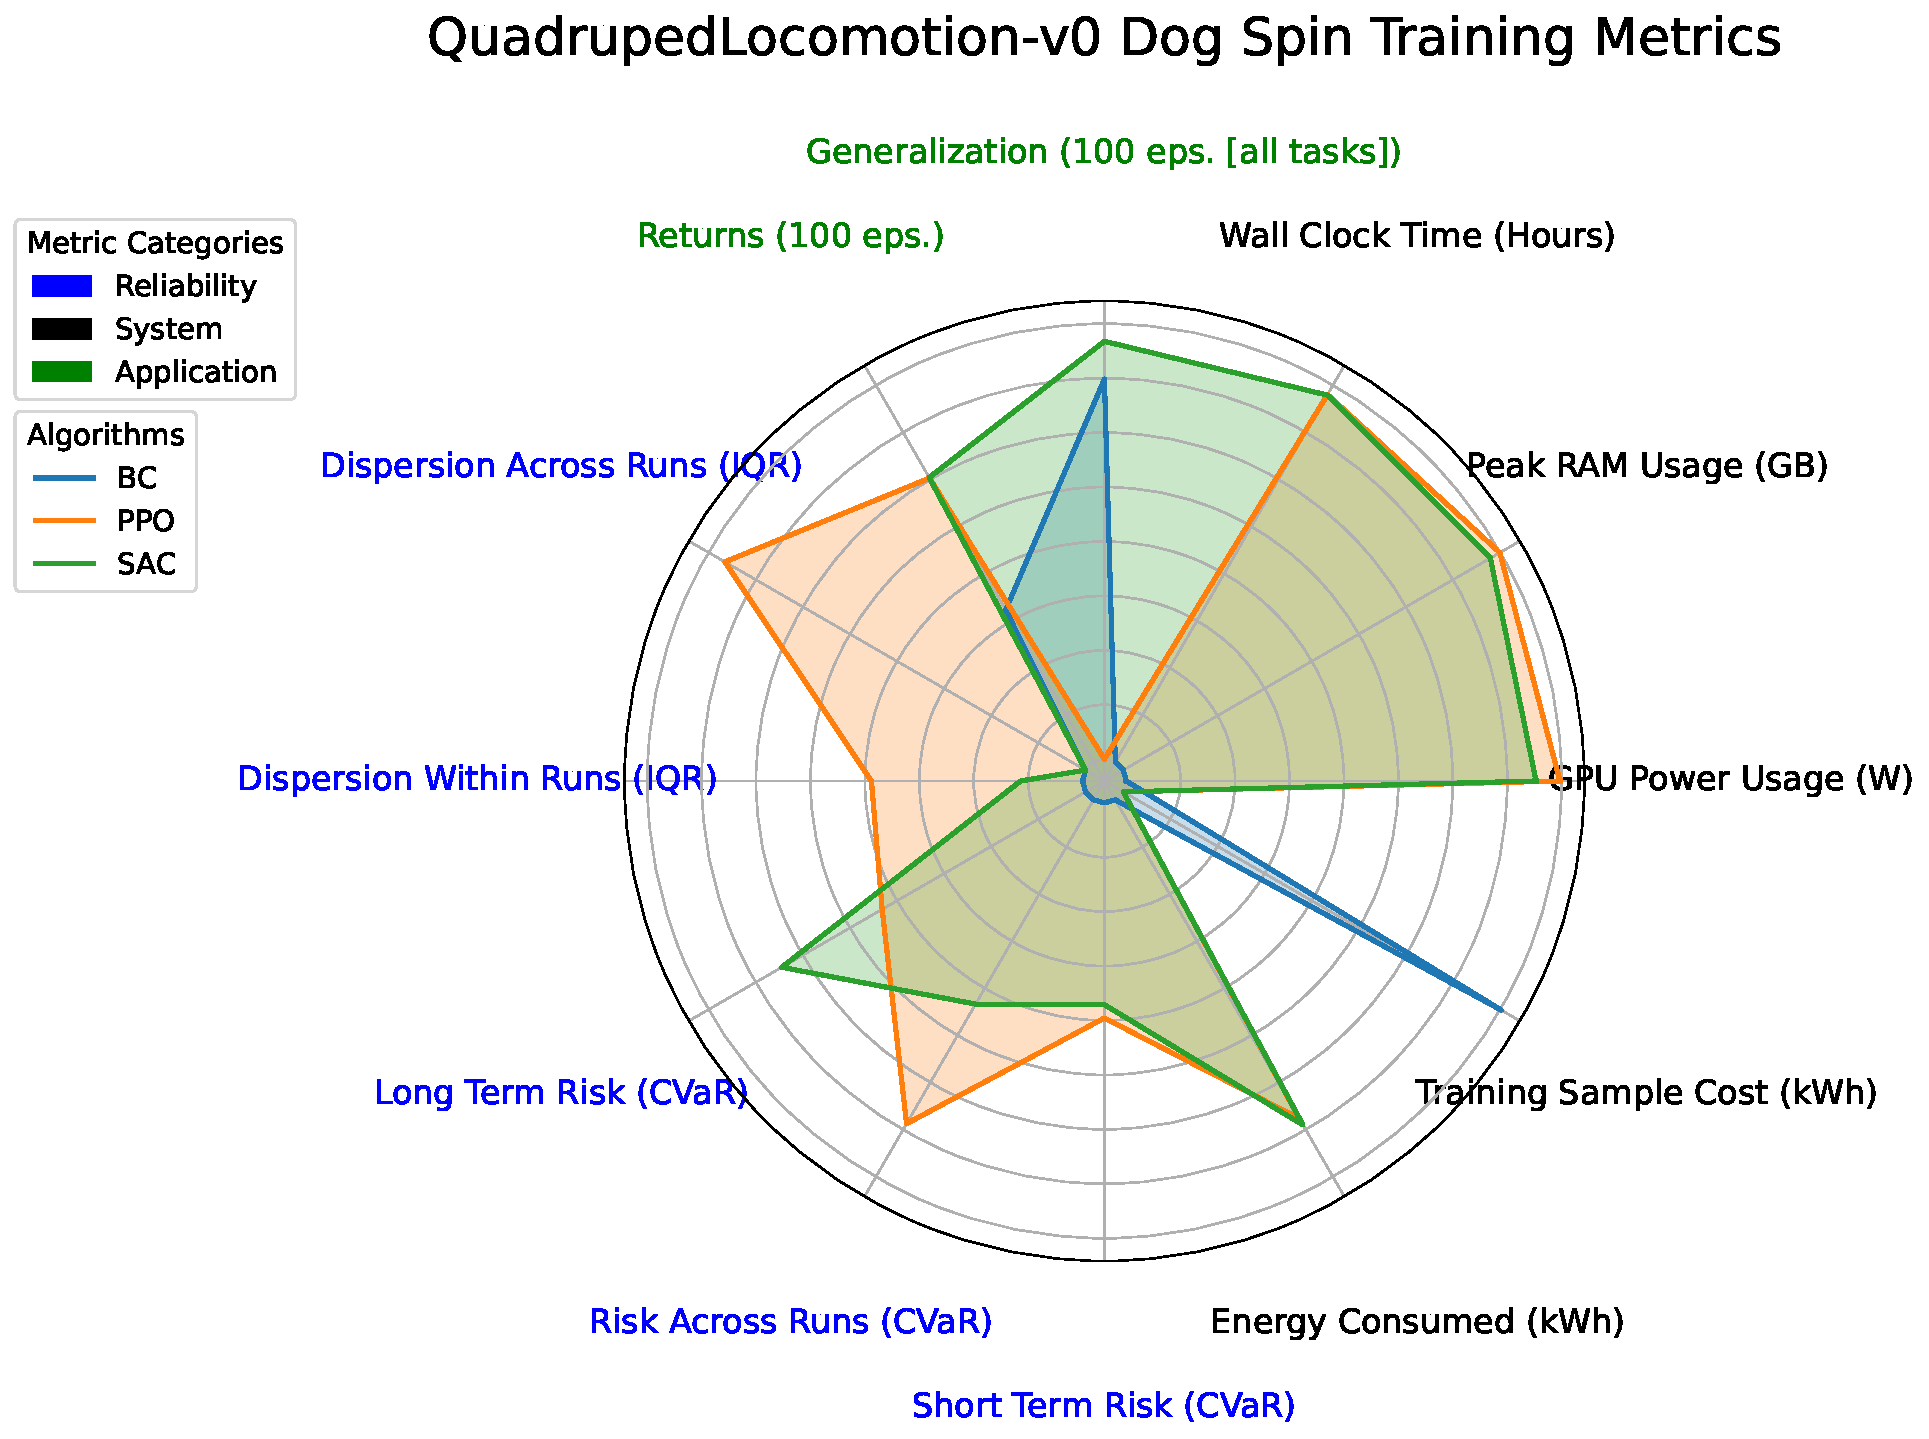
\includegraphics[width=\linewidth]{img/quadruped_locomotion/QuadrupedLocomotion-v0 Dog Spin Training Metrics.pdf}
%     \caption{Locomotion Spin Training Metrics}
%     \label{fig:image1}
%   \end{minipage}
%   \hfill % optional; adds horizontal spacing
%   \begin{minipage}[b]{0.4625\linewidth}
%     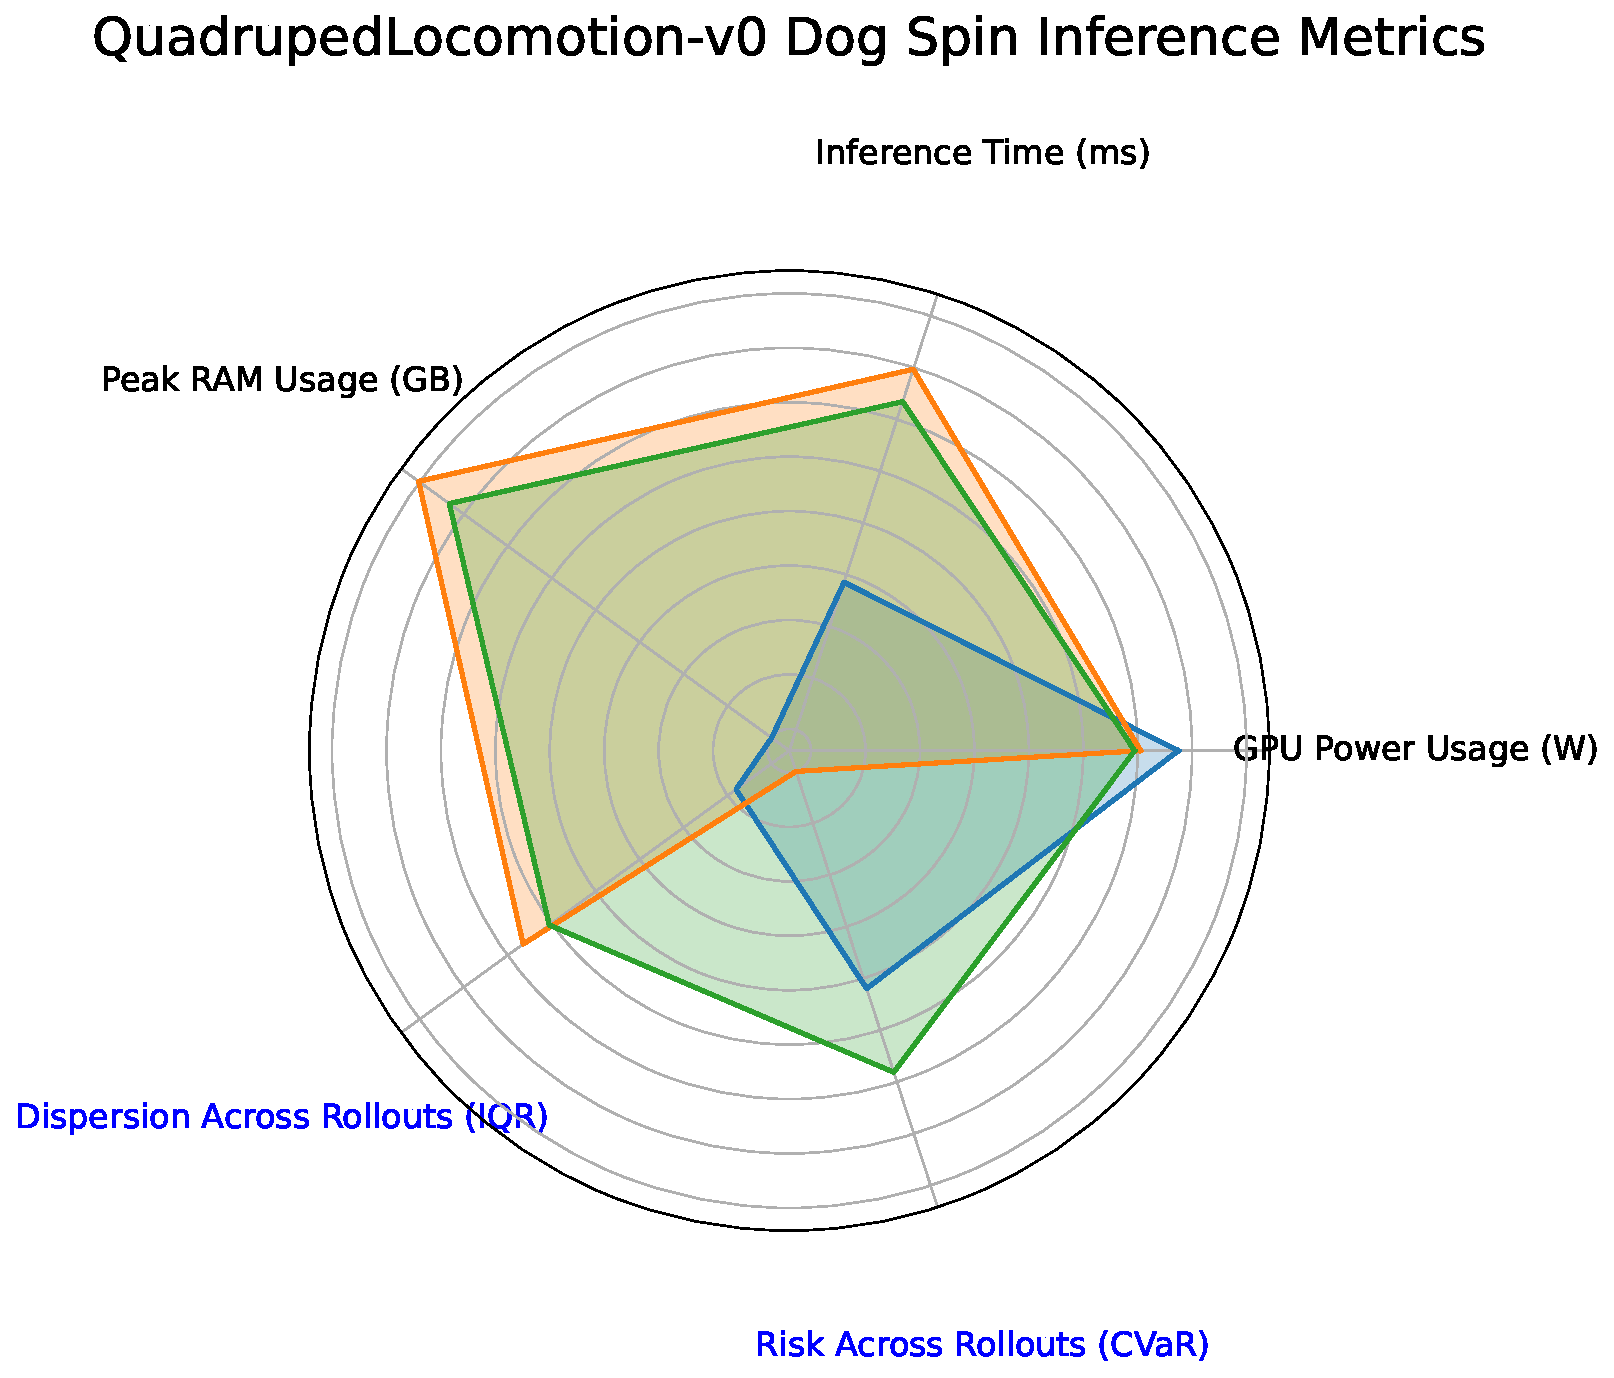
\includegraphics[width=\linewidth]{img/quadruped_locomotion/QuadrupedLocomotion-v0 Dog Spin Inference Metrics.pdf}
%     \caption{Locomotion Spin Inference Metrics}
%     \label{fig:image2}
%   \end{minipage}
% \end{figure}
% ---- Locomotion Spin
\begin{figure}[!htbp]
  \centering
  \begin{minipage}[b]{0.53\linewidth}
    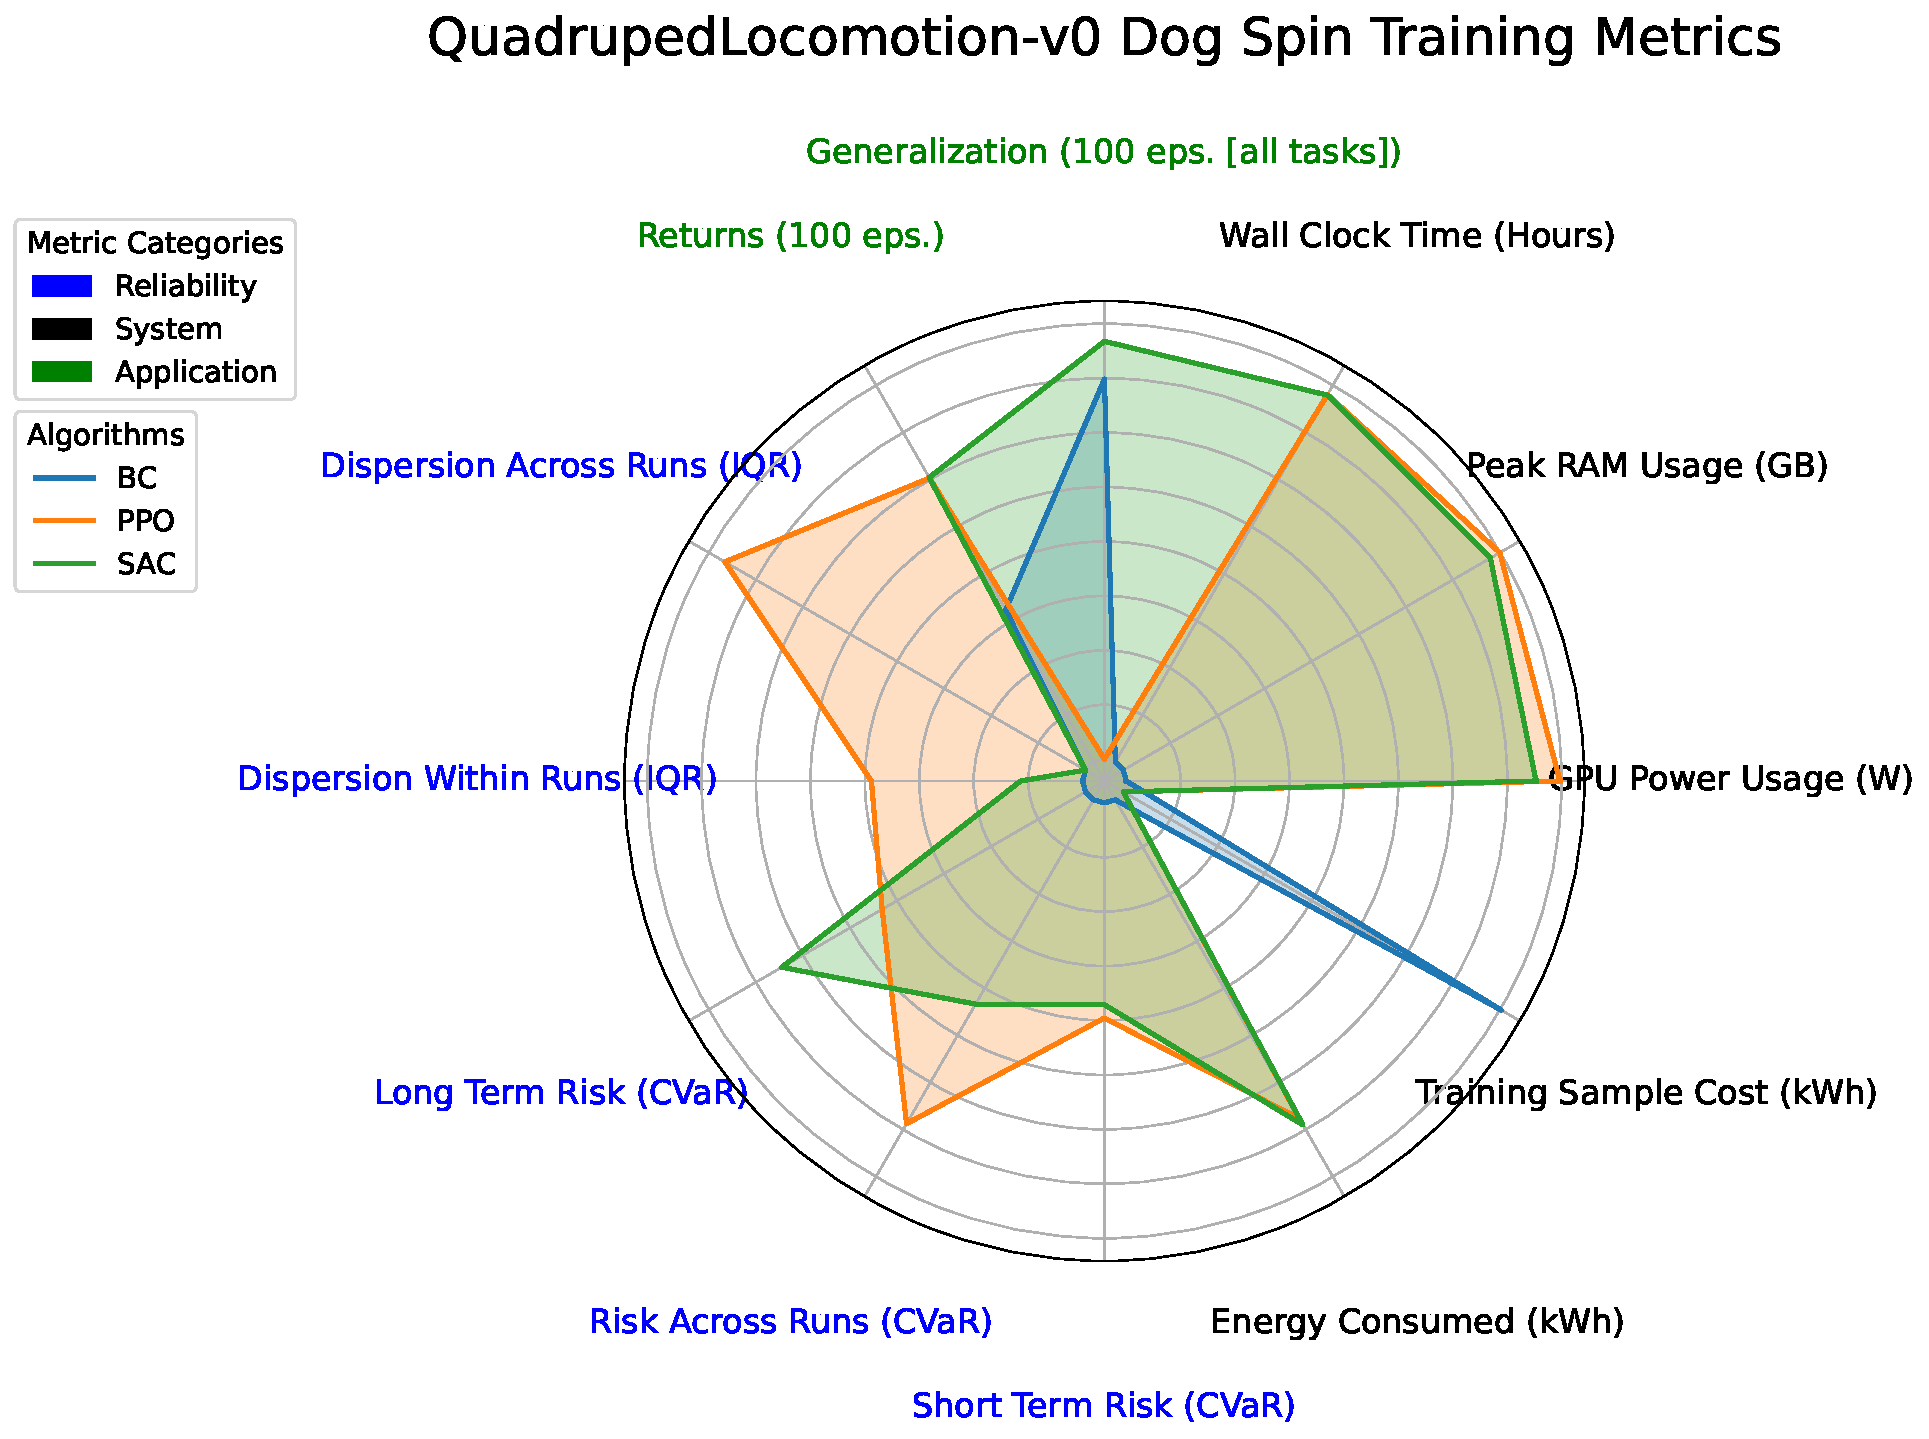
\includegraphics[width=\linewidth]{img/quadruped_locomotion/QuadrupedLocomotion-v0 Dog Spin Training Metrics.pdf}
  \end{minipage}
  \hfill % optional; adds horizontal spacing
  \begin{minipage}[b]{0.4625\linewidth}
    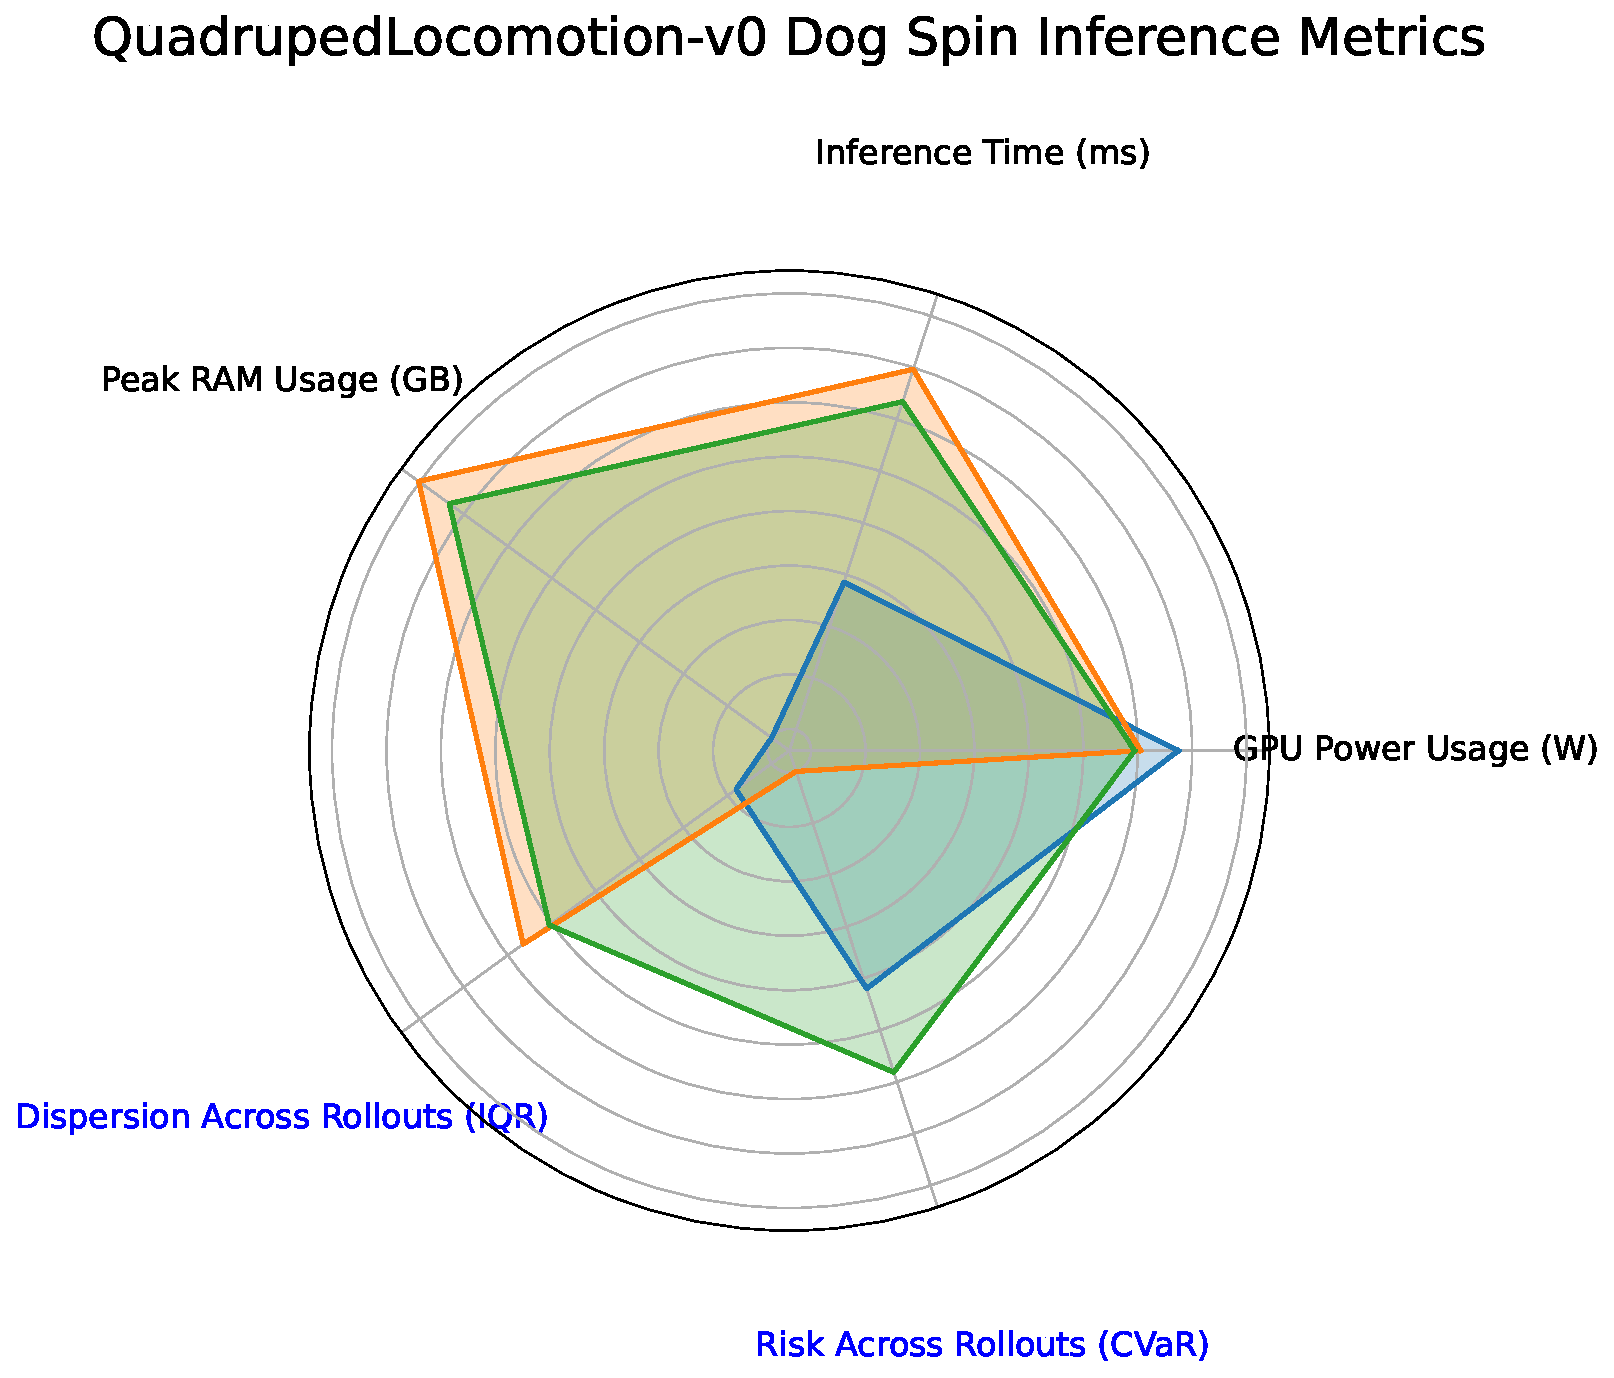
\includegraphics[width=\linewidth]{img/quadruped_locomotion/QuadrupedLocomotion-v0 Dog Spin Inference Metrics.pdf}
  \end{minipage}
  \caption{Graphical representation of metrics for the "dog spin" gait of QuadrupedLocomotion-v0}
  \label{fig:appendix_radar_quadruped_locomotion_dog_spin}
\end{figure}



% ---- Locomotion Trot
\begin{figure}[!htbp]
  \centering
  \begin{minipage}[b]{0.53\linewidth}
    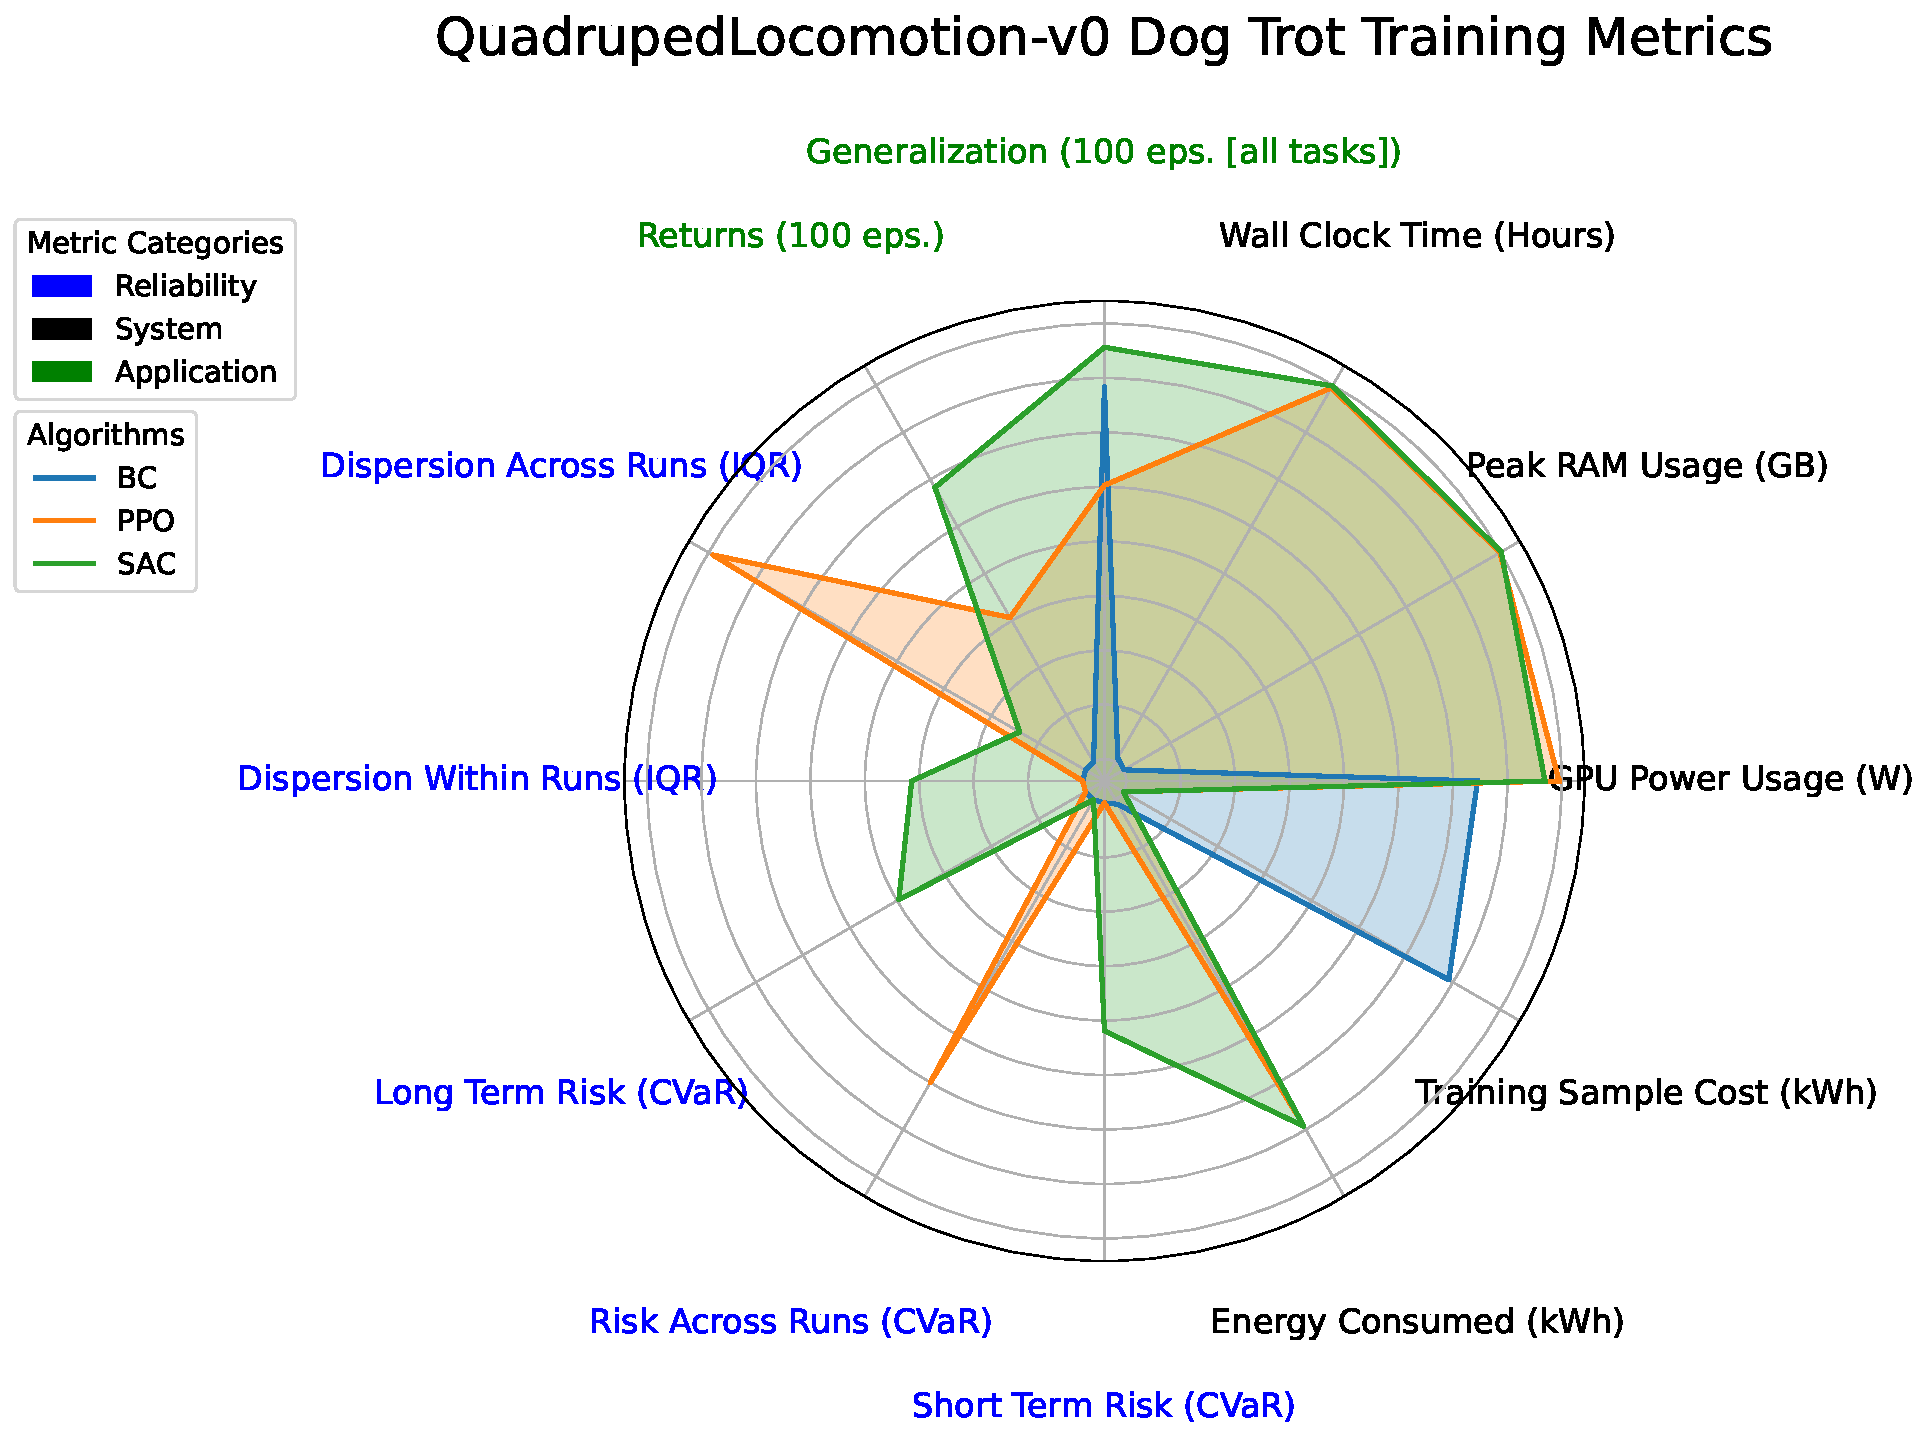
\includegraphics[width=\linewidth]{img/quadruped_locomotion/QuadrupedLocomotion-v0 Dog Trot Training Metrics.pdf}
  \end{minipage}
  \hfill % optional; adds horizontal spacing
  \begin{minipage}[b]{0.4625\linewidth}
    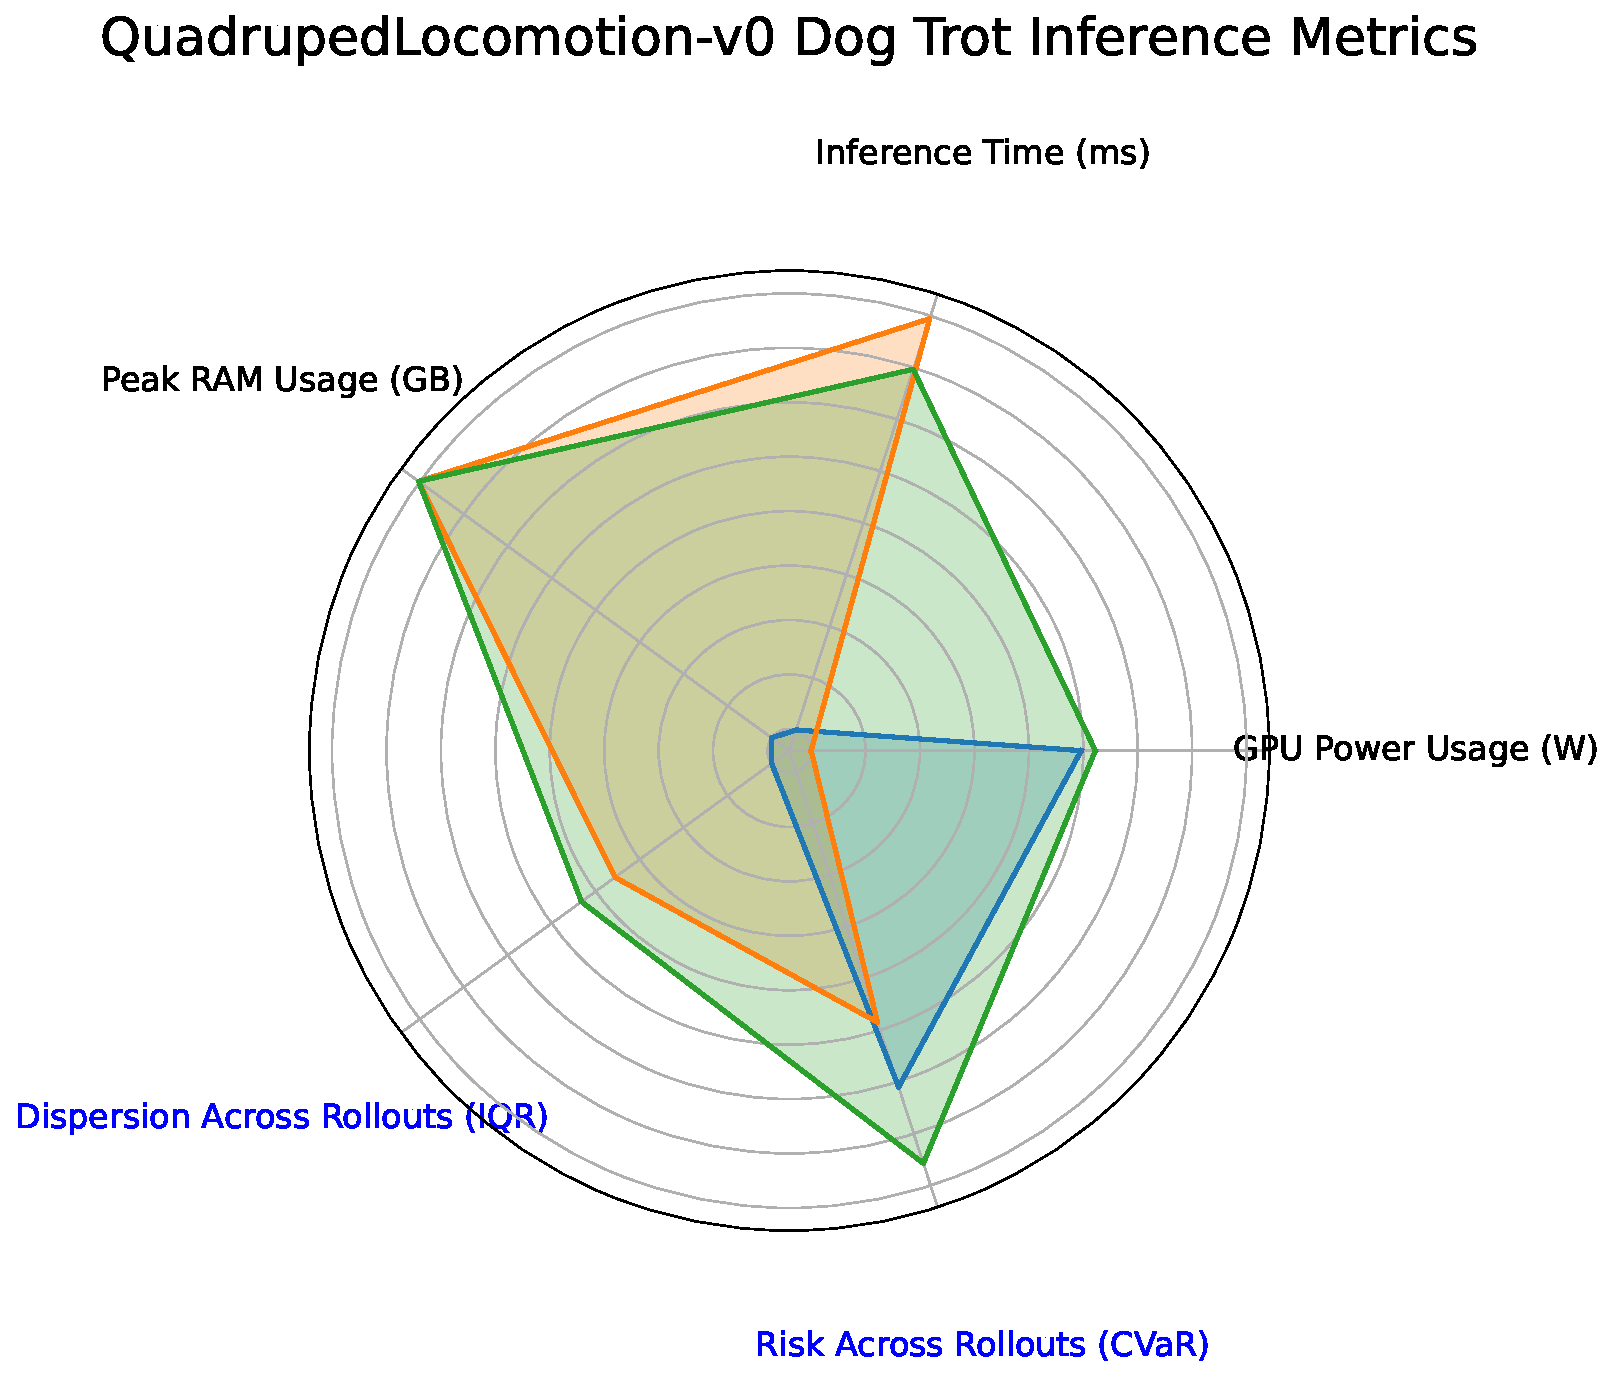
\includegraphics[width=\linewidth]{img/quadruped_locomotion/QuadrupedLocomotion-v0 Dog Trot Inference Metrics.pdf}
  \end{minipage}
  \caption{Graphical representation of metrics for the "dog trot" gait of QuadrupedLocomotion-v0}
  \label{fig:appendix_radar_quadruped_locomotion_dog_trot}
\end{figure}
% ---- Locomotion Pace
\begin{figure}[H]
  \centering
  \begin{minipage}[b]{0.53\linewidth}
    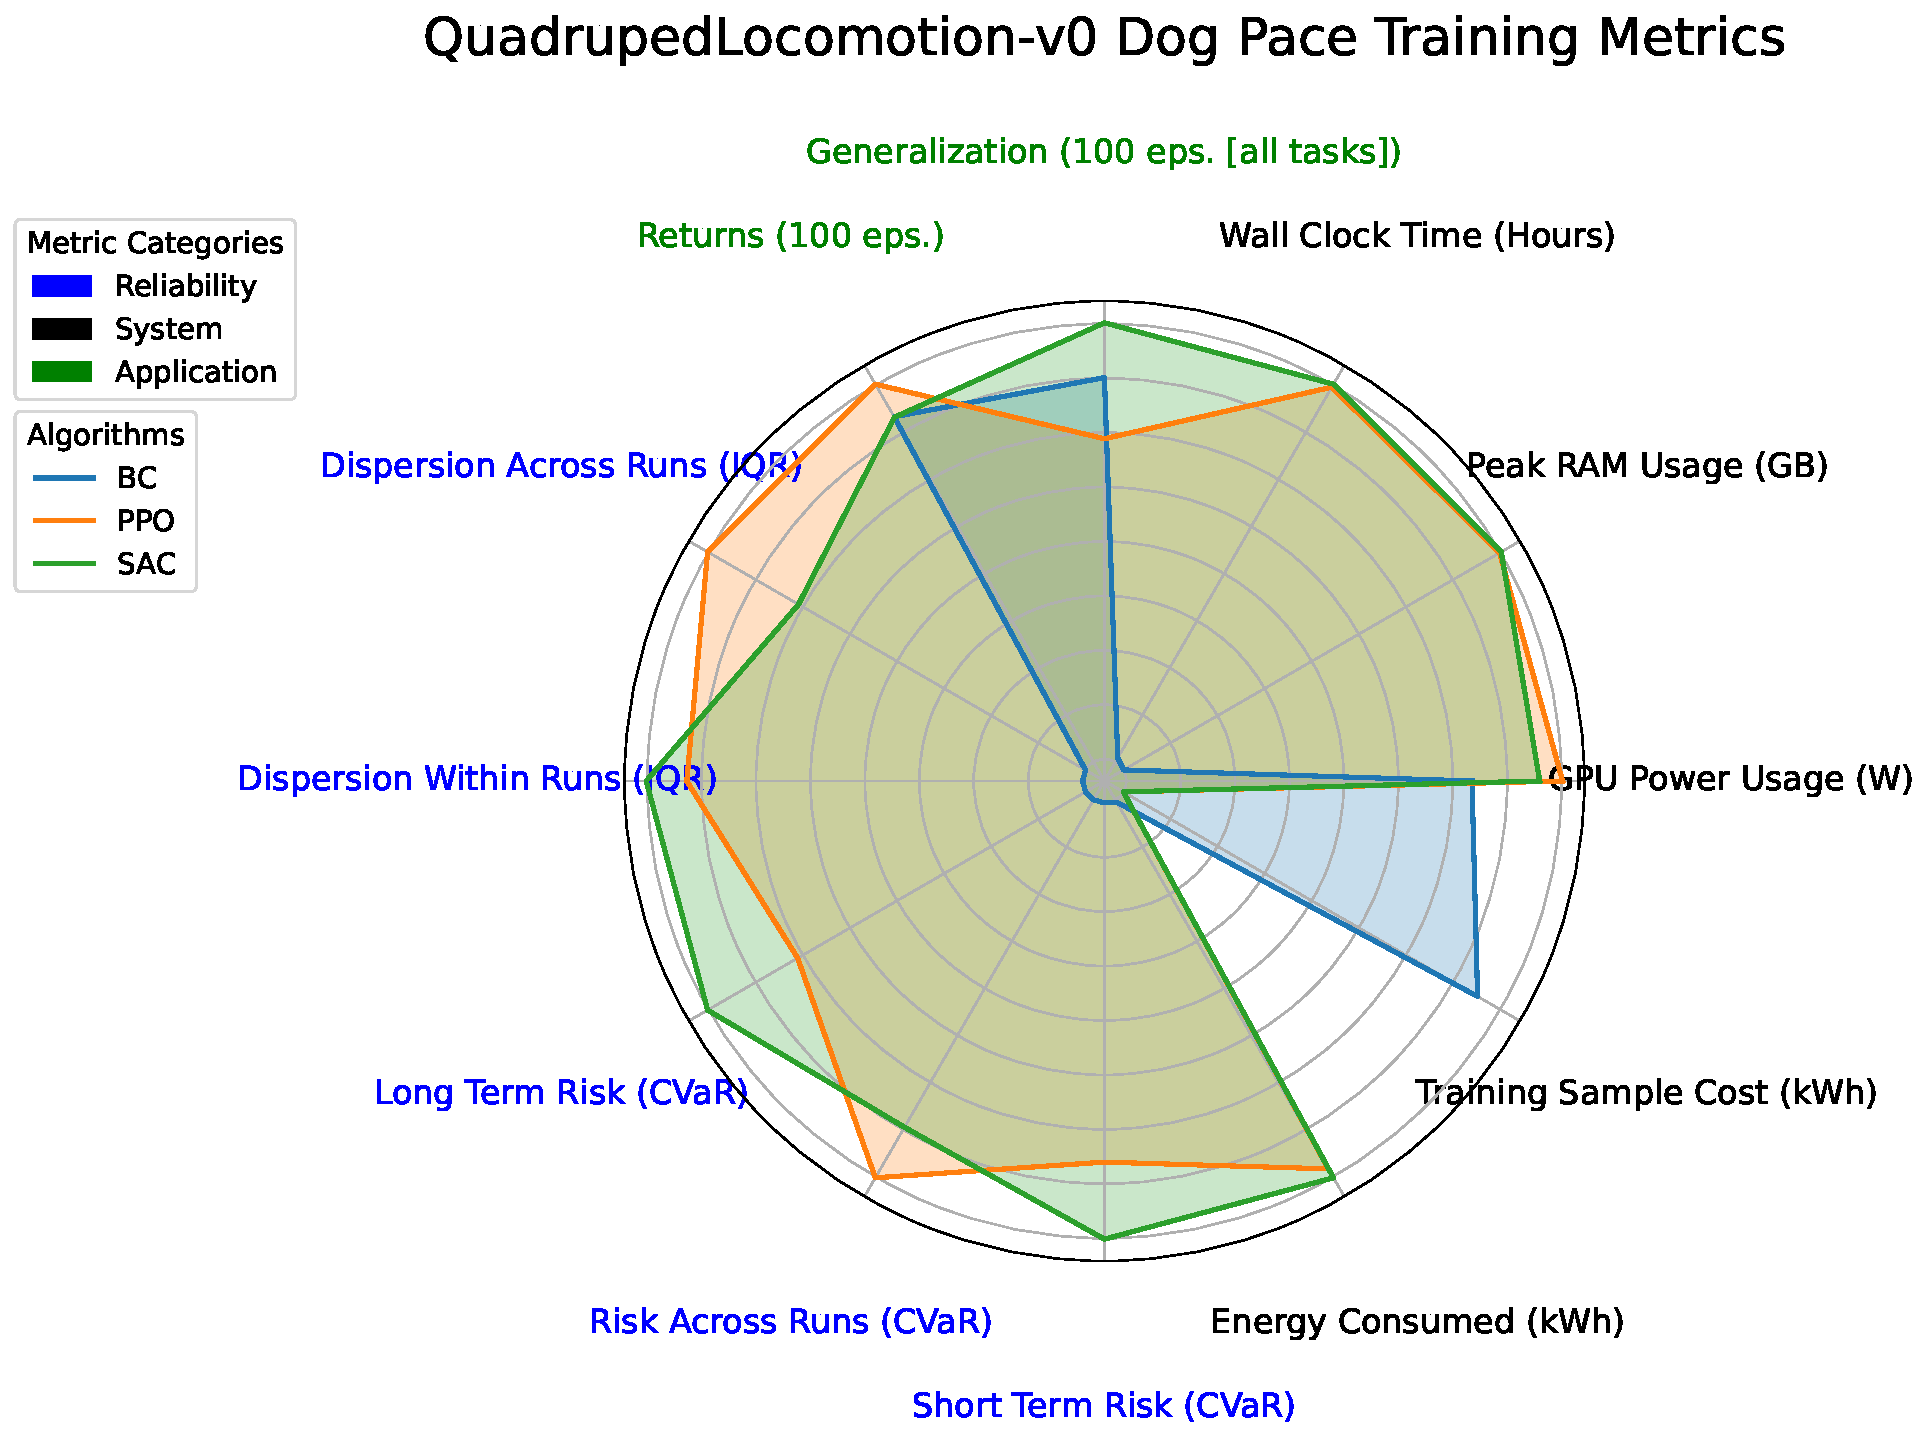
\includegraphics[width=\linewidth]{img/quadruped_locomotion/QuadrupedLocomotion-v0 Dog Pace Training Metrics.pdf}
  \end{minipage}
  \hfill % optional; adds horizontal spacing
  \begin{minipage}[b]{0.4625\linewidth}
    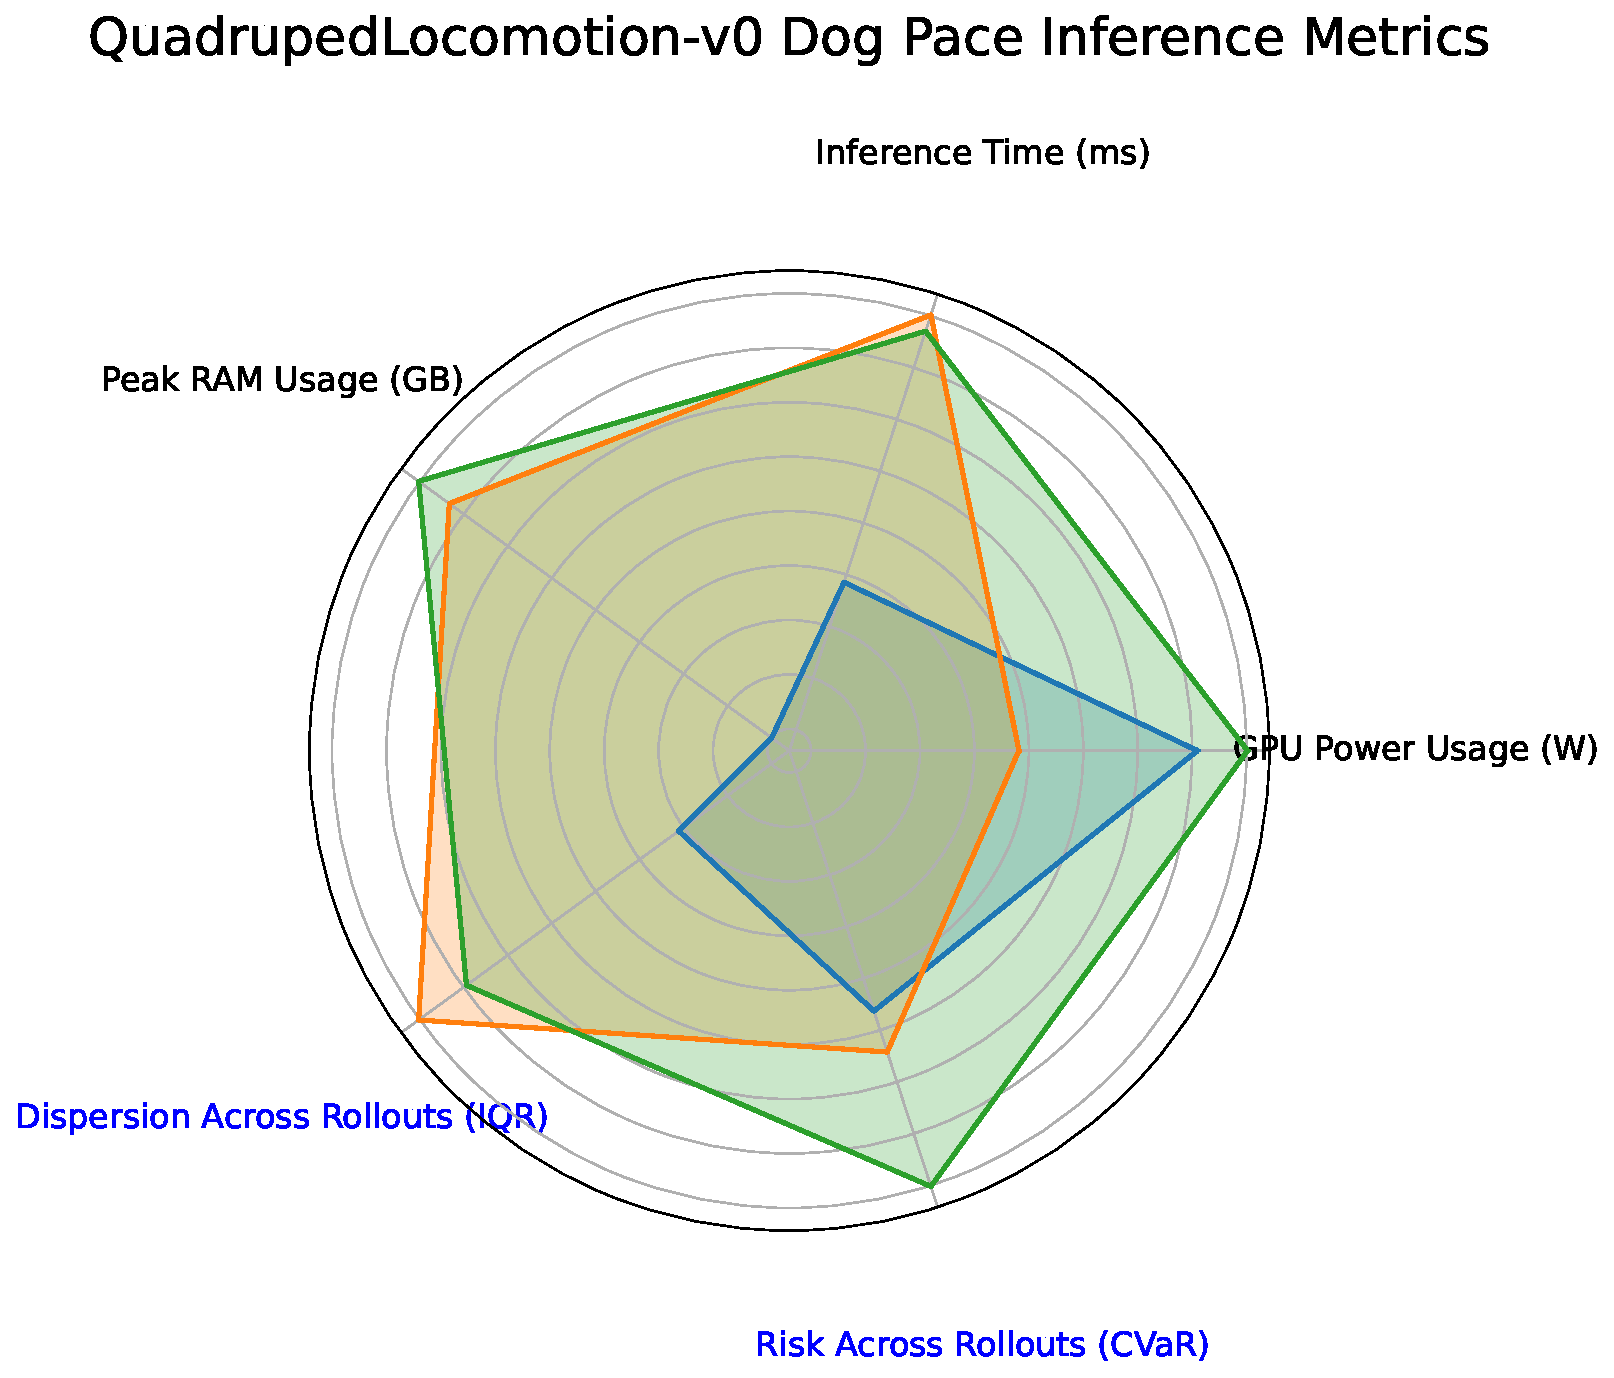
\includegraphics[width=\linewidth]{img/quadruped_locomotion/QuadrupedLocomotion-v0 Dog Pace Inference Metrics.pdf}
  \end{minipage}
  \caption{Graphical representation of metrics for the "dog pace" gait of QuadrupedLocomotion-v0}
  \label{fig:appendix_radar_quadruped_locomotion_dog_pace}
\end{figure}

\newpage

% ---- Circuit Training Toy
\begin{figure}[!htbp]
  \centering
  \begin{minipage}[b]{0.53\linewidth}
    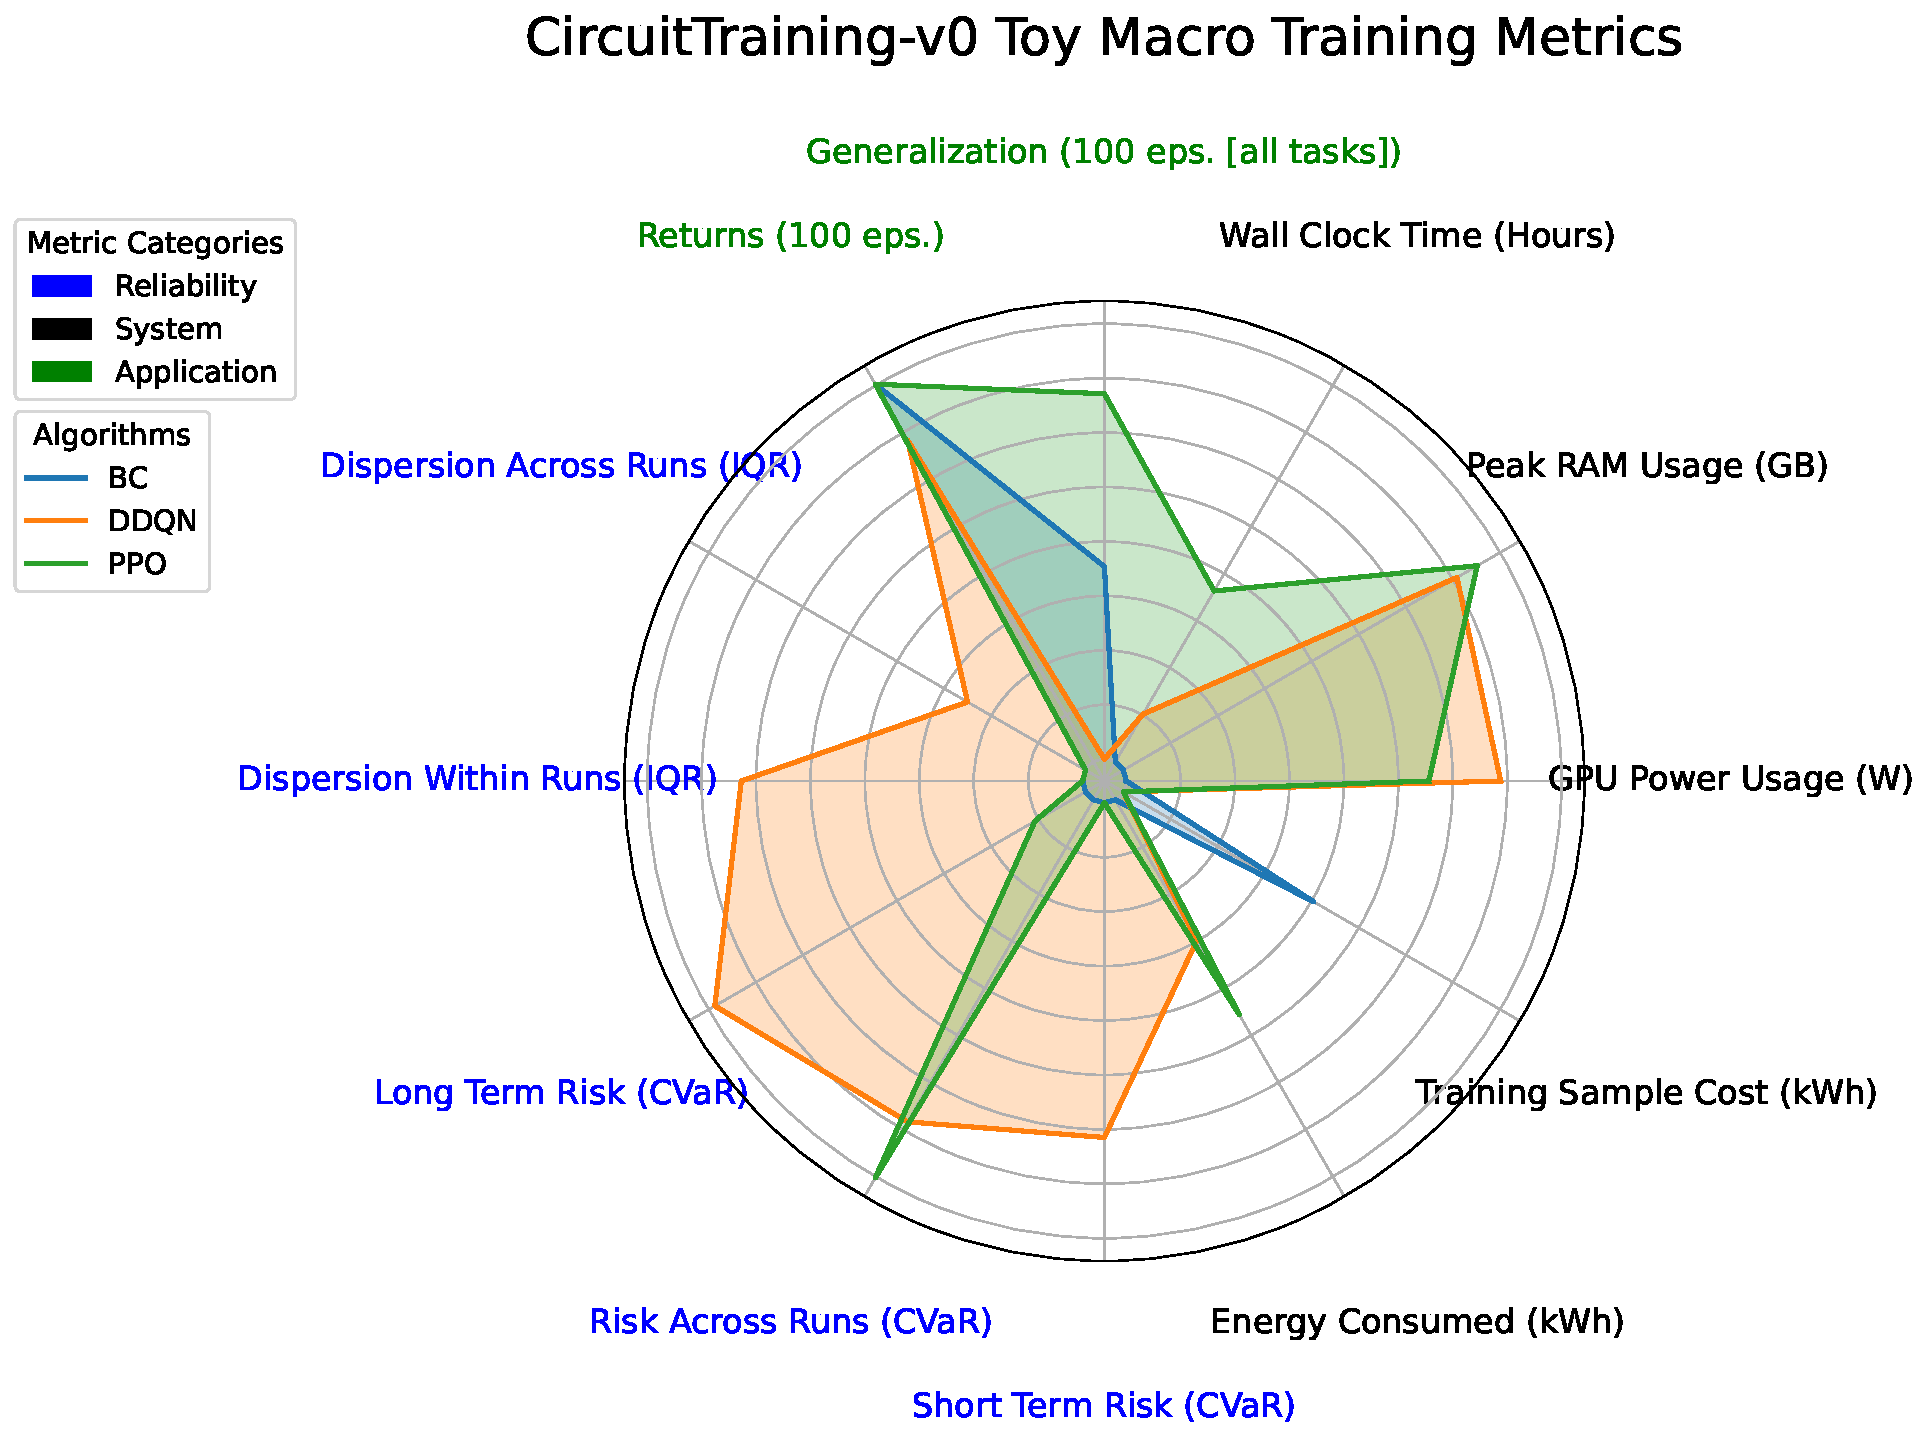
\includegraphics[width=\linewidth]{img/circuit_training/CircuitTraining-v0 Toy Macro Training Metrics.pdf}
  \end{minipage}
  \hfill % optional; adds horizontal spacing
  \begin{minipage}[b]{0.44\linewidth}
    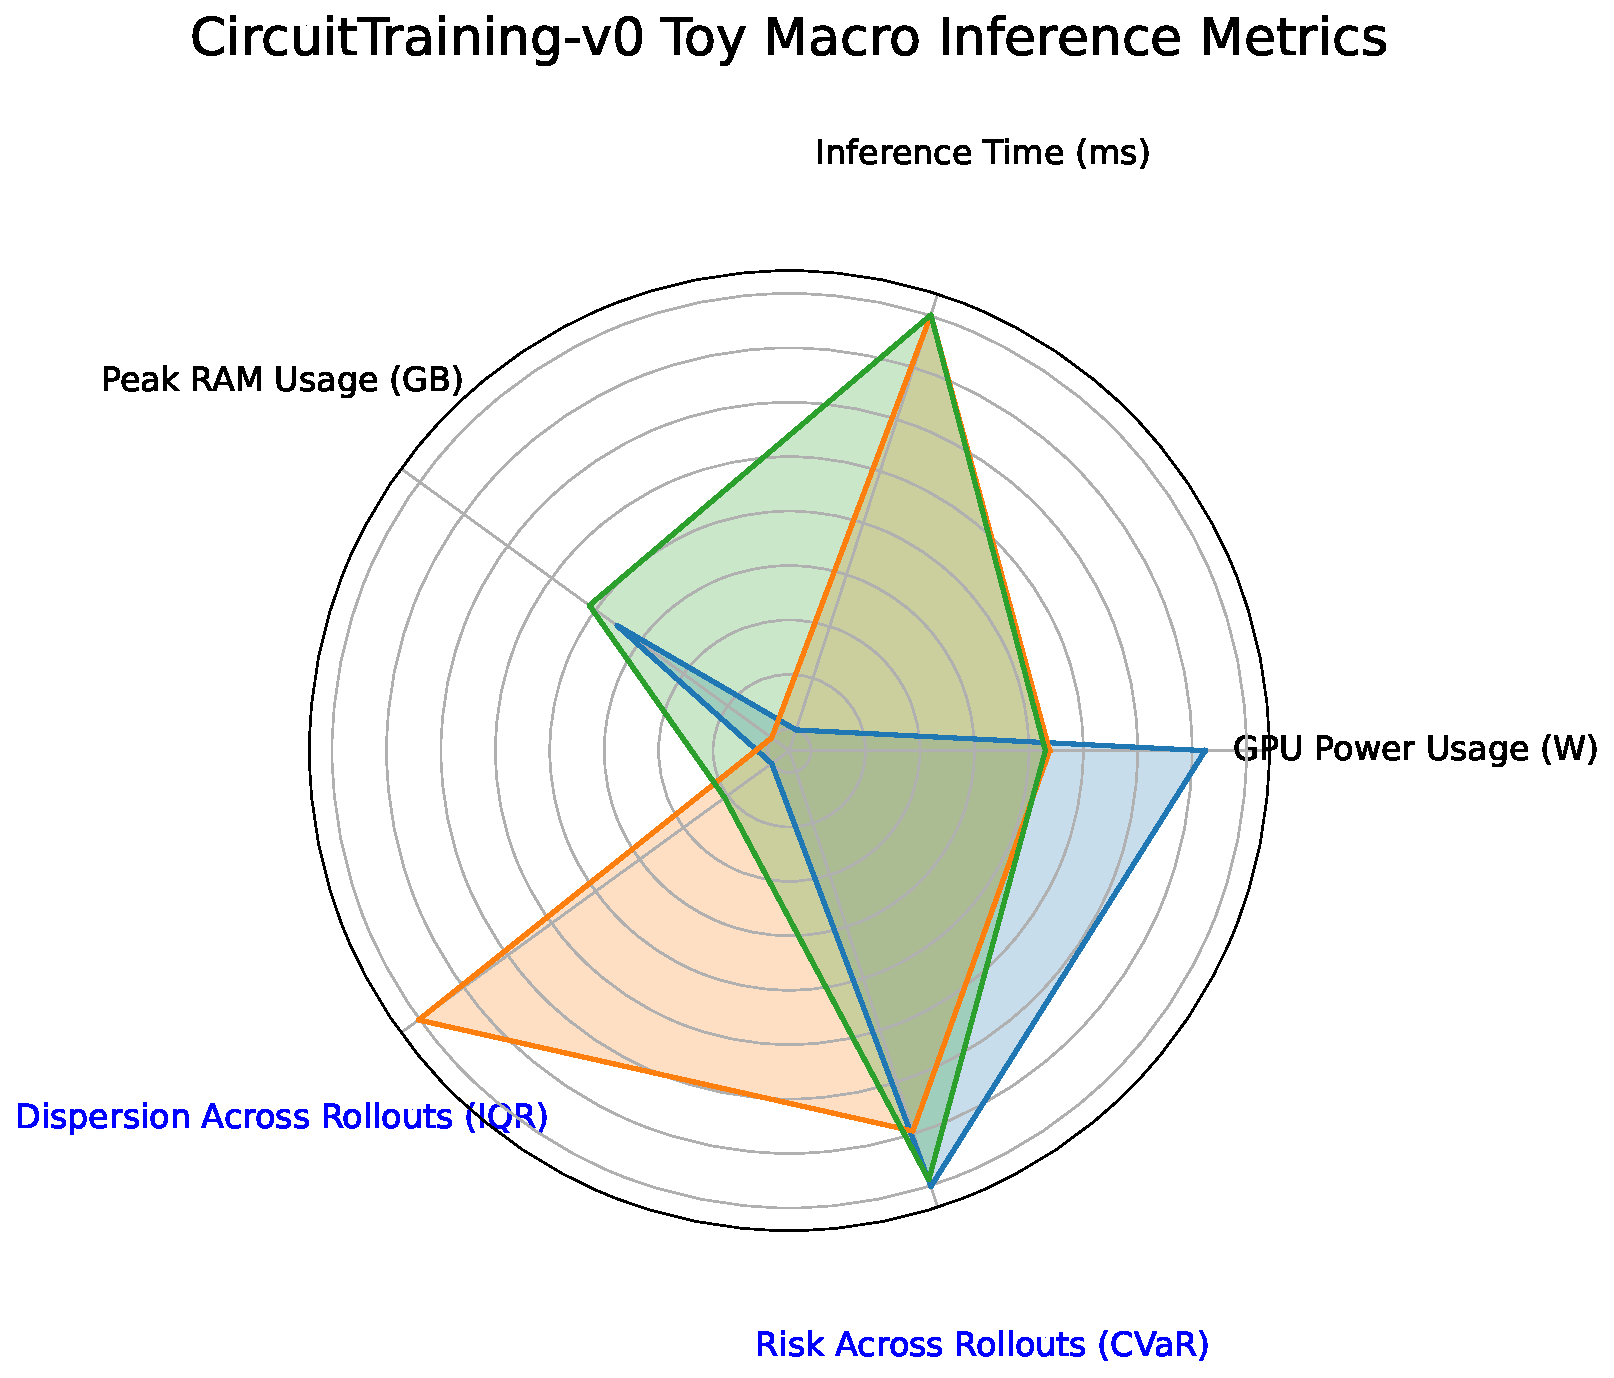
\includegraphics[width=\linewidth]{img/circuit_training/CircuitTraining-v0 Toy Macro Inference Metrics.pdf}
  \end{minipage}
  \caption{Graphical representation of metrics for the "Toy Macro" netlist task of CircuitTraining-v0}
  \label{fig:appendix_circuit_training_toy_macro}
\end{figure}


% ---- Circuit Training Ariane
\begin{figure}[!htbp]
  \centering
  \begin{minipage}[b]{0.53\linewidth}
    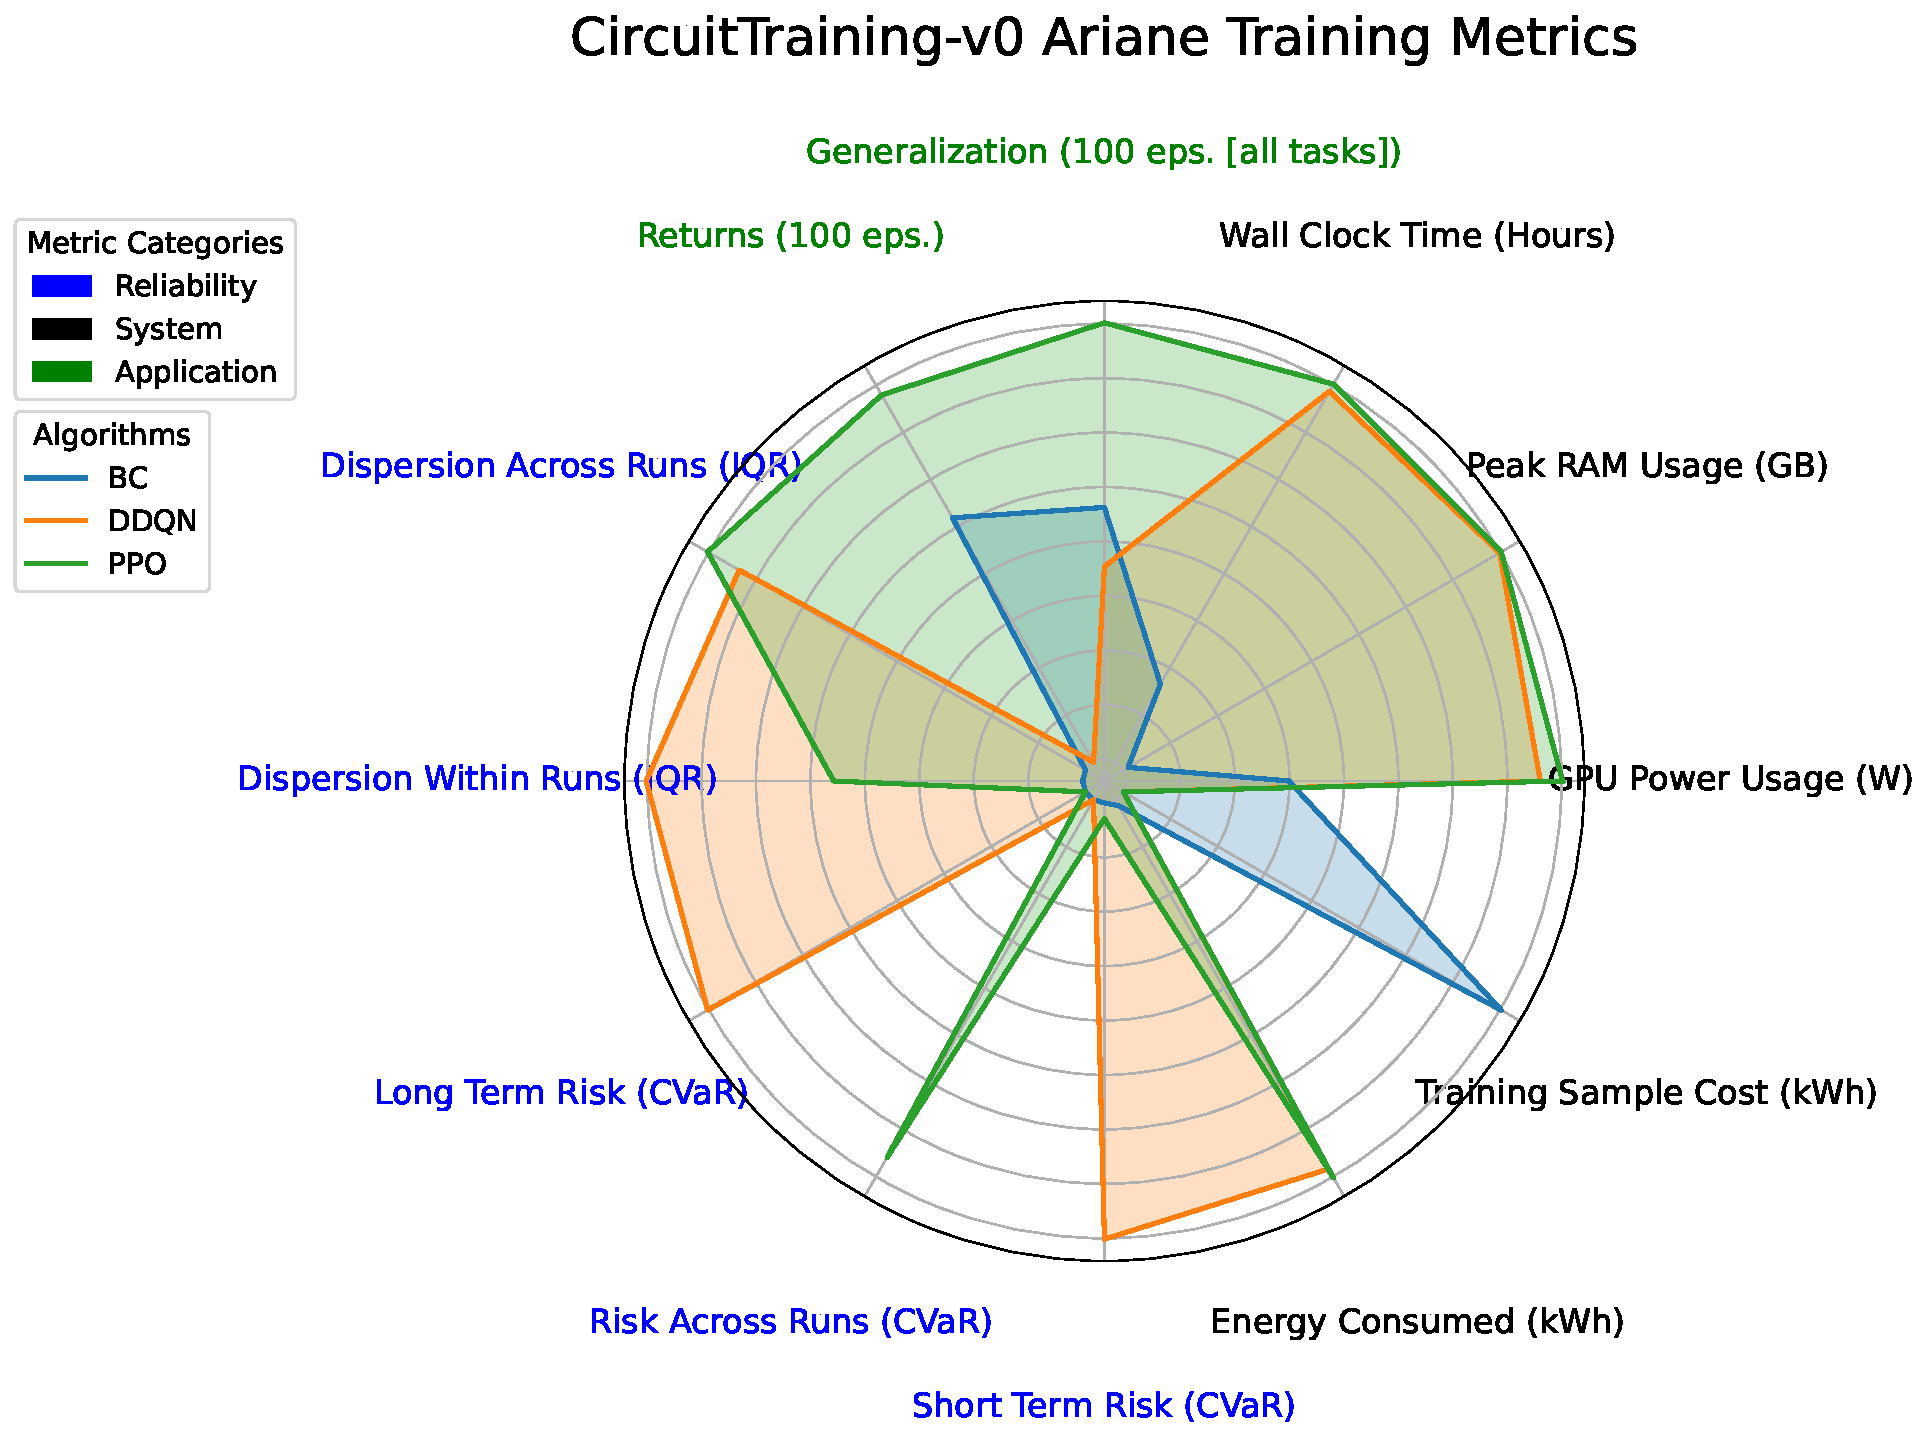
\includegraphics[width=\linewidth]{img/circuit_training/CircuitTraining-v0 Ariane Training Metrics.pdf}
  \end{minipage}
  \hfill % optional; adds horizontal spacing
  \begin{minipage}[b]{0.44\linewidth}
    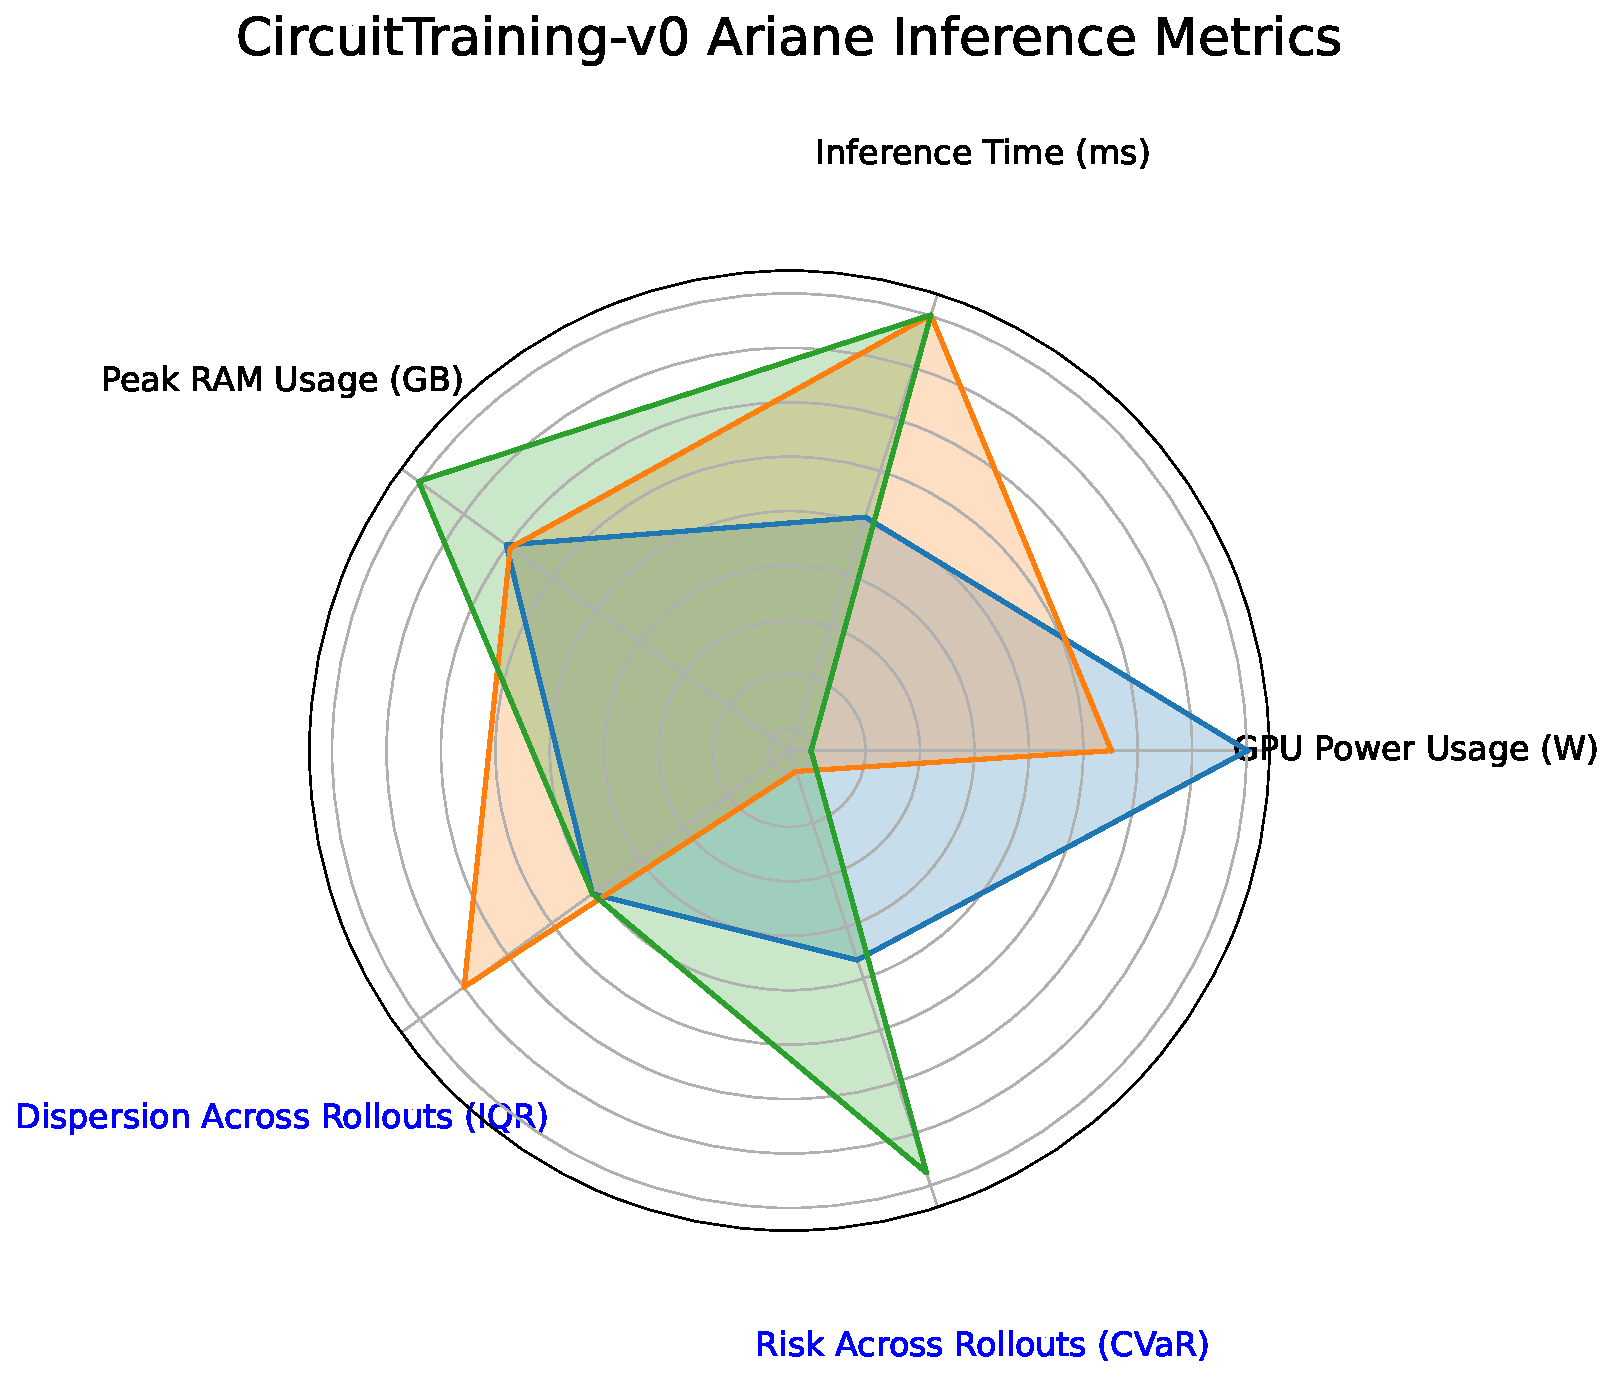
\includegraphics[width=\linewidth]{img/circuit_training/CircuitTraining-v0 Ariane Inference Metrics.pdf}
  \end{minipage}
  \caption{Graphical representation of metrics for the "Ariane" netlist task of CircuitTraining-v0}
  \label{fig:appendix_circuit_training_ariane}
\end{figure}
\newpage


% ---- WebNav 1 Website
\begin{figure}[!htbp]
  \centering
  \begin{minipage}[b]{0.53\linewidth}
    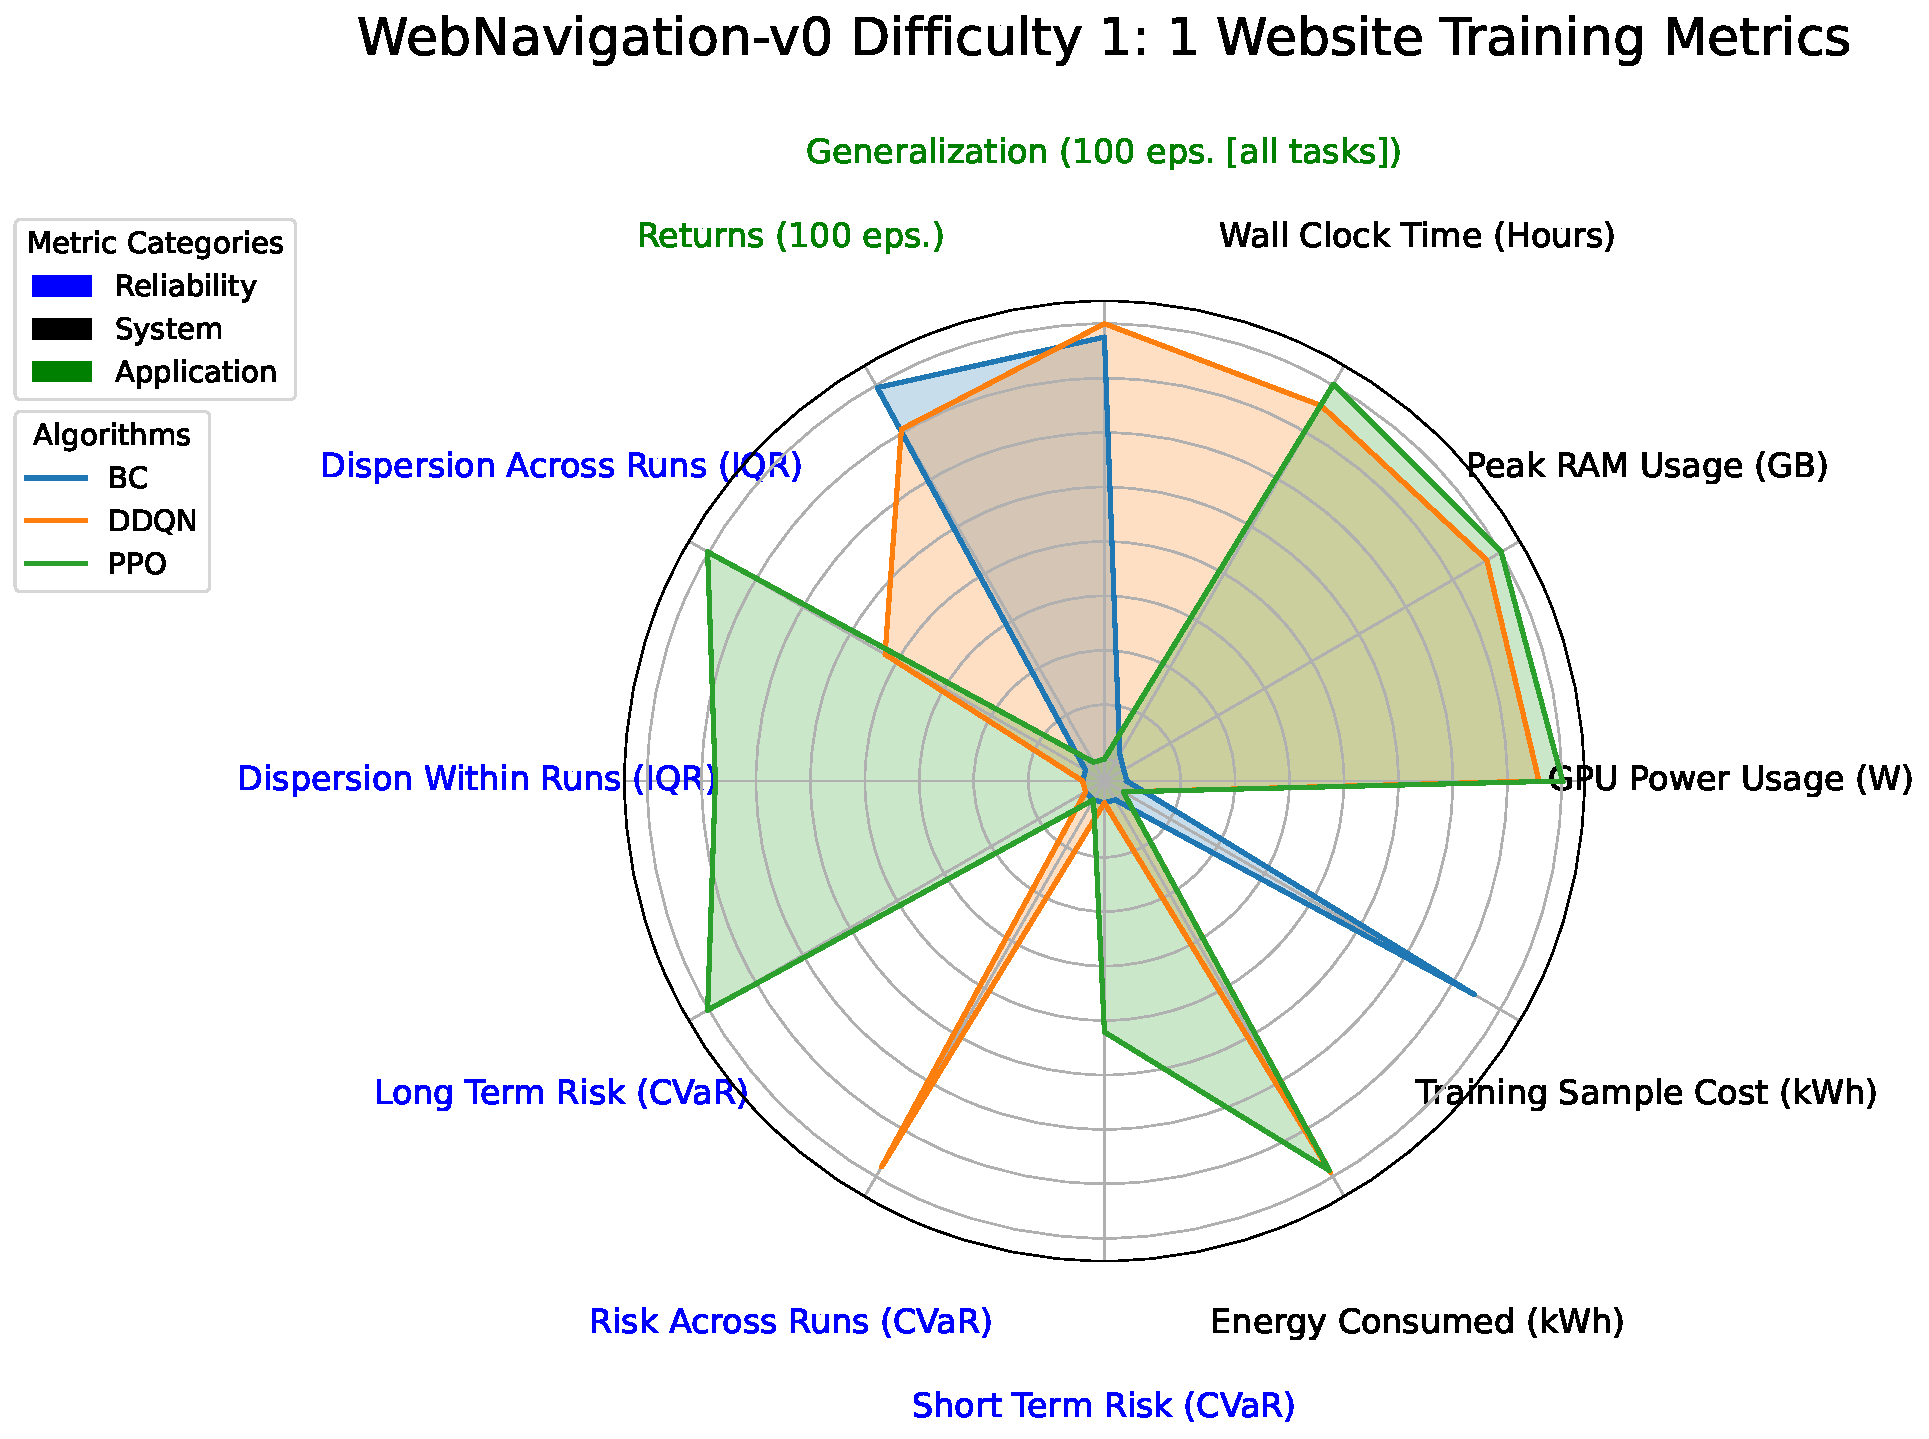
\includegraphics[width=\linewidth]{img/web_nav/WebNavigation-v0 Difficulty 1_ 1 Website Training Metrics.pdf}
  \end{minipage}
  \hfill % optional; adds horizontal spacing
  \begin{minipage}[b]{0.4625\linewidth}
    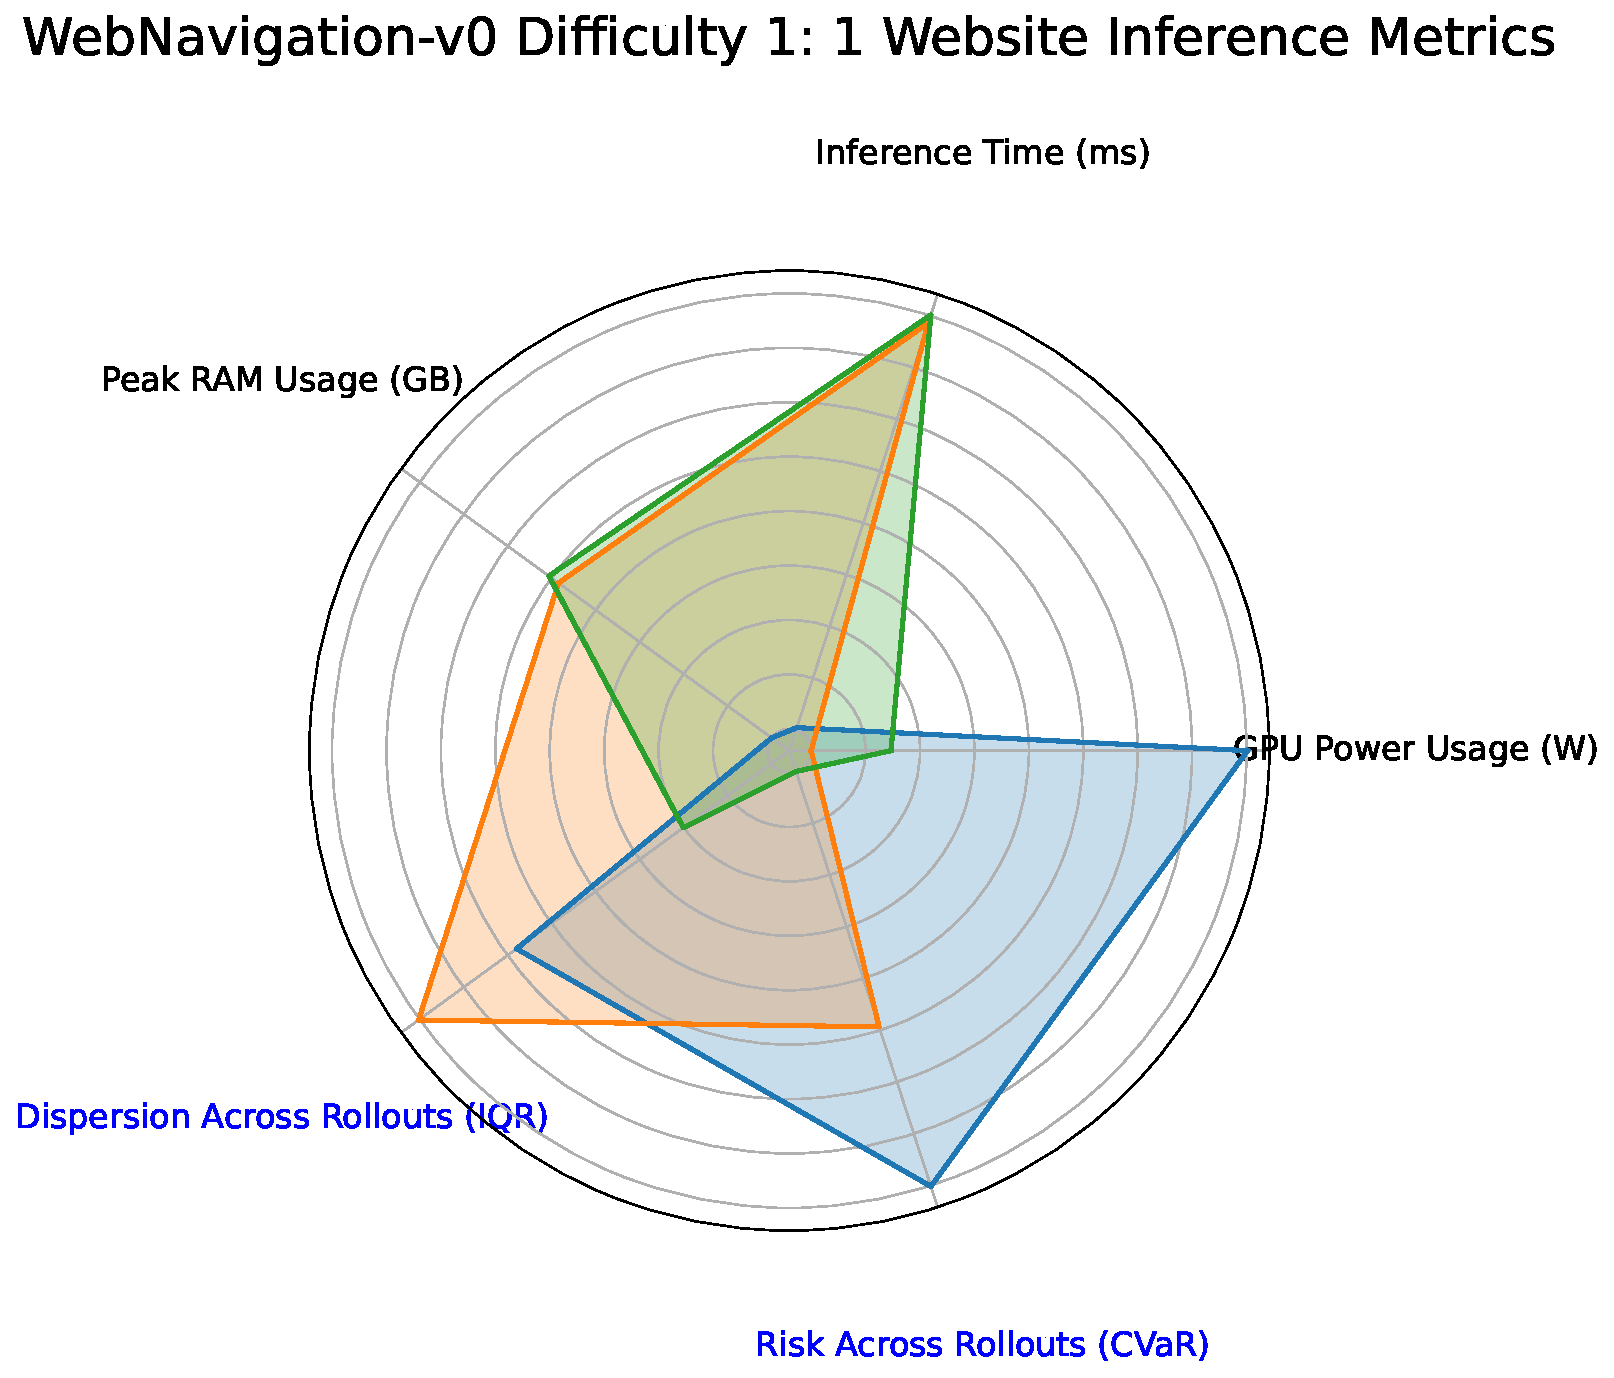
\includegraphics[width=\linewidth]{img/web_nav/WebNavigation-v0 Difficulty 1_ 1 Website Inference Metrics.pdf}
  \end{minipage}
  \caption{Graphical representation of metrics for the "difficulty 1, 1 website" task of WebNavigation-v0}
  \label{fig:appendix_radar_web_nav_difficulty1_1website}
\end{figure}


% ---- WebNav 5 Websites
\begin{figure}[!htbp]
  \centering
  \begin{minipage}[b]{0.53\linewidth}
    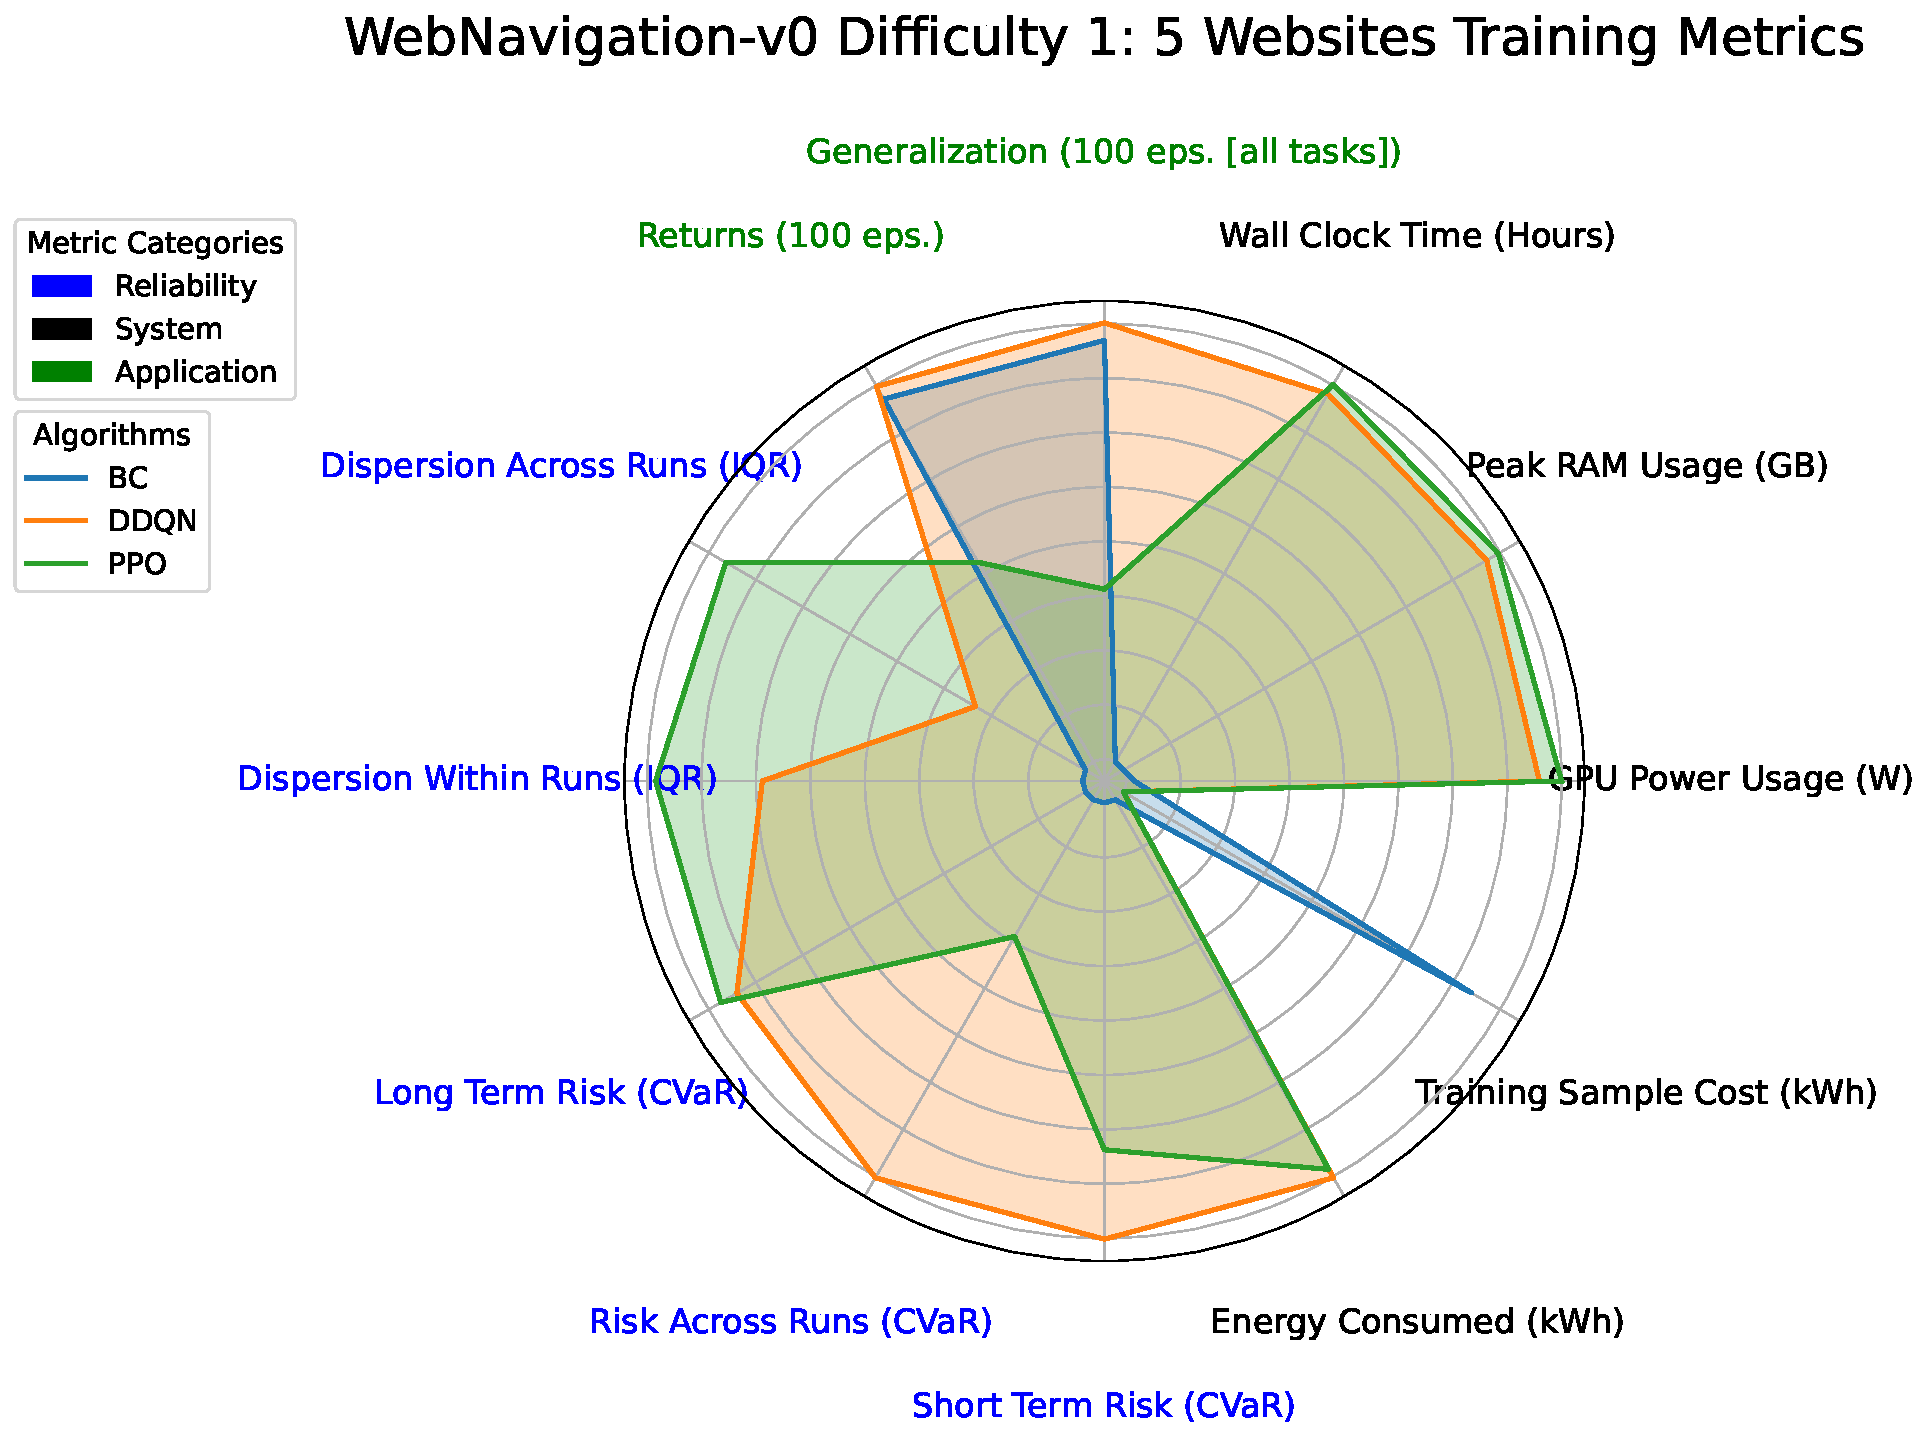
\includegraphics[width=\linewidth]{img/web_nav/WebNavigation-v0 Difficulty 1_ 5 Websites Training Metrics.pdf}
  \end{minipage}
  \hfill % optional; adds horizontal spacing
  \begin{minipage}[b]{0.4625\linewidth}
    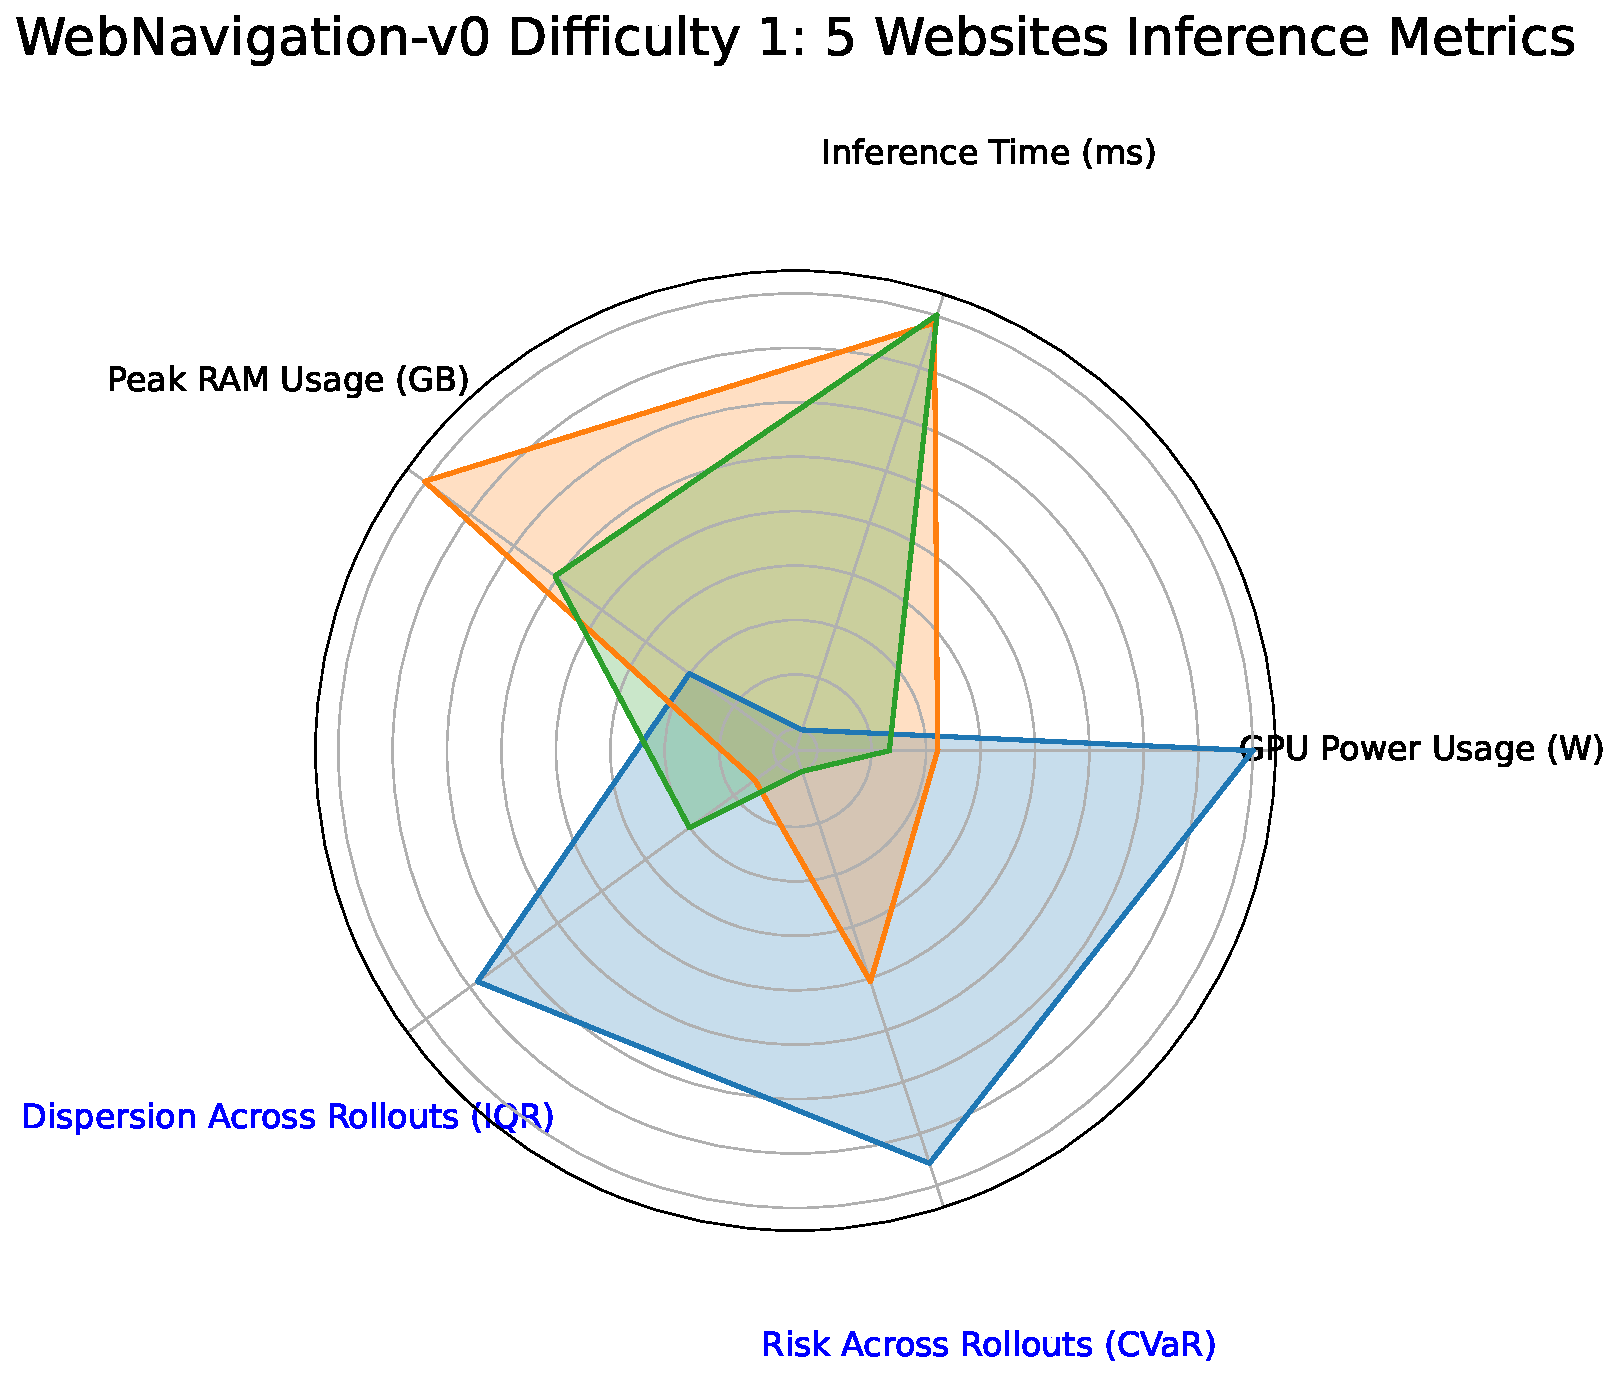
\includegraphics[width=\linewidth]{img/web_nav/WebNavigation-v0 Difficulty 1_ 5 Websites Inference Metrics.pdf}
  \end{minipage}
  \caption{Graphical representation of metrics for the "difficulty 1, 5 websites" task of WebNavigation-v0}
  \label{fig:appendix_radar_web_nav_difficulty1_5websites}
\end{figure}


% ---- WebNav 10 Websites
\begin{figure}[!htbp]
  \centering
  \begin{minipage}[b]{0.53\linewidth}
    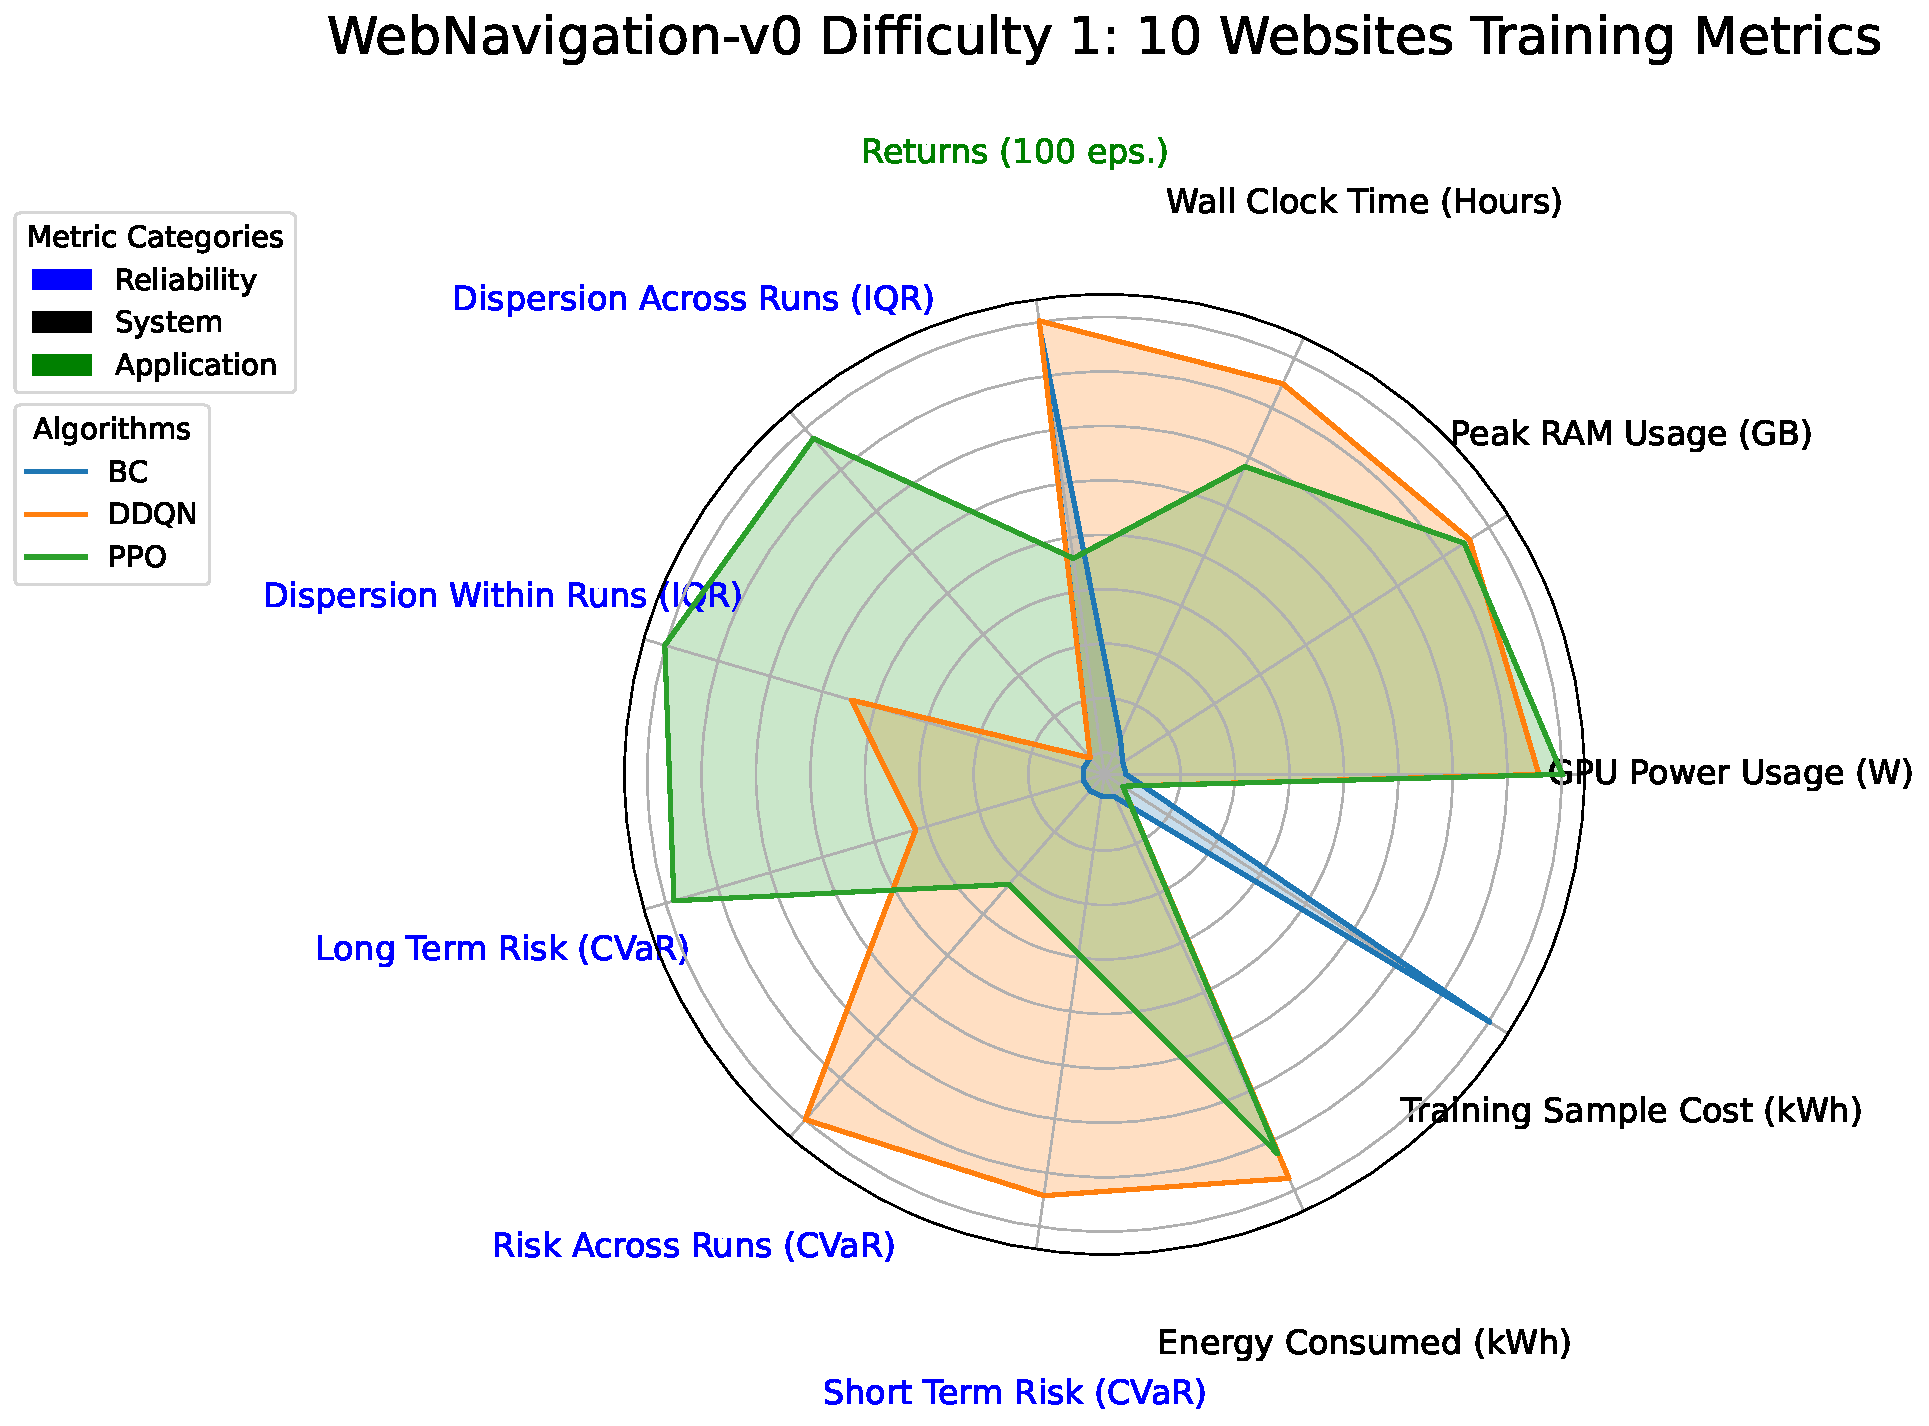
\includegraphics[width=\linewidth]{img/web_nav/WebNavigation-v0 Difficulty 1_ 10 Websites Training Metrics.pdf}
  \end{minipage}
  \hfill % optional; adds horizontal spacing
  \begin{minipage}[b]{0.4625\linewidth}
    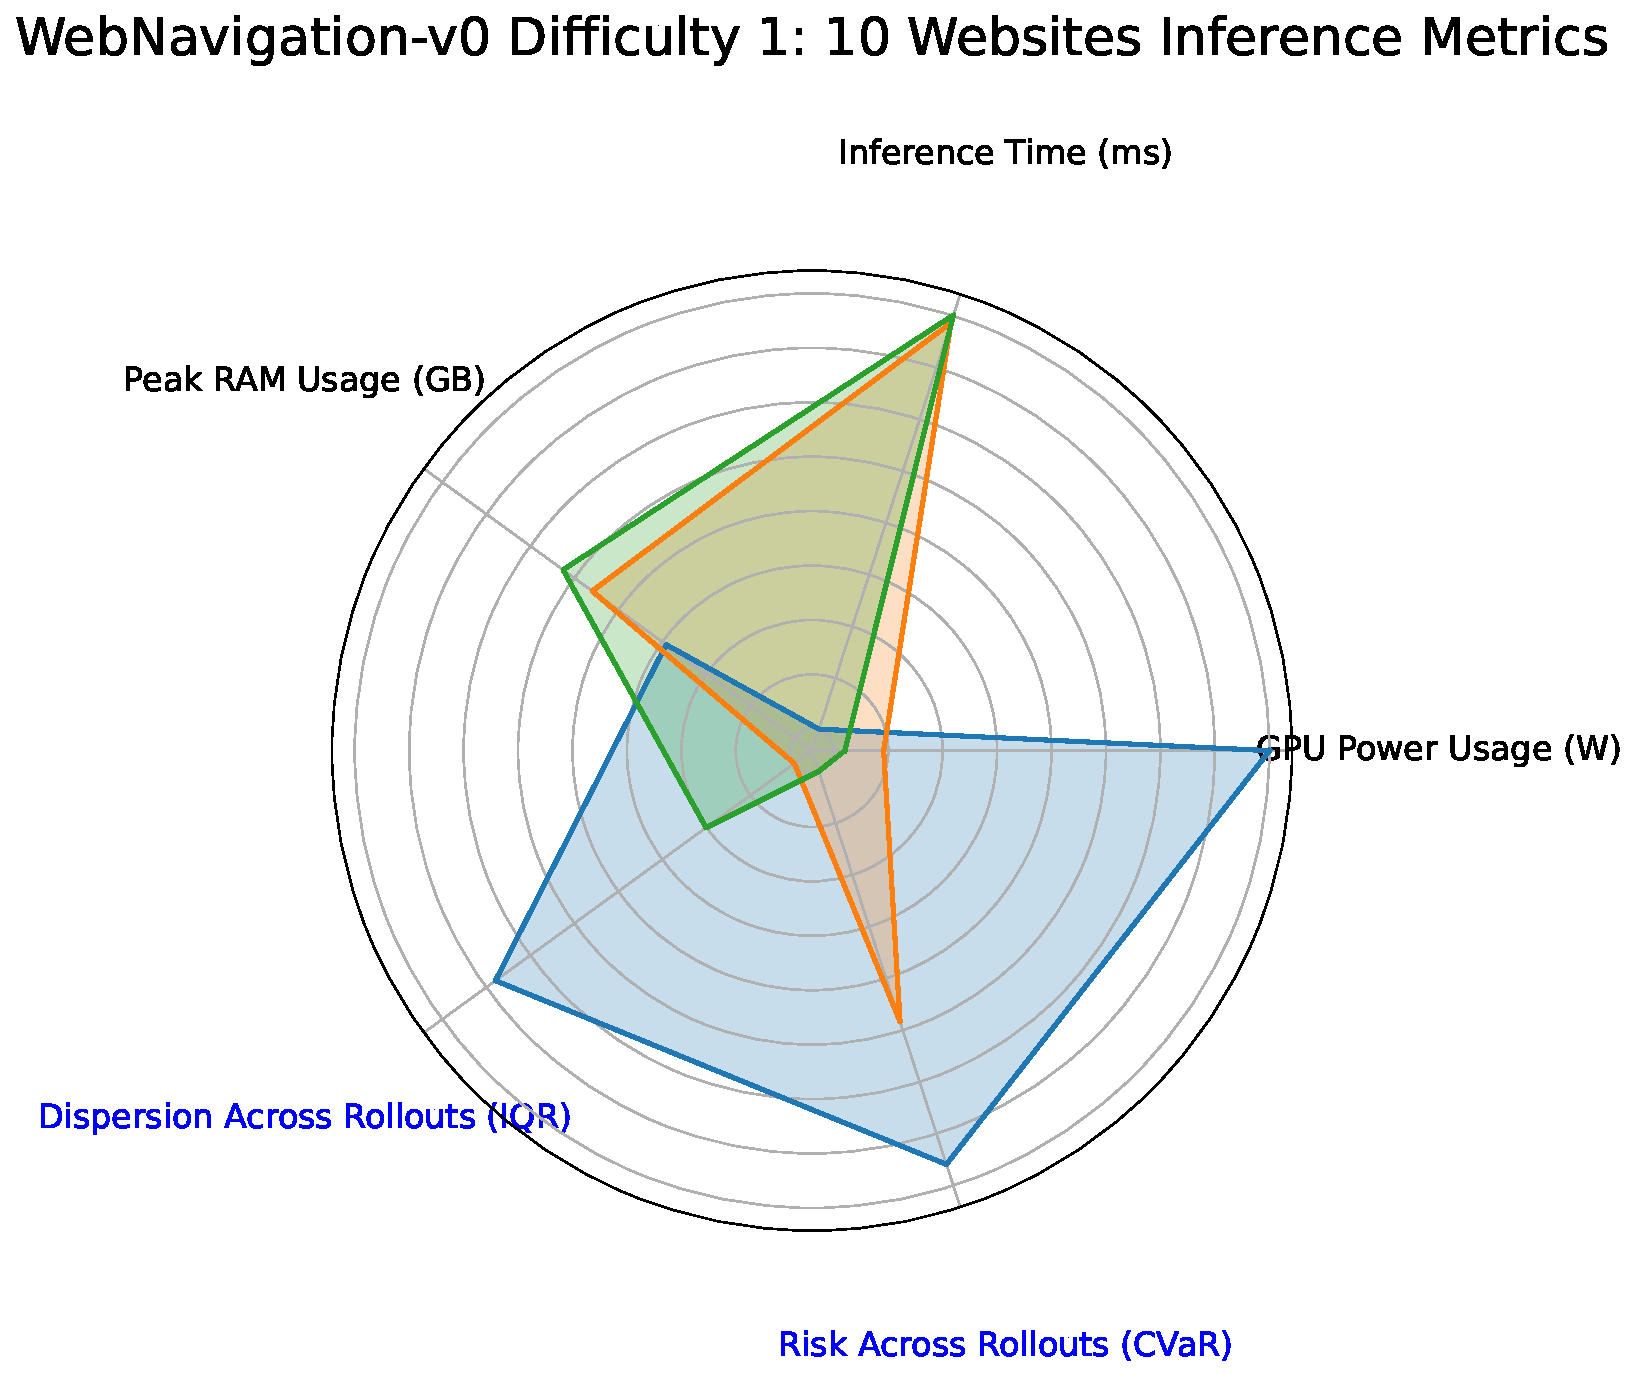
\includegraphics[width=\linewidth]{img/web_nav/WebNavigation-v0 Difficulty 1_ 10 Websites Inference Metrics.pdf}
  \end{minipage}
  \caption{Graphical representation of metrics for the "difficulty 1, 10 websites" task of WebNavigation-v0}
  \label{fig:appendix_radar_web_nav_difficulty1_10websites}
\end{figure}



\section{Experimental Setup}
\label{appendix:experimental_setup}
% \subsection{Training}
% We used the Tensorflow Agents \cite{TFAgents} library to conduct distributed reinforcement learning experiments across the three domains: computer chip floorplanning, web navigation, and quadruped locomotion.
% Our training setup consisted of one training server equipped with four A100 GPUs and multiple collect servers running in parallel.
% The number of collect jobs running simultaneously varied depending on the specific domain and the available resources (such as CPU and memory) on the collect machines, which are important for running the environments efficiently.
% When using a collect machine with 96 vCPUs, we adjusted the number of environment instances based on the computational requirements of each domain:

% \begin{enumerate}

% \item \textbf{Quadruped Locomotion}: With 96 vCPUs on the collect machine, we ran 44 quadruped locomotion environment instances concurrently.
% \item \textbf{Computer Chip Floorplanning}: For the computer chip floorplanning domain, we ran 25 computer chip floorplanning environment instances on a collect machine with 96 vCPUs.

% \item \textbf{Web Navigation}: When running web navigation experiments on a collect machine with 96 vCPUs, we instantiated 40 web navigation environment instances simultaneously.

% \end{enumerate}
% The behavioral cloning experiments for all three domains used the same setup as the online training experiments, with one training server equipped with four A100 GPUs.

% \subsection{Inference}
% For the inference phase, we used a single machine equipped with one V100 GPU to evaluate the trained models across all three domains: computer chip floorplanning, web navigation, and quadruped locomotion.
% The difference in hardware between the training and inference setups does not affect the application performance metrics, as these metrics are independent of the hardware and reflect the effectiveness of the trained models. However, the system performance metrics, such as inference time and memory usage, may vary depending on the specific hardware used during inference.

\subsection{Training}
We used the Tensorflow Agents \cite{TFAgents} library to conduct distributed reinforcement learning experiments across the three domains: computer chip floorplanning, web navigation, and quadruped locomotion.
Our training setup consisted of one training server (a Google Cloud a2-highgpu-8g instance\protect\footnotemark[1]) equipped with four NVIDIA A100 GPUs, and multiple collect servers (Google Cloud n2-standard-96 instances\protect\footnotemark[2]) with 96 vCPUs running in parallel.

\footnotetext[1]{\href{https://cloud.google.com/compute/docs/gpus\#a100-gpus}{cloud.google.com/compute/docs/gpus}}
\footnotetext[2]{\href{https://cloud.google.com/compute/docs/general-purpose-machines\#n2-standard}{cloud.google.com/compute/docs/general-purpose-machines}}

The number of collect jobs running simultaneously varied depending on the specific domain and the available resources (such as CPU and memory) on the collect machines, which are important for running the environments efficiently. When using a collect machine with 96 vCPUs, we adjusted the number of environment instances based on the computational requirements of each domain:

\begin{enumerate}
\item \textbf{Quadruped Locomotion}: With 96 vCPUs on the collect machine, we ran 44 quadruped locomotion environment instances concurrently using Python 3.9.
\item \textbf{Computer Chip Floorplanning}: For the computer chip floorplanning domain, we ran 25 computer chip floorplanning environment instances on a collect machine with 96 vCPUs using Python 3.10.
\item \textbf{Web Navigation}: When running web navigation experiments on a collect machine with 96 vCPUs, we instantiated 40 web navigation environment instances simultaneously using Python 3.10.
\end{enumerate}

The behavioral cloning experiments for all three domains used the same setup as the online training experiments, with one training server equipped with four A100 GPUs.

\subsection{Inference}
For the inference phase, we used a single machine equipped with one NVIDIA V100 GPU to evaluate the trained models across all three domains: computer chip floorplanning, web navigation, and quadruped locomotion. The difference in hardware between the training and inference setups does not affect the application performance metrics, as these metrics are independent of the hardware and reflect the effectiveness of the trained models. However, the system performance metrics, such as inference time and memory usage, may vary depending on the specific hardware used during inference.

\section{Hyperparameters}
\label{appendix:hyperparameters}
\begin{table}[H]
\centering
\begin{tabular}{|l|l|l|l|}
\hline
\textbf{Hyperparameter} & \textbf{BC} & \textbf{PPO} & \textbf{DDQN} \\ \hline
\multicolumn{4}{|c|}{\textbf{Toy Macro Standard Cell}} \\ \hline
Batch Size & 64 & 128 & 256 \\ \hline
Learning Rate & 1e-4 & 4e-4 & 4e-5 \\ \hline
Environment Batch Size & - & 512 & 512 \\ \hline
Number of Epochs & - & 6 & - \\ \hline
Number of Iterations & 200 & 5000 & 10000 \\ \hline
Entropy Regularization & - & 1e-2 & - \\ \hline
Number of Episodes Per Iteration & - & 32 & - \\ \hline
Epsilon Greedy & - & - & 0.3 \\ \hline
Replay Buffer Capacity & - & - & 1000000 \\ \hline
\multicolumn{4}{|c|}{\textbf{Ariane}} \\ \hline
Batch Size & 64 & 128 & 256 \\ \hline
Learning Rate & 1e-4 & 4e-4 & 4e-5 \\ \hline
Environment Batch Size & - & 512 & 512 \\ \hline
Number of Epochs & - & 4 & - \\ \hline
Number of Iterations & 200 & 250 & 100000 \\ \hline
Entropy Regularization & - & 1e-2 & - \\ \hline
Number of Episodes Per Iteration & - & 1024 & - \\ \hline
Epsilon Greedy & - & - & 0.3 \\ \hline
Replay Buffer Capacity & - & - & 10000000 \\ \hline
\end{tabular}
\vspace{0.5em}
\caption{Circuit Training Hyperparameters}

\end{table}


\begin{table}[H]
\centering
\begin{tabular}{|l|l|l|l|}
\hline
\textbf{Hyperparameter} & \textbf{BC} & \textbf{PPO} & \textbf{DDQN} \\ \hline
Batch Size & 128 & 128 & 128 \\ \hline
Learning Rate & 1e-4 & 3e-6 & 3e-6 \\ \hline
Entropy Regularization & - & 1e-2 & - \\ \hline
Number of Episodes Per Iteration & - & 512 & - \\ \hline
Environment Batch Size & - & 512 & 512 \\ \hline
Number of Epochs & - & 4 & - \\ \hline
Number of Iterations & 5000 & 200 & 50000 \\ \hline
Epsilon Greedy & - & - & 0.3 \\ \hline
Replay Buffer Capacity & - & - & 1000000 \\ \hline
Maximum Vocabulary Size & 500 & 500 & 500 \\ \hline
Latent Dimension & 50 & 50 & 50 \\ \hline
Embedding Dimension & 100 & 100 & 100 \\ \hline
Profile Value Dropout & 1.0 & 1.0 & 1.0 \\ \hline
\end{tabular}
\vspace{0.5em}
\caption{Web Navigation Hyperparameters}
\end{table}

\begin{table}[H]
\centering
\begin{tabular}{|l|l|l|l|}
\hline
\textbf{Hyperparameter} & \textbf{BC} & \textbf{PPO} & \textbf{SAC} \\ \hline
Batch Size & 64 & 128 & 256 \\ \hline
Learning Rate & 1e-4 & 1e-5 & 3e-4 \\ \hline
Environment Batch Size & - & 512 & 512 \\ \hline
Number of Epochs & - & 4 & - \\ \hline
Number of Iterations & 1000 & 8000 & 2000000 \\ \hline
Entropy Regularization & - & 1e-2 & - \\ \hline
Number of Episodes Per Iteration & - & 512 & - \\ \hline
Replay Buffer Capacity & - & - & 2000000 \\ \hline
\end{tabular}
\vspace{0.5em}
\caption{Quadruped Locomotion Hyperparameters}

\end{table}




\section{Dataset Collection}
\label{appendix:dataset_collection}
To collect datasets for each domain and task, we periodically saved the policies at fixed intervals throughout the training process. We then evaluated all the saved policies on 100 episodes for each domain and task.
Based on these evaluations, we created a distribution of median returns and assigned an \texttt{expertise} level to each policy as follows:
\begin{enumerate}
\item \texttt{Novice}: The median return lies within one standard deviation below the mean.
\item \texttt{Intermediate}: The median return is within one standard deviation above or below the mean.
\item \texttt{Expert}: The median return is one standard deviation above the mean or higher.
\end{enumerate}
In some cases, certain domains or tasks were too challenging, resulting in no policies of a given skill level. In such instances, we only provide a \texttt{novice} dataset.


\section{Dataset Information}
\label{appendix:dataset_information}
\begin{enumerate}
\item Dataset documentation and intended uses:
\begin{itemize}
\item The A2Perf datasets consist of data collected from three simulated environments: computer chip floorplanning, web navigation, and quadruped locomotion. The data was generated by running reinforcement learning policies at various stages of training, capturing the experiences of these policies interacting with the respective environments. The datasets are intended for use in offline reinforcement learning, imitation learning, and hybrid approaches, allowing researchers to evaluate and compare different algorithms without the need for online data collection.
\end{itemize}
\item Dataset availability:

\begin{itemize}
\item The datasets can be accessed at:
\begin{itemize}
\item Circuit Training: \url{https://drive.google.com/drive/folders/1UMhLlnYmfbnjBPN_JwVy4YXDUahXrWf6}
\item Quadruped Locomotion: \url{https://drive.google.com/drive/folders/1n1BJFip-reSPif8Bv3jXAnSOgfQAEje7}
\item Web Navigation: \url{https://drive.google.com/drive/folders/13EmCscVatl7Q5EFdWFRpwKlA2yRfonE5}
\end{itemize}
\end{itemize}

\item Data format and usage:
\begin{itemize}
\item The datasets are provided in the widely-used HDF5 format, a data model and file format designed for efficient storage and retrieval of large datasets. Detailed instructions on how to read and use the data with the Minari framework are provided at: \url{https://minari.farama.org/}
\end{itemize}
\item Licensing:
\begin{itemize}
\item The A2Perf datasets are released under the MIT License. The authors confirm that they bear all responsibility in case of violation of rights.
\end{itemize}
\item Maintenance and long-term preservation:
\begin{itemize}
\item The datasets are hosted on a Google Cloud Bucket maintained by the Farama Foundation, a non-profit organization dedicated to supporting open-source machine learning projects. This ensures the long-term availability and accessibility of the datasets for the research community.
\end{itemize}
\end{enumerate}


\section{Software Usage}
\label{appendix:software_usage}
A2Perf is a benchmark harness designed to be used flexibly on various machines. The user has the option to either run it in a Docker container or to run the benchmark locally. A Docker container is available in the harness and can be adapted to your needs. If you would like to run the benchmark locally, a guide is available to install the A2Perf benchmark harness on your Linux or MacOS system. While you can benchmark on both operating systems, it is important to note that system performance metrics are tracked using CodeCarbon. This allows to capture energy, power and memory usage at regular time intervals, and uses pyRAPL to compute the Running Average Power Limit (RAPL). However, RAPL uniquely measures power consumption information for Intel CPUs, DRAM for server architectures and GPU for client architectures. When using systems using CPU architectures different then the Intel CPUs, the power consumption metric will return a computed estimate rather than a measured metric.

The benchmark harness allows you to benchmark both the training and inference of your algorithm and agents respectively. In order to benchmark your algorithms, you need to create a submission folder which includes several files which A2Perf calls. First, a training file, \texttt{train.py} contains a function \texttt{train()}, which starts the training process of your algorithm when called. Similarly, \texttt{inference.py} covers the inference of your trained model. This file includes several functions responsible for the loading of your trained model, preprocessing observations and running inference on your model. Using a \texttt{requirements.txt} file, additional Python packages and versioning can be specified. Running the benchmark is done through a command line interface. Using flags, we can pass additional information to the submission to set up the benchmark. A \texttt{gin\_config} flag allows the user to define the settings for your environment and training process. Additionally, we need to pass the path to the submission folder using the \texttt{participant\_module\_path} flag. For a more detailed description, tutorials are available in the repository.



\section{Website Generation \& Agent Interaction}
\label{appendix:website_generation}
To create environments for the web navigation tasks, we generate synthetic websites that agents must learn to navigate. These websites serve as training and evaluation environments, where agents need to fill forms and interact with various web elements. Here we describe our procedural website generation process.

To generate the set of websites $W$, we first assume a target number of websites, denoted as $N_{\text{websites}}$.
Following the approach in \citet{gur2021environment} (shown in Table 4 of the paper), we consider 42 possible primitives that can be added to a web page and introduce two additional primitives: a "new page" primitive and a "stop" primitive, resulting in a total of 44 primitives.

The website generation process begins with an empty web page.
We repeatedly sample uniformly from the 44 primitives and add them to the current page.
If the "new page" primitive is selected during the sampling process, we start adding primitives to a new linked page.
If the "stop" primitive is selected, we conclude the generation of the current website and proceed to generate the next website, if necessary.
This process continues until we have generated the desired number of websites, $N_{\text{websites}}$.
Each website in the resulting set $W$ consists of one or more web pages, with each page containing a sampled set of primitives.

We define the difficulty of a web page as the probability of a random agent interacting with the correct primitive(s).
The difficulty of page $p_i$ is given by $-\log \left (\frac{n_{\text{active}}}{n_\text{active}+n_\text{passive}} \right )$, where $n_{\text{active}}$ and $n_{\text{passive}}$ denote the number of active and passive primitives on the page, respectively.
The difficulty of an entire sequence of web pages is determined by summing the difficulty of all individual pages it contains.
Based on these difficulty calculations, we partition the websites into three difficulty levels.
The three levels of difficulty correspond to the probability thresholds of 50\%, 25\%, and 10\% for levels 1, 2, and 3, respectively.
Users can select a specific difficulty level of web navigation by executing Python commands such as \verb|env = gym.make("WebNavigation-Difficulty-01-v0", num_websites=1)|, where the \verb|num_websites| argument defines the pool of websites available for the environment. During training or evaluation, each episode begins by randomly selecting one website from this pool at the specified difficulty level. For example, if \verb|num_websites=10|, the environment will generate 10 websites at the specified difficulty level, and each episode will randomly assign one of these websites for the agent to navigate.
At each timestep, the agent can interact with an HTML element on the page, such as modifying the text field or clicking on the element, with the objective of entering correct information into forms and clicking "next" or "submit" to advance between web pages.

% To generate the initial set $P$ of web pages, we first determined the number of pages $N_{\text{pages}}$, such that $|P| = N_{\text{pages}}$, and set the maximum number of primitives per page as $N_{\text{prim}}$. Following the approach in~\cite{gur2021environment} (Table 4), we selected 42 possible primitives to be added to a blank web page. Next, we uniformly sampled a random number of primitives between 0 and $N_{\text{prim}}$, and added these selected primitives to the page. This process resulted in a collection of single web pages, each with a distinct configuration of primitives.
% After generating the pages, we proceeded to create a set of websites, denoted by $W$. Initially, we set $W$ equal to $P$. We then generated additional web pages by randomly selecting two websites, $w_i$ and $w_j$, from $W$, and linking the final page of $w_i$ to the first page of $w_j$. Since gMiniWob currently only supports single connections between pages, passive primitives on a page terminate the interaction, while active primitives allow the agent to continue filling out the web form.
% For pages without sampled active primitives, an active primitive (submit button) is added to ensure that the agent can proceed.

% After generating a fixed number of websites, we partitioned these websites into three difficulty levels. For instance, users can select a specific difficulty level of web navigation by executing Python commands such as \texttt{env = gym.make('WebNavigation-v0', difficulty=1, num\_websites=1)}, where the \texttt{num\_websites} argument defines the number of websites that are generated for this environment.
% Ranking the websites by difficulty was done by analysing the performance of random agents. The three levels of difficulty are defined by a random agent successfully completing a website with a probability higher than \% 50, \% 25 and \%10 percent for levels 1, 2 and 3 respectively.
% To address this, we defined the difficulty of a web page as the probability of interacting with the correct primitive(s).
% The difficulty of page $p_i$ is then given by $- \log \left (\frac{n_{\text{active}}}{n_\text{active}+n_\text{passive}} \right )$, where $n_{\text{active}}$ and $n_{\text{passive}}$ denote the number of active and passive primitives on the page, respectively.
% The difficulty of an entire sequence of web pages is determined by summing the difficulty of all individual pages it contains.

% At each timestep, the agent can interact with an HTML element on the page, such as modifying the text field or clicking on the element, with the objective of entering correct information into forms and clicking "next" or "submit" to advance between webpages.

% \begin{figure}[H]
%     \centering
%     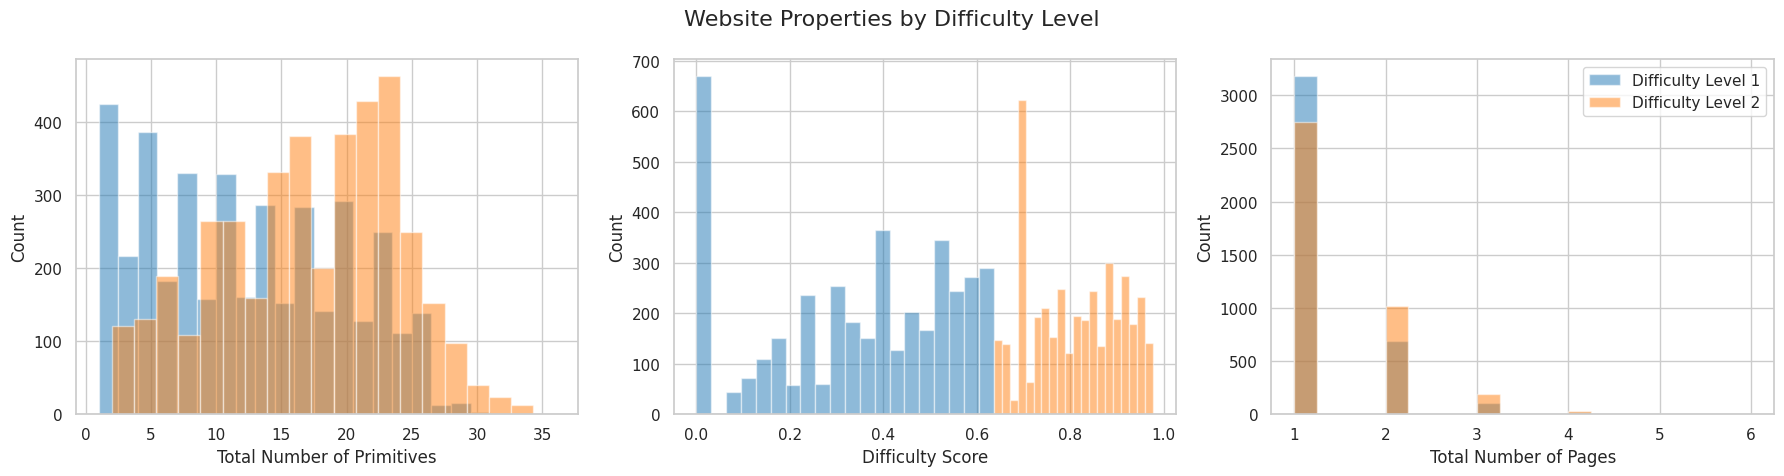
\includegraphics[width=\linewidth]{img/web_nav/website_properties_difficulty_levels_1_2.png}
%     % \caption{Caption}
%     \label{fig:enter-label1}
% \end{figure}
% \vspace{-1.10cm}
% \begin{figure}[H]
%     \centering
%     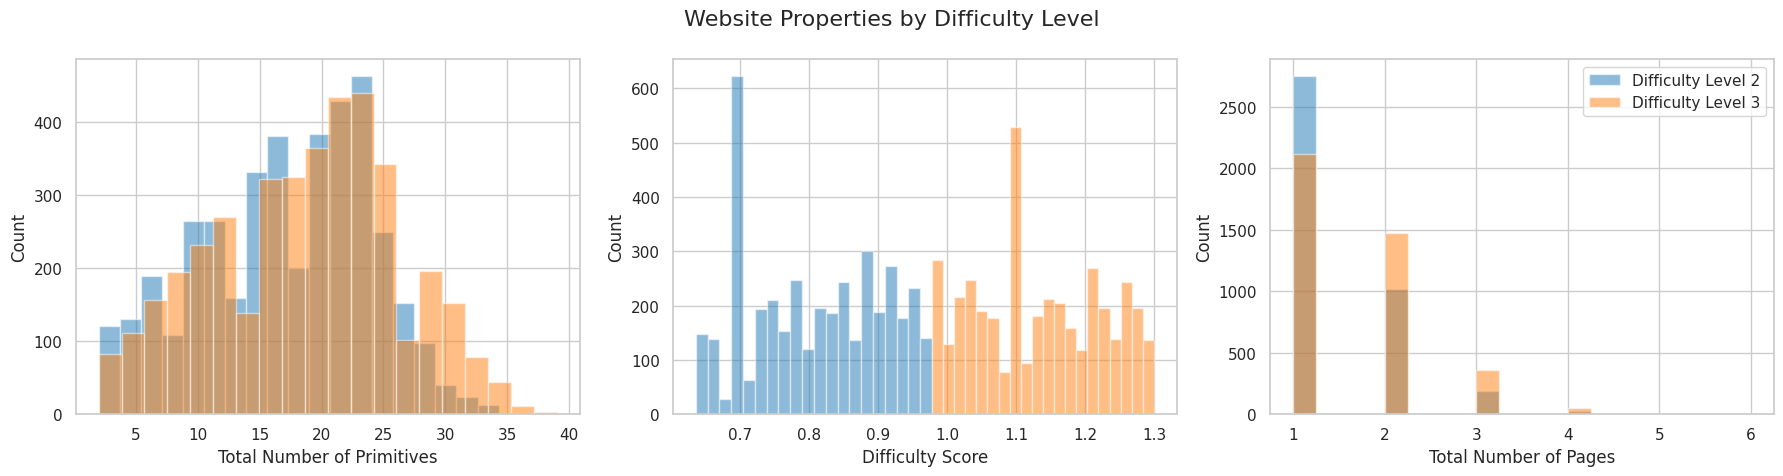
\includegraphics[width=\linewidth]{img/web_nav/website_properties_difficulty_levels_2_3.png}
%     % \caption{Caption}
%     \label{fig:enter-label2}
% \end{figure}
% \vspace{-1.10cm}

% \begin{figure}[H]
%     \centering
%     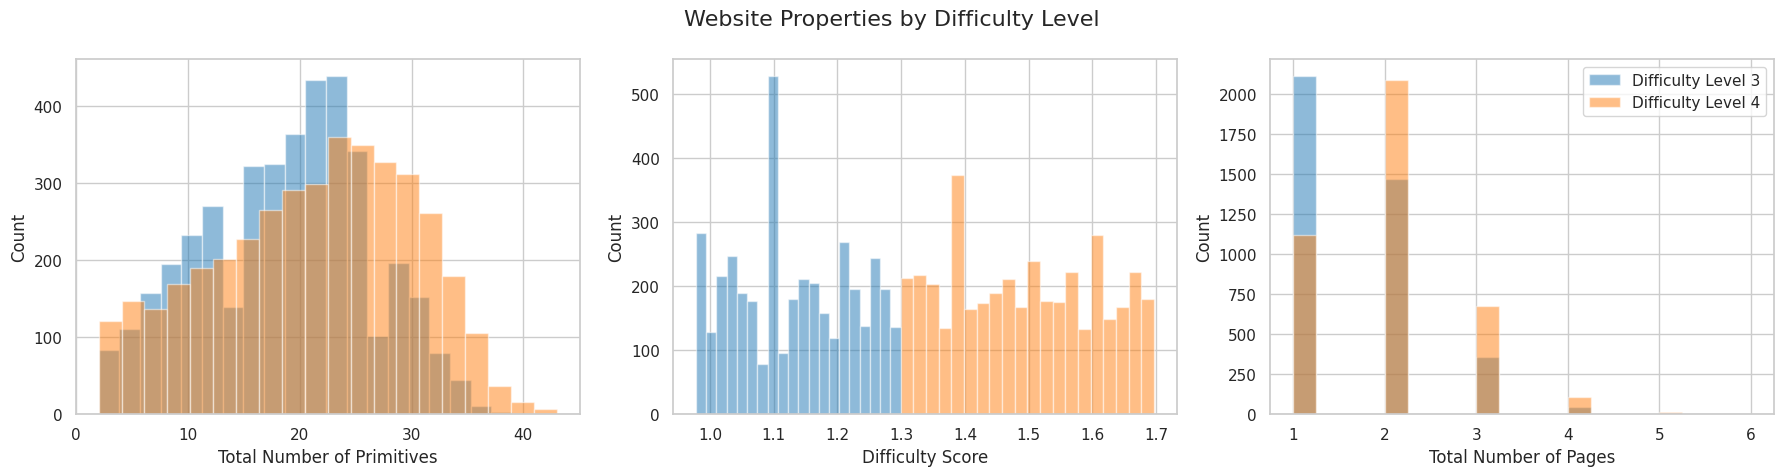
\includegraphics[width=\linewidth]{img/web_nav/website_properties_difficulty_levels_3_4.png}
%     % \caption{Caption}
%     \label{fig:enter-label3}
% \end{figure}
% \vspace{-1.10cm}

% \begin{figure}[H]
%     \centering
%     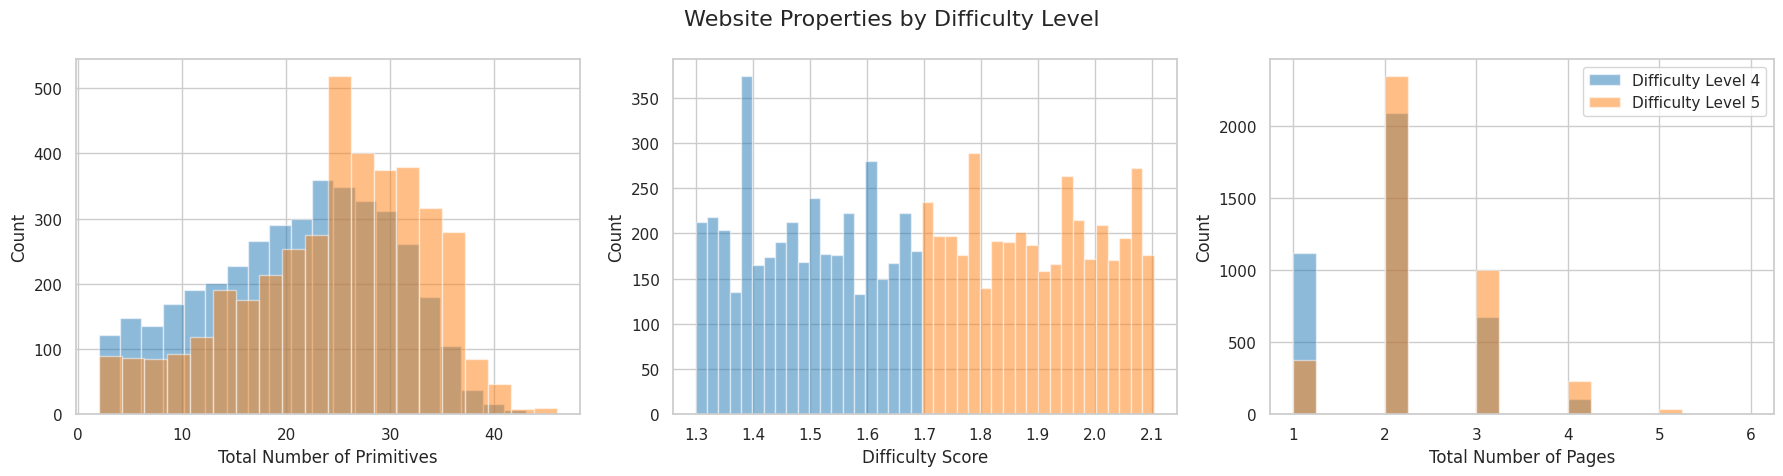
\includegraphics[width=\linewidth]{img/web_nav/website_properties_difficulty_levels_4_5.png}
%     % \caption{Caption}
%     \label{fig:enter-label4}
% \end{figure}
% \vspace{-1.10cm}

% \begin{figure}[H]
%     \centering
%     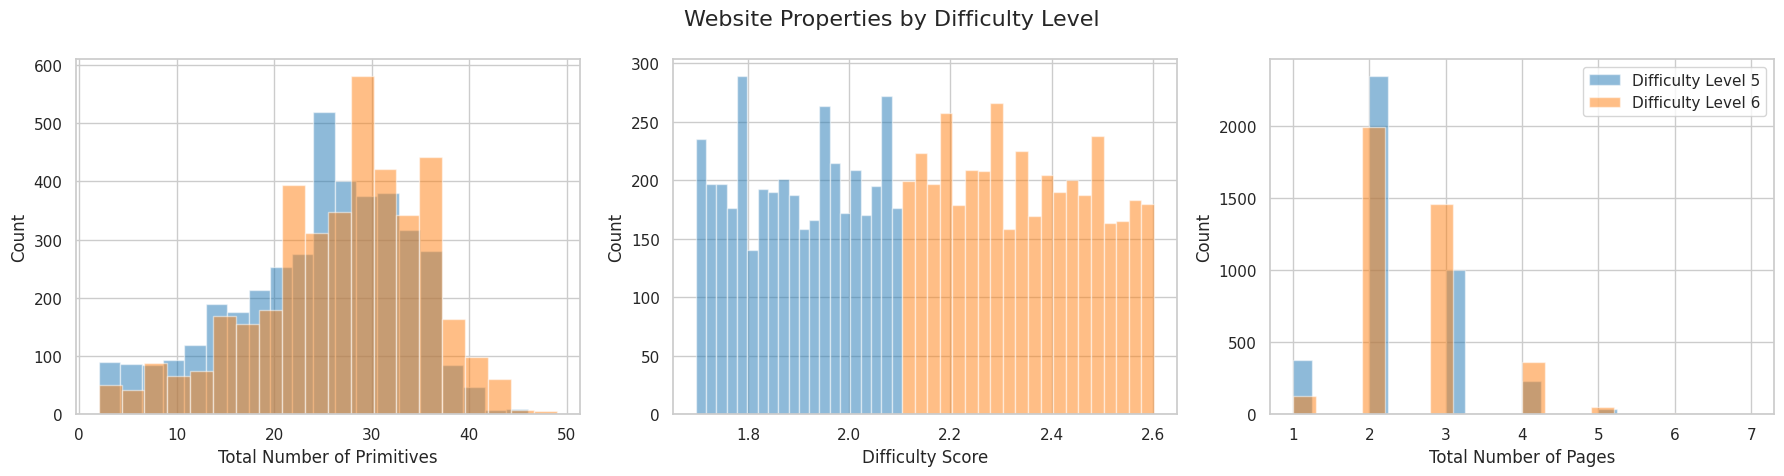
\includegraphics[width=\linewidth]{img/web_nav/website_properties_difficulty_levels_5_6.png}
%     % \caption{Caption}
%     \label{fig:enter-label5}
% \end{figure}
% \vspace{-1.10cm}

% \begin{figure}[H]
%     \centering
%     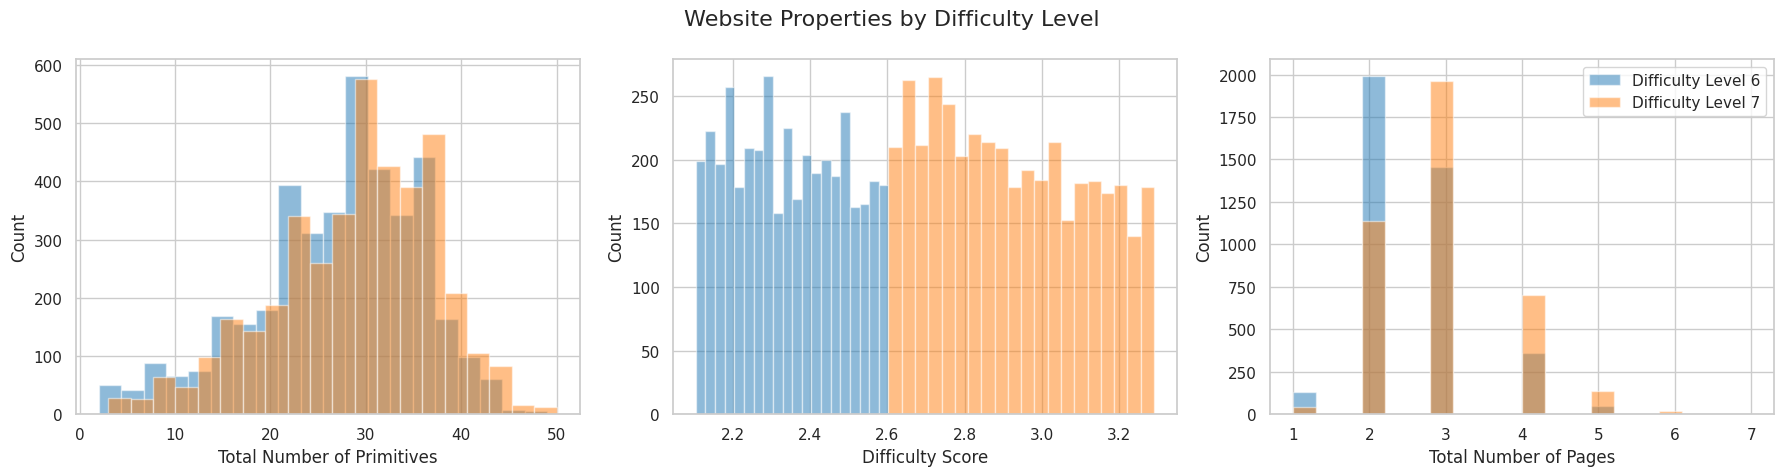
\includegraphics[width=\linewidth]{img/web_nav/website_properties_difficulty_levels_6_7.png}
%     % \caption{Caption}
%     \label{fig:enter-label6}
% \end{figure}
% \vspace{-1.10cm}

% \begin{figure}[H]
%     \centering
%     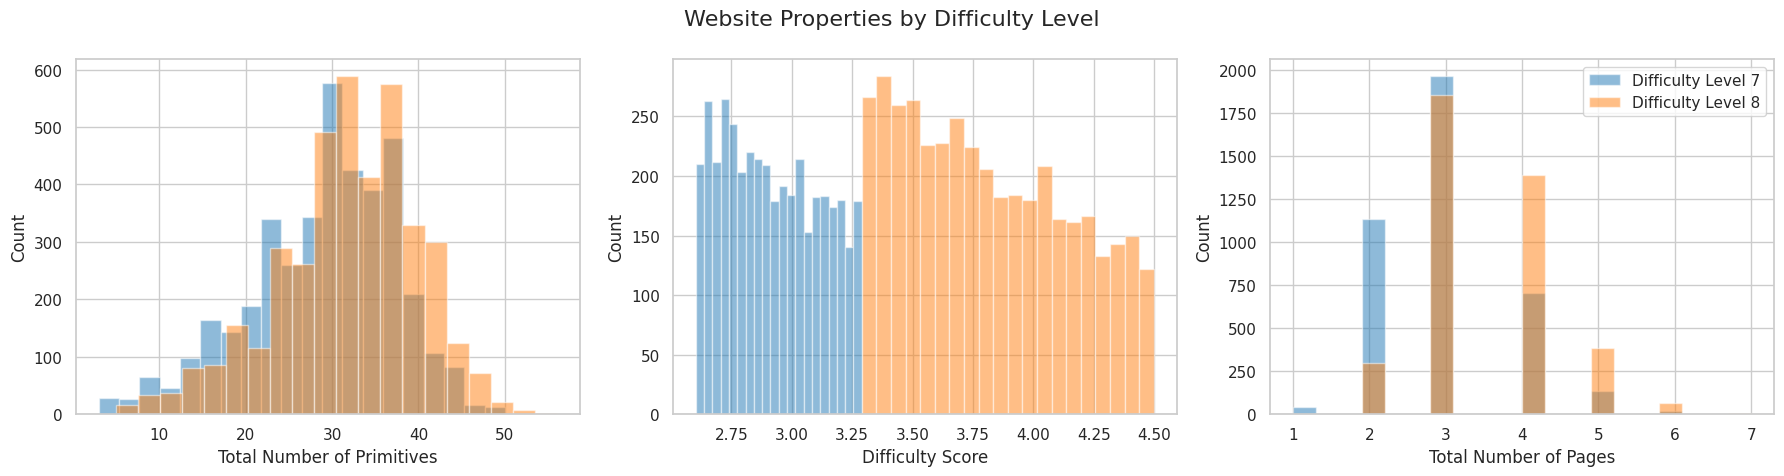
\includegraphics[width=\linewidth]{img/web_nav/website_properties_difficulty_levels_7_8.png}
%     % \caption{Caption}
%     \label{fig:enter-label7}
% \end{figure}
% \vspace{-1.10cm}

% \begin{figure}[H]
%     \centering
%     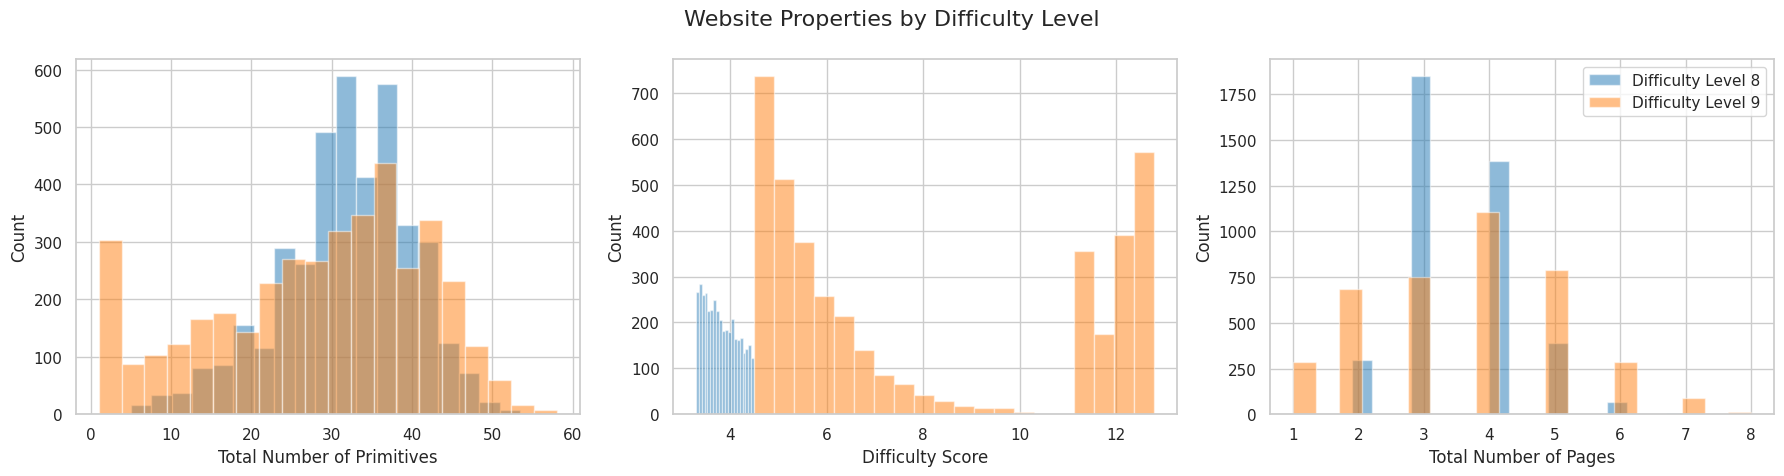
\includegraphics[width=\linewidth]{img/web_nav/website_properties_difficulty_levels_8_9.png}
%     % \caption{Caption}
%     \label{fig:enter-label8}
% \end{figure}


